\documentclass[12pt,a4paper]{article}

% --- Typography & Encodings ---
\usepackage[utf8]{inputenc}
\usepackage[english]{babel}
\usepackage{times}
\renewcommand{\ttdefault}{\rmdefault} 
\usepackage{geometry}
\geometry{
    a4paper,
    top=2.5cm,
    bottom=2.5cm,
    left=3.0cm,
    right=2.0cm
}
\usepackage{setspace}
\setstretch{1.25}

% --- Visuals, Figures & Tables ---
\usepackage{graphicx}
\usepackage{float}
\usepackage{booktabs}
\usepackage{tabularx}
\usepackage{xltabular}
\usepackage{amsmath}
\usepackage{amssymb}
\usepackage{enumitem}
\usepackage{hyperref}
\hypersetup{
    colorlinks=true,
    linkcolor=blue,
    urlcolor=blue,
    citecolor=blue
}

\begin{document}

\begin{titlepage}
\centering

{\large \textbf{HO CHI MINH CITY UNIVERSITY OF TRANSPORT}}\\[0.2cm]
{\small FACULTY OF INFORMATION TECHNOLOGY}\\[1.0cm]

\includegraphics[width=15cm]{logo_uth.png}\\[1.2cm]
\vspace{1.2cm}

{\Large \textbf{CAPSTONE PROJECT REPORT}}\\[0.4cm]
{\small COURSE: SOFTWARE ENGINEERING}\\[0.6cm]
{\LARGE \textbf{PERSONALIZED ADAPTIVE LEARNING PLATFORM WITH INTEGRATED AI TUTOR}}\\[2.2cm]

\begin{minipage}[t]{0.48\textwidth}
\textbf{Project Members:}\\
Tran Duc Hai --- 036207010989 (Leader)\\
Nguyen Anh Huy --- 066207008839\\
Luu Minh Hieu --- 079201009126\\
Nguyen Huu Tri --- 079207046324\\
Nguyen Van Minh --- 064205001508
\end{minipage}
\hfill
\begin{minipage}[t]{0.48\textwidth}
\raggedleft
\textbf{Academic Advisor / Lecturer:}\\
M.Sc. Nguyen Van Chien
\end{minipage}

\vfill
{\large \textbf{Ho Chi Minh City, September 2026}}
\end{titlepage}
\pagenumbering{roman}
\tableofcontents
\newpage
\pagenumbering{arabic}


\section*{Definitions and Acronyms (Glossary)}
\addcontentsline{toc}{section}{Definitions and Acronyms (Glossary)}

\subsection*{1. Actor \& Access Control Terms}
\begin{table}[H]
\centering
\small
\renewcommand{\arraystretch}{1.3}
\begin{tabularx}{\textwidth}{p{2.6cm} p{4.2cm} X}
\toprule
\textbf{Term} & \textbf{Full Name} & \textbf{Description} \\
\midrule
Actor & System Actor & An entity interacting with the system to achieve a specific business goal. Main actors: Administrator, Teacher / Academic Manager, Student, Parent. \\
\addlinespace[0.3em]
Administrator & System Administrator & Responsible for overall system management, user accounts, permissions, AI service configuration, and monitoring. \\
\addlinespace[0.3em]
Teacher & Teacher / Academic Manager & Responsible for building learning materials, managing question banks, monitoring student results, and reviewing AI-generated content. \\
\addlinespace[0.3em]
Student & Student & Primary user who completes diagnostic assessments, learns via personalized roadmaps, practices adaptively, and interacts with AI Tutor. \\
\addlinespace[0.3em]
Parent & Parent & Monitors student learning progress, evaluation results, and receives notifications in read-only mode via Parent Portal. \\
\addlinespace[0.3em]
RBAC & Role-Based Access Control & Access control mechanism based on roles to ensure users access authorized data and functions only. \\
\addlinespace[0.3em]
Authorization & User Authorization & Process of checking user access rights after authentication to determine the functions permitted for use within the system. \\
\addlinespace[0.3em]
Authentication & User Authentication & Process of verifying user identity before allowing access to the system through a login account. \\
\addlinespace[0.3em]
JWT & JSON Web Token & Standardized token format used for authenticating user requests securely without re-login. \\
\bottomrule
\end{tabularx}
\end{table}

\subsection*{2. Mathematical \& AI Metrics}
\begin{table}[H]
\centering
\small
\renewcommand{\arraystretch}{1.3}
\begin{tabularx}{\textwidth}{p{2.4cm} p{4.4cm} X}
\toprule
\textbf{Term} & \textbf{Full Name} & \textbf{Description} \\
\midrule
$\theta$ (Theta) & Student Ability / Proficiency Level & Real-time ability measure of a student ($[-3, +3]$ or $[0, 1]$), representing mastery over a topic. \\
\addlinespace[0.3em]
$b$ & Question Difficulty Level & Standard difficulty level of a test question. Higher values indicate higher complexity. \\
\addlinespace[0.3em]
$\Delta\theta$ & Ability Modulation / Delta & The increase/decrease in ability index immediately following a correct or incorrect answer. \\
\addlinespace[0.3em]
$\pm\Delta b$ & Difficulty Tolerance Range & Allowed difficulty variance when an exact difficulty match $b$ is missing in the database. \\
\addlinespace[0.3em]
IRT & Item Response Theory & Mathematical model measuring the probability of a correct response given student ability ($\theta$) and question difficulty ($b$). \\
\addlinespace[0.3em]
BKT & Bayesian Knowledge Tracing & Algorithmic model tracing student understanding probability across sequential exercise attempts. \\
\addlinespace[0.3em]
ZPD & Zone of Proximal Development & Optimal difficulty range matching student current ability---neither too easy nor overly frustrating. \\
\bottomrule
\end{tabularx}
\end{table}

\subsection*{3. AI \& Technical Terms}
\begin{table}[H]
\centering
\small
\renewcommand{\arraystretch}{1.3}
\begin{tabularx}{\textwidth}{p{2.6cm} p{4.2cm} X}
\toprule
\textbf{Term} & \textbf{Full Name} & \textbf{Description} \\
\midrule
RAG & Retrieval-Augmented Generation & Combines external vector DB knowledge retrieval with LLM prompts to produce accurate, hallucination-free answers. \\
\addlinespace[0.3em]
LLM & Large Language Model & Large language model (OpenAI GPT, Gemini, Anthropic) serving as the natural language engine for AI Tutor. \\
\addlinespace[0.3em]
Vector DB & Vector Database & Specialized database (Milvus/Pinecone) storing vector embeddings for high-speed semantic similarity searches. \\
\addlinespace[0.3em]
Cosine Similarity & Cosine Similarity Search & Mathematical measure comparing semantic similarity between student prompts and context vectors in Vector DB. \\
\addlinespace[0.3em]
SSE & Server-Sent Events & One-way real-time streaming protocol from Server to Client for smooth word-by-word chatbot output. \\
\addlinespace[0.3em]
TTFT & Time To First Token & Latency from user prompt submission until the first response token is displayed ($< 1.5$s). \\
\bottomrule
\end{tabularx}
\end{table}
\newpage

\section{Project Introduction}

\subsection{Overview}
\subsubsection{Project Information}
\begin{itemize}
    \item \textbf{Project Title:} Personalized Adaptive Learning Platform with Integrated AI Tutor
    \item \textbf{Domain:} Educational Technology (EdTech), Adaptive Learning Systems, Artificial Intelligence in Education.
    \item \textbf{Primary Target:} National Competency Assessment Examination preparation and standardized academic evaluation.
\end{itemize}

\subsubsection{Project Team \& Responsibilities}
\begin{table}[H]
\centering
\small
\renewcommand{\arraystretch}{1.3}
\begin{tabularx}{\textwidth}{l l X l}
\toprule
\textbf{Full Name} & \textbf{Role} & \textbf{Email} & \textbf{Phone} \\
\midrule
Nguyen Van Chien & Lecturer & chiennv@ut.edu.vn & 0986964972 \\
Tran Duc Hai & Leader & haitd360989@ut.edu.vn & 0325932899 \\
Nguyen Anh Huy & Member & huyna668839@ut.edu.vn & 0328940225 \\
Nguyen Huu Tri & Member & trinh796324@ut.edu.vn & 0982290149 \\
Nguyen Van Minh & Member & minhnv1508@ut.edu.vn & 0342324611 \\
Luu Minh Hieu & Member & hieulm799126@ut.edu.vn & 0334466229 \\
\bottomrule
\end{tabularx}
\end{table}

\subsection{Product Background \& Problem Statement}
\subsubsection{Background}
In recent years, standardized competency exams have become a crucial benchmark for higher education admissions. However, students preparing for these exams face significant structural challenges in their study routines. Traditional test preparation relies heavily on a ``one-size-fits-all'' model, where every student follows an identical syllabus regardless of their individual baseline knowledge, strengths, or weaknesses.

\subsubsection{Problem Statement}
\begin{itemize}
    \item \textbf{Lack of Real-Time Ability Measurement:} Traditional e-learning platforms measure performance using static percentage scores rather than estimating true latent ability ($\theta$), making it difficult to pinpoint exact knowledge gaps.
    \item \textbf{Generic and Hallucination-Prone AI Assistance:} Standard conversational AI models often deliver hallucinated or unverified solutions that do not strictly adhere to verified curriculum standards.
    \item \textbf{Inflexible Learning Paths \& High Costs:} Private tutoring and offline test prep centers present high financial barriers while failing to offer dynamic, continuous adjustments based on daily student effort and cognitive overload.
\end{itemize}

\subsection{Existing Systems Comparison}
\begin{table}[H]
\centering
\small
\renewcommand{\arraystretch}{1.3}
\begin{tabularx}{\textwidth}{p{2.6cm} X X X}
\toprule
\textbf{Criteria} & \textbf{Traditional LMS \& Offline Centers} & \textbf{Generic AI Chatbot Platforms} & \textbf{Proposed Platform} \\
\midrule
Assessment Model & Fixed question sets, static scoring & Unstructured prompts & Dynamic Item Response Theory (IRT) ($\theta$ \& $b$) \\
\addlinespace[0.3em]
Learning Path & Linear, manual progression & None / Static text suggestion & Automated AI-driven Roadmap with dynamic recalibration \\
\addlinespace[0.3em]
AI Answer Accuracy & Not available & Susceptible to AI Hallucination & High accuracy via RAG Engine \& Vector DB Knowledge Base \\
\addlinespace[0.3em]
Progress Tracking & Basic score logs & None & Multi-actor Analytics (Student, Teacher, Parent) \\
\bottomrule
\end{tabularx}
\end{table}


\section{Project Management Plan}

\subsection{Overview \& Scope Estimation (WBS \& Effort Estimation)}
The project utilizes a Work Breakdown Structure (WBS) to divide total engineering effort across 4 main functional streams: Frontend/Mobile Development, Backend Infrastructure, AI/RAG Engineering, and Quality Assurance/Documentation.

\vspace{0.3cm}
\noindent\textbf{Effort Distribution (Total Estimated Effort: 600 Person-Hours / 8 Weeks)}

\begin{table}[H]
\centering
\small
\renewcommand{\arraystretch}{1.3}
\begin{tabularx}{\textwidth}{p{3.8cm} p{4.2cm} p{3.2cm} r}
\toprule
\textbf{Work Package / Task Group} & \textbf{Primary Responsibility} & \textbf{Assigned Members} & \textbf{Estimated Effort} \\
\midrule
WP1: Requirement Analysis \& System Architecture & System Architecture \& Database Design & Leader \& All Members & 80 Person-Hours \\
\addlinespace[0.3em]
WP2: AI \& Adaptive Engine Integration & IRT Algorithm, RAG Pipeline, Vector DB Setup & AI Engineers & 180 Person-Hours \\
\addlinespace[0.3em]
WP3: Core Service Backend API & RESTful APIs, JWT Auth, RBAC, Database Management & Backend Engineers & 160 Person-Hours \\
\addlinespace[0.3em]
WP4: User Interface \& Analytics & Web/Mobile Application (Student, Teacher, Parent Dashboards) & Frontend Engineers & 120 Person-Hours \\
\addlinespace[0.3em]
WP5: Testing, Deployment \& Documentation & Unit/Integration Tests, SRS/SDD Docs, Cloud Setup & QA \& Documentation Lead & 60 Person-Hours \\
\midrule
\multicolumn{3}{l}{\textbf{Total Estimated Effort (8 Weeks)}} & \textbf{600 Person-Hours} \\
\bottomrule
\end{tabularx}
\end{table}

\subsection{Project Objectives \& Quality Metrics}
To ensure the system meets academic and technical expectations, the team enforces key quantitative quality metrics across the development lifecycle:
\begin{itemize}[leftmargin=1.5em, itemsep=0.2em]
    \item \textbf{Functional Completeness:} 100\% implementation of defined Core Business Flows (UC-01 to UC-06).
    \item \textbf{Performance Benchmark:}
    \begin{itemize}[leftmargin=1.5em, itemsep=0.1em]
        \item API Response Latency $< 3.0$ seconds for standard CRUD operations.
        \item AI Tutor Time-To-First-Token (TTFT) $< 1.5$ seconds utilizing Server-Sent Events (SSE) streaming.
    \end{itemize}
    \item \textbf{AI Output Accuracy:} Hallucination rate strictly maintained $< 2.0\%$ by enforcing RAG context retrieval with Cosine Similarity thresholds ($\text{Score} \ge 0.65$).
    \item \textbf{Security \& Authorization:} 0 unauthorized data leakages across roles (RBAC) enforced with JWT authentication and Prompt Sanitization against Prompt Injection attacks.
\end{itemize}

\subsection{Project Risks \& Response Plans}
\begin{table}[H]
\centering
\small
\renewcommand{\arraystretch}{1.3}
\begin{tabularx}{\textwidth}{p{1.4cm} p{2.2cm} X p{2.0cm} X}
\toprule
\textbf{Risk ID} & \textbf{Risk Category} & \textbf{Risk Description} & \textbf{Probability / Impact} & \textbf{Mitigation \& Response Plan} \\
\midrule
RSK-01 & Technical (AI) & High LLM API latency or Service Rate Limit exceeding quota. & Medium / High & Implement Redis caching for frequent prompts; fallback to static teacher-approved solutions if LLM times out ($> 5$s). \\
\addlinespace[0.3em]
RSK-02 & Technical (Accuracy) & AI Hallucination or generating answers outside domain scope. & Medium / High & Enforce strict RAG Cosine Similarity filters; apply Guardrail rules; route low-confidence queries to Teacher Ticket queue. \\
\addlinespace[0.3em]
RSK-03 & Schedule & Scope creep or delayed API integration between Frontend and AI Backend. & High / Medium & Adopt strict Agile/Scrum weekly sprints; conduct daily standups; maintain continuous integration (CI/CD). \\
\addlinespace[0.3em]
RSK-04 & Data & Cold-start problem for Item Response Theory (IRT) difficulty calibration ($b$). & High / Medium & Pre-calibrate initial question difficulty matrices based on historical exam standards and Bloom's Taxonomy tags. \\
\bottomrule
\end{tabularx}
\end{table}

\subsection{Management Approach \& Process (Agile/Scrum 8-Week Timeline)}
The project follows an Agile/Scrum Framework over an 8-week delivery timeline, divided into 4 two-week Sprints:
\begin{itemize}[leftmargin=1.5em, itemsep=0.2em]
    \item \textbf{Week 1--2 (Sprint 1):} Requirements Analysis, SRS Documentation, Architecture \& Database Design.
    \item \textbf{Week 3--4 (Sprint 2):} Core Backend Services, IRT Engine Development, Initial Vector DB Setup.
    \item \textbf{Week 5--6 (Sprint 3):} RAG Pipeline Integration, AI Tutor Chatbot, Frontend/Mobile UI Build.
    \item \textbf{Week 7--8 (Sprint 4):} Multi-actor Analytics Dashboards, End-to-End Testing, Bug Fixing, Final Release Package.
    \item \textbf{Sprint Meetings:} Weekly Planning on Mondays; Retrospectives on Fridays.
    \item \textbf{Daily Sync:} 15-minute daily standups via Discord/Zalo to track progress and clear technical blockers.
\end{itemize}

\subsection{Project Communications \& Configuration Management}

\subsubsection{Communication Channels}
\begin{itemize}[leftmargin=1.5em, itemsep=0.2em]
    \item \textbf{Source Code Repository:} GitHub / GitLab (Main branch protection enforced; Merge Requests require at least 1 peer review).
    \item \textbf{Task \& Progress Management:} Trello / Jira board tracking Backlog, In Progress, Review, and Done.
    \item \textbf{Team Workspace:} Discord for technical discussions; Google Drive for Capstone Documentation.
\end{itemize}

\subsubsection{Configuration \& Version Control Strategy}
\begin{enumerate}[leftmargin=1.5em, itemsep=0.2em]
    \item \textbf{Git Branching Strategy:} GitFlow model (\texttt{main} for release, \texttt{develop} for integration, \texttt{feature/*} for individual task development).
    \item \textbf{API Documentation:} Postman Collection / Swagger UI for frontend-backend API integration standards.
    \item \textbf{Environment Configuration:} Separate \texttt{.env} files for Local Development, Staging, and Production (Azure Cloud) to protect sensitive credentials (JWT Secrets, AI API Keys).
\end{enumerate}


\section{Software Requirement Specification (SRS)}

\subsection{User Requirements}

\subsubsection{System Actors Analysis}

\paragraph{System Administrator}
\begin{itemize}[leftmargin=1.5em, itemsep=0.2em]
    \item \textbf{Goal:} Ensure operational stability, data security, and performance; optimize cloud and AI infrastructure costs; manage user accounts and system configuration.
    \item \textbf{Scope:} Admin Portal, Backend infrastructure, Cloud/Server environments, API Gateways, Audit Logs, and Analytics.
    \item \textbf{Permissions:} CRUD operations on all user accounts (Teacher, Student, Parent); AI/RAG engine parameter configurations; Subscription and Payment package configuration; System health and token usage monitoring.
\end{itemize}

\paragraph{Teacher / Academic Manager}
\begin{itemize}[leftmargin=1.5em, itemsep=0.2em]
    \item \textbf{Goal:} Build standardized question banks aligned with Competency Examinations; review AI-generated content (Human-in-the-loop); monitor class and student progress.
    \item \textbf{Scope:} Teacher Portal, Question Bank \& Knowledge Base (RAG Vector DB), Class Analytics Dashboard.
    \item \textbf{Permissions:} CRUD questions/exams; upload theory documents into Knowledge Base; review/edit AI-generated explanations; view class analytics and export reports.
\end{itemize}

\paragraph{Student}
\begin{itemize}[leftmargin=1.5em, itemsep=0.2em]
    \item \textbf{Goal:} Prepare efficiently for exams via personalized roadmaps; receive 24/7 AI Tutor assistance; track daily progress and achieve target scores.
    \item \textbf{Scope:} Student Web/Mobile App, AI Chatbot interface, Personal Dashboard, Learning Roadmap.
    \item \textbf{Permissions:} Update personal targets and study time; interact with AI Tutor; view competency radar charts, learning streak, and predicted scores.
\end{itemize}

\paragraph{Parent}
\begin{itemize}[leftmargin=1.5em, itemsep=0.2em]
    \item \textbf{Goal:} Monitor student learning consistency, performance, and score predictions without interfering with learning workflows.
    \item \textbf{Scope:} Parent Portal / Mobile App (Read-Only Mode).
    \item \textbf{Permissions:} Read-only access to study time, practice test scores, AI predicted scores, and automated alert notifications (absence/drop in activity).
\end{itemize}

\begin{figure}[H]
    \centering
    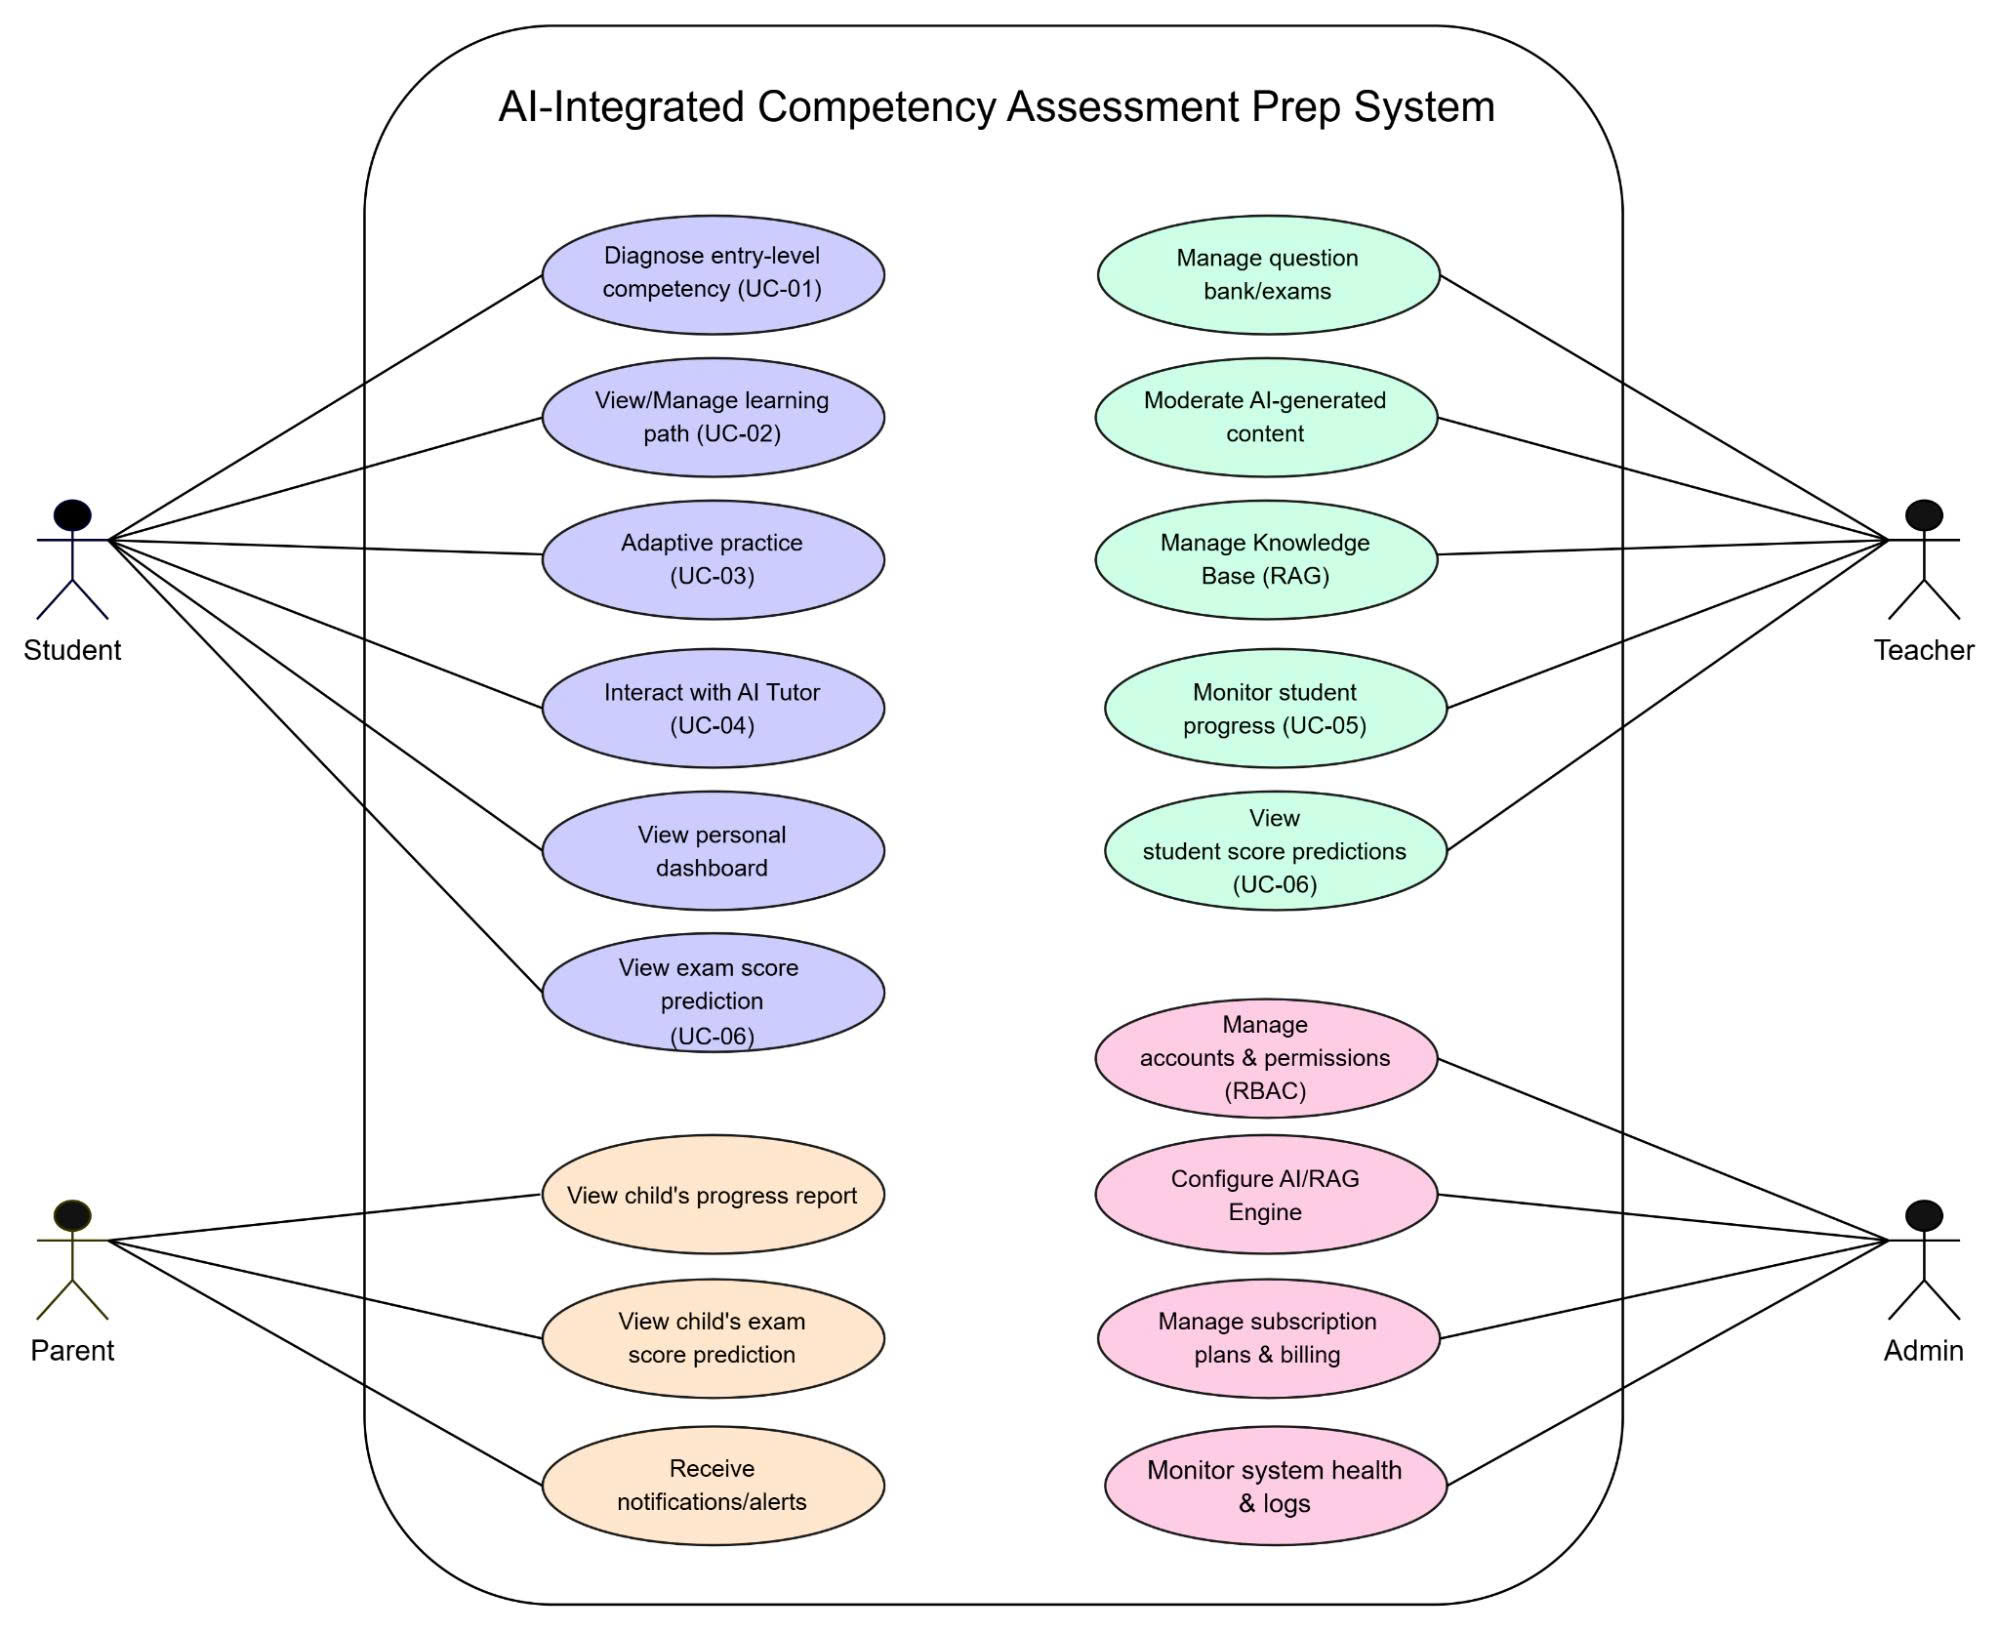
\includegraphics[width=0.88\textwidth]{figure_1_use_case.png}
    \caption{Overall System Use Case Diagram}
    \label{fig:overall_use_case}
\end{figure}

\subsection{Functional Requirements (Core Business Flows)}

\subsubsection{Core Flow 1 (UC-01): Competency Diagnosis \& Learning Profile Generation}

\noindent\textbf{Actors:} Student (Primary), Assessment Engine, AI Diagnosis Engine, Learning Database.

\vspace{0.2cm}
\noindent\textbf{Pre-conditions:} Student authenticated via JWT Token; Question Bank approved by Teacher; AI Diagnosis Engine online.

\vspace{0.2cm}
\noindent\textbf{Basic Flow:}
\begin{enumerate}[leftmargin=1.5em, itemsep=0.2em]
    \item Student initiates a Diagnostic Session via the dashboard. System validates the JWT Token and checks if an existing Learning Profile exists.
    \item Student inputs Target Score ($S_{\text{target}}$), Exam Date ($D_{\text{exam}}$), and Daily Study Time ($T_{\text{daily}}$).
    \item Assessment Engine queries Question Bank and renders standardized diagnostic test.
    \item Student completes and submits test; system logs response choices, time per question, and behavioral indicators.
    \item Assessment Engine calculates raw scores and normalizes data.
    \item AI Diagnosis Engine computes initial Proficiency Level ($\theta$), identifies Strengths, Weaknesses, Knowledge Gaps, and Learning Preferences.
    \item System constructs the Learning Profile data structure, persists it into Learning Database along with Assessment Result history, and associates it with the Student account.
    \item System renders the visual diagnostic feedback on the Student Dashboard, including Competency Levels, Knowledge Gap breakdown, Competency Radar Chart, and initial score projections.
    \item System finalizes UC-01 and forwards the generated Learning Profile data to Core Flow 2 (UC-02: AI Roadmap Generation).
\end{enumerate}

\noindent\textbf{Alternative Flows:}
\begin{itemize}[leftmargin=1.5em, itemsep=0.2em]
    \item \textbf{AF-1.1 Re-assessment:} Student triggers re-evaluation; system generates a new test variant and updates profile history.
    \item \textbf{AF-1.2 Session Interruption:} If Student disconnects or closes the browser mid-test, System persists the current session state and allows resumption upon re-login.
    \item \textbf{AF-1.3 AI Timeout:} If AI Diagnosis times out ($> 5$s), system saves raw results, sets state to ``Pending Analysis'', and notifies student.
    \item \textbf{AF-1.4 Insufficient Submission Data:} If the submitted test has excessive skipped questions and lacks minimum data for evaluation, System rejects profile generation and prompts Student to retake the test.
\end{itemize}

\noindent\textbf{Post-conditions:}
\begin{itemize}[leftmargin=1.5em, itemsep=0.2em]
    \item \textbf{Success:} Assessment result is recorded, Learning Profile is generated and persisted in the database, diagnostic feedback is displayed on Student Dashboard, and data is passed to UC-02.
    \item \textbf{Failure:} Learning Profile is not created; session state is saved or system error is logged.
\end{itemize}

\begin{figure}[H]
    \centering
    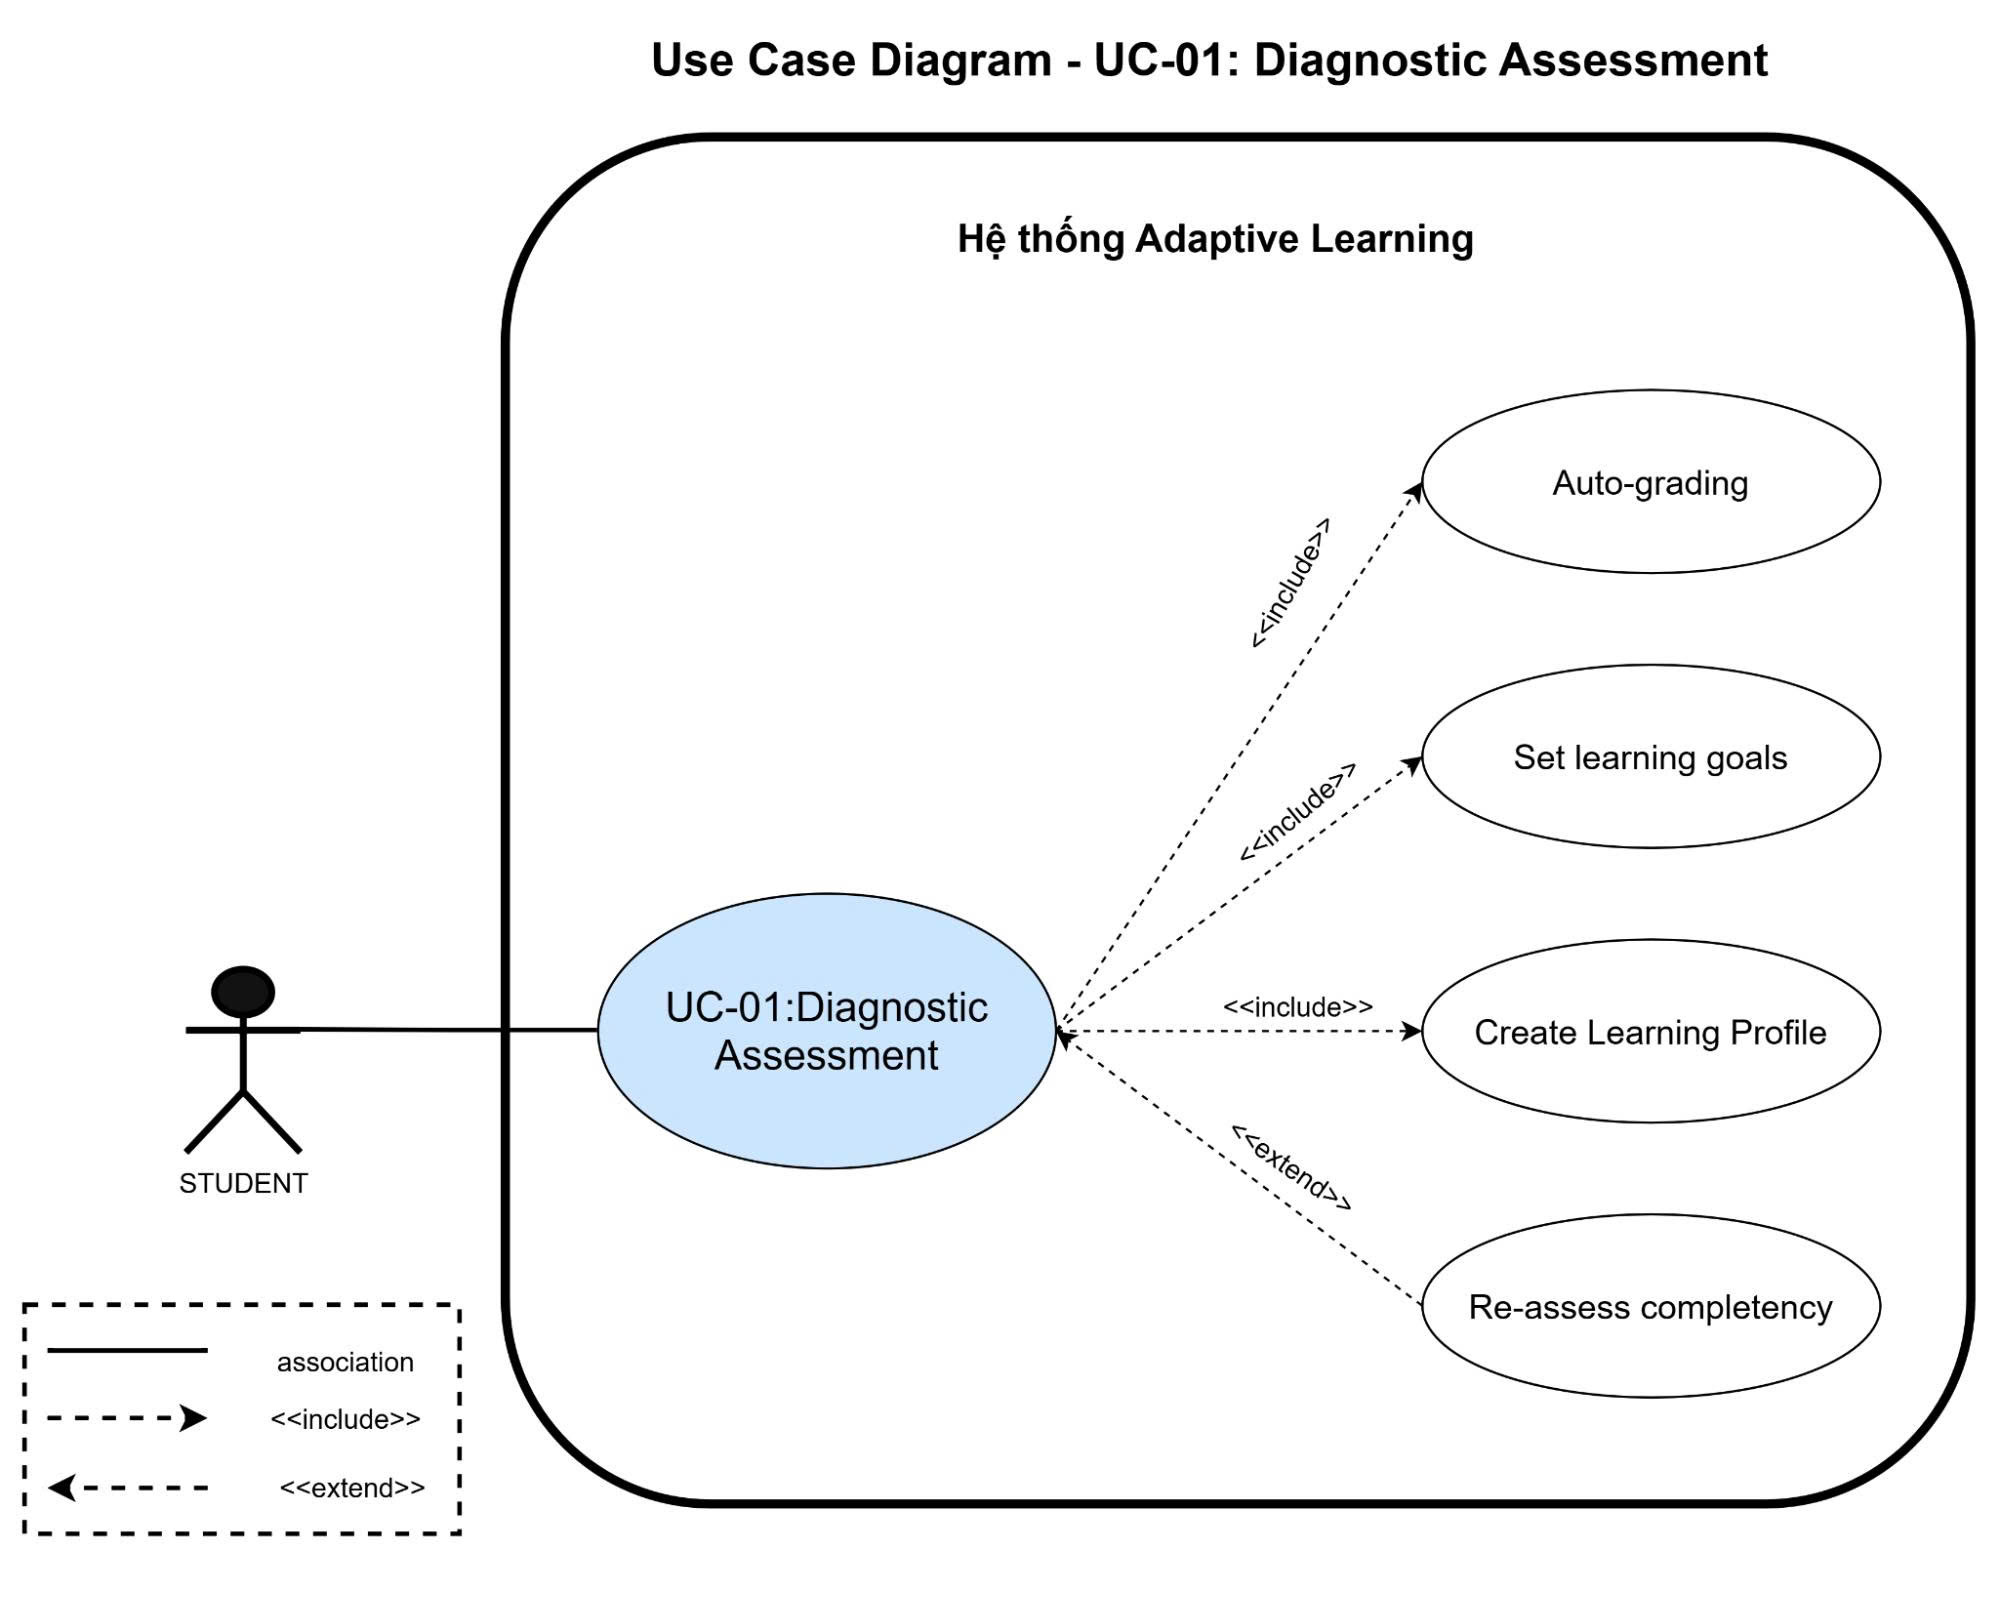
\includegraphics[width=0.75\textwidth]{figure_uc01_diagnosis.png}
    \caption{Use Case Diagram --- UC-01: Diagnostic Assessment}
    \label{fig:uc01_diag}
\end{figure}

\subsubsection{Core Flow 2 (UC-02): AI Roadmap Generation}

\noindent\textbf{Actors:} Student (Primary), AI Planner Engine, Learning Database.

\vspace{0.2cm}
\noindent\textbf{Pre-conditions:}
\begin{itemize}[leftmargin=1.5em, itemsep=0.1em]
    \item Student is authenticated and possesses a valid Learning Profile generated from UC-01.
    \item Target learning goals (Target Score $S_{\text{target}}$ from 1 to 1200, Exam Date $D_{\text{exam}}$, Daily Study Time $T_{\text{daily}}$) are defined.
    \item AI Planner Engine and Learning Database are online and operational.
\end{itemize}

\noindent\textbf{Basic Flow:}
\begin{enumerate}[leftmargin=1.5em, itemsep=0.2em]
    \item Triggered automatically after UC-01 or manually via goal updates.
    \item AI Planner retrieves latest Learning Profile and Exam Matrix.
    \item Gap Analysis is performed against $S_{\text{target}}$ and remaining days $N_{\text{days}}$.
    \item Knowledge Graph prioritizes missing prerequisite topics ($\theta < 0.5$).
    \item AI constructs phases (Foundation $\rightarrow$ Topic Mastery $\rightarrow$ Practice $\rightarrow$ Final Sprint) and generates structured JSON Daily Tasks aligned with $T_{\text{daily}}$.
    \item System saves Roadmap in DB and renders interactive timeline dashboard.
\end{enumerate}

\noindent\textbf{Alternative Flow:}
\begin{itemize}[leftmargin=1.5em, itemsep=0.2em]
    \item \textbf{AF-2.1 Unrealistic Goal:} If required effort exceeds $N_{\text{days}} \times T_{\text{daily}}$, system displays a warning and prompts student to increase daily time or lower target score.
\end{itemize}

\noindent\textbf{Post-conditions:}
\begin{itemize}[leftmargin=1.5em, itemsep=0.2em]
    \item \textbf{Success:} Personalized Study Plan and Daily Tasks are persisted in the database; interactive roadmap timeline is rendered on Student Dashboard.
    \item \textbf{Failure:} Study Plan is not generated; feasibility alert or system error message is displayed to the student.
\end{itemize}

\begin{figure}[H]
    \centering
    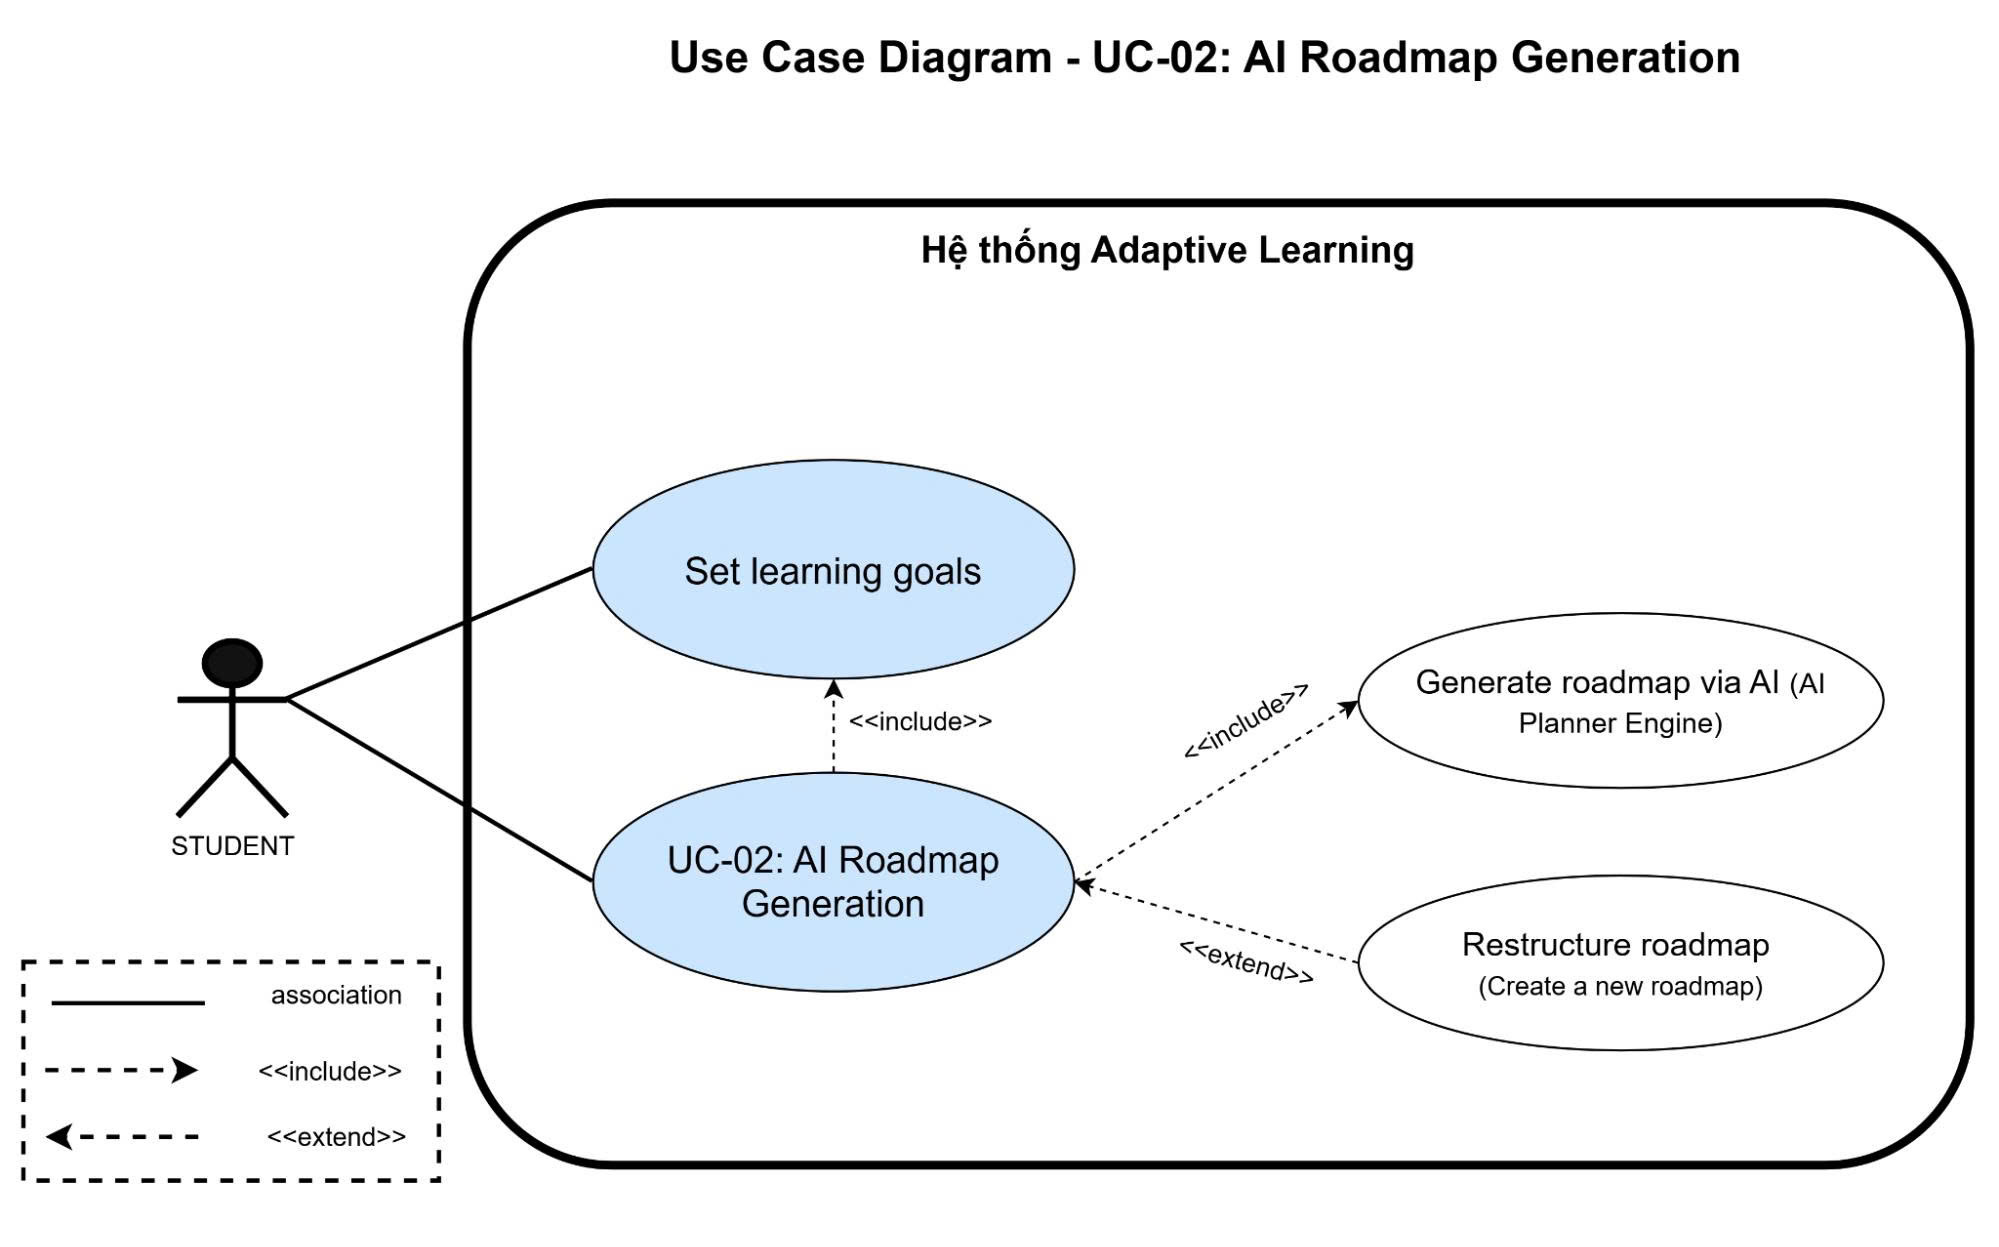
\includegraphics[width=0.9\textwidth]{figure_uc02_roadmap.png}
    \caption{Use Case Diagram --- UC-02: AI Roadmap Generation}
    \label{fig:uc02_road}
\end{figure}

\subsubsection{Core Flow 3 (UC-03): Real-Time Adaptive Learning Loop}

\noindent\textbf{Actors:} Student, Adaptive Engine (IRT Module), Question Bank DB, Learning Database.

\vspace{0.2cm}
\noindent\textbf{Pre-conditions:}
\begin{itemize}[leftmargin=1.5em, itemsep=0.1em]
    \item Student is authenticated via valid JWT Token.
    \item Student has an active Study Plan with generated Daily Tasks.
    \item Adaptive Engine (IRT Module), Question Bank DB, and Learning Database are online.
\end{itemize}

\noindent\textbf{Basic Flow:}
\begin{enumerate}[leftmargin=1.5em, itemsep=0.2em]
    \item Student starts a Daily Task session.
    \item Adaptive Engine retrieves current topic ability ($\theta$) and fetches first question matching difficulty $b \approx \theta$.
    \item Student submits answer; system records choice and thinking time ($T_{\text{think}}$).
    \item Adaptive Engine evaluates correctness and updates temporary ability $\theta_{\text{temp}}$ via Item Response Theory (IRT):
    \begin{itemize}[leftmargin=1.5em, itemsep=0.1em]
        \item \textbf{Correct:} $\theta_{\text{temp}}$ increases; next question selected has higher difficulty ($b_{\text{next}} > b_{\text{current}}$).
        \item \textbf{Incorrect:} $\theta_{\text{temp}}$ decreases; next question selected has lower difficulty.
    \end{itemize}
    \item Loop repeats for 10--15 items; upon completion, final ability delta $\Delta\theta$ updates Learning Profile officially.
\end{enumerate}

\noindent\textbf{Alternative Flow:}
\begin{itemize}[leftmargin=1.5em, itemsep=0.2em]
    \item \textbf{AF-3.1 Frustration Detection:} If student fails 3 consecutive items at minimum difficulty, system pauses test, offers theory summary, or redirects to AI Tutor (UC-04).
\end{itemize}

\noindent\textbf{Post-conditions:}
\begin{itemize}[leftmargin=1.5em, itemsep=0.2em]
    \item \textbf{Success:} Question responses and thinking times are logged; Student Proficiency Level ($\theta$) is updated in Learning Profile; task progress is marked in the Study Plan.
    \item \textbf{Failure:} Session state is saved; error logs are recorded upon engine failure.
\end{itemize}

\subsubsection{Core Flow 4 (UC-04): AI Tutor Support with RAG}

\noindent\textbf{Actors:} Student, AI Tutor Engine (LLM), RAG Engine, Vector Database, Teacher.

\vspace{0.2cm}
\noindent\textbf{Pre-conditions:}
\begin{itemize}[leftmargin=1.5em, itemsep=0.1em]
    \item Student is authenticated via valid JWT Token.
    \item Knowledge base and theory documents are indexed in Vector Database.
    \item RAG Engine and LLM Service are online and reachable.
\end{itemize}

\noindent\textbf{Basic Flow:}
\begin{enumerate}[leftmargin=1.5em, itemsep=0.2em]
    \item Student requests explanation for a failed exercise or enters a free-text prompt.
    \item Prompt payload (question, chosen wrong answer, topic context) is vectorized into embeddings.
    \item RAG Engine performs Cosine Similarity Search on Vector DB to retrieve Top-K ($K=3$) relevant theory chunks and re-ranks them.
    \item Retrieved Context + System Prompt + Conversation History are sent to LLM Engine.
    \item AI Tutor streams pedagogical response character-by-character via Server-Sent Events (SSE) with LaTeX and Markdown formatting.
    \item System appends a ``Similar Question Widget'' at the end for immediate practice.
\end{enumerate}

\noindent\textbf{Alternative Flows:}
\begin{itemize}[leftmargin=1.5em, itemsep=0.2em]
    \item \textbf{AF-4.1 Low Similarity ($< 0.65$):} To prevent AI Hallucination, system refrains from guessing, alerts user, and creates a support ticket for a human Teacher.
    \item \textbf{AF-4.2 Guardrail Trigger:} Out-of-scope prompts are gracefully rejected with a friendly domain restriction message.
\end{itemize}

\noindent\textbf{Post-conditions:}
\begin{itemize}[leftmargin=1.5em, itemsep=0.2em]
    \item \textbf{Success:} Streaming pedagogical response with rendered math formulas is delivered to Student; chat interaction is logged into conversation history.
    \item \textbf{Failure:} Query is rejected or routed to human Teacher support ticket without generating hallucinated content.
\end{itemize}


\begin{figure}[H]
    \centering
    \includegraphics[width=0.9\textwidth]{figure_uc04_aitutor.png}
    \caption{Use Case Diagram --- UC-04: AI Tutor (RAG Pipeline)}
    \label{fig:uc04_tutor}
\end{figure}

\subsubsection{Core Flow 5 (UC-05): Learning Analytics and Progress Monitoring}

\noindent\textbf{Actors:} Student, Teacher, Parent, AI Analytics Engine, Learning Database.

\vspace{0.2cm}
\noindent\textbf{Pre-conditions:}
\begin{itemize}[leftmargin=1.5em, itemsep=0.1em]
    \item User (Student, Teacher, or Parent) is authenticated via valid JWT Token.
    \item User role is verified via RBAC with appropriate access scope.
    \item Learning Database contains historical study records, quiz logs, and activity metrics.
\end{itemize}

\noindent\textbf{Basic Flow:}
\begin{enumerate}[leftmargin=1.5em, itemsep=0.2em]
    \item Actor logs in and requests Learning Analytics Dashboard.
    \item System checks JWT \& RBAC scope (Student sees own data; Teacher sees assigned class; Parent sees linked child).
    \item AI Analytics Engine aggregates metrics: Total Duration, Consistency, Quiz Accuracy, Competency Improvement, and Engagement.
    \item Dashboard renders role-specific visual charts (Radar Charts, Progress Bars, Comparison Grids).
    \item If metrics drop below warning thresholds, system automatically generates Learning Alerts.
\end{enumerate}

\noindent\textbf{Post-conditions:}
\begin{itemize}[leftmargin=1.5em, itemsep=0.2em]
    \item \textbf{Success:} Analytics dashboard renders accurate metrics, radar charts, and progress bars matching user role; learning alerts are dispatched if metrics breach thresholds.
    \item \textbf{Failure:} Access is denied if permissions mismatch; data loading error is displayed if database is unreachable.
\end{itemize}

\subsubsection{Core Flow 6 (UC-06): Examination Performance Prediction}

\noindent\textbf{Actors:} Student, Teacher, Parent, AI Prediction Engine, Learning Database.

\vspace{0.2cm}
\noindent\textbf{Pre-conditions:}
\begin{itemize}[leftmargin=1.5em, itemsep=0.1em]
    \item User is authenticated and authorized under valid RBAC role.
    \item Sufficient historical assessment and practice data are recorded in Learning Database.
    \item AI Prediction Engine and LLM Service are online and reachable.
\end{itemize}

\noindent\textbf{Basic Flow:}
\begin{enumerate}[leftmargin=1.5em, itemsep=0.2em]
    \item Triggered on-demand or automatically post-test.
    \item AI Prediction Engine aggregates Knowledge Tracing records, Practice Exam scores, and Behavioral Consistency.
    \item Combined models (Knowledge Tracing + Regression + Behavioral Analytics) predict final score and probability of achieving $S_{\text{target}}$.
    \item LLM generates personalized natural language recommendations and risk assessments.
    \item Dashboard displays predicted score ranges, weak topic highlights, and roadmap adjustment recommendations.
\end{enumerate}

\noindent\textbf{Post-conditions:}
\begin{itemize}[leftmargin=1.5em, itemsep=0.2em]
    \item \textbf{Success:} Predicted score range and probability of achieving Target Score ($S_{\text{target}}$) are calculated and displayed on Dashboard along with AI recommendations.
    \item \textbf{Failure:} System displays an alert indicating insufficient historical data for prediction or records prediction service failure logs.
\end{itemize}

\subsection{Non-Functional Requirements (NFR)}

\renewcommand{\arraystretch}{1.25}
\begin{xltabular}{\textwidth}{l p{3.2cm} X}
\toprule
\textbf{ID} & \textbf{Category} & \textbf{Requirement Description} \\
\midrule
\endfirsthead

\toprule
\textbf{ID} & \textbf{Category} & \textbf{Requirement Description} \\
\midrule
\endhead

\bottomrule
\endfoot

NFR-01 & Performance & Average response time for standard operations (login, test load, dashboard) shall be $< 3$ seconds. \\
\addlinespace[0.2em]
NFR-02 & Performance & AI Tutor Time To First Token (TTFT) shall be $< 1.5$ seconds using SSE streaming. \\
\addlinespace[0.2em]
NFR-03 & Performance & Ensure high data integrity and throughput without data loss during high-concurrency exam submissions. \\
\addlinespace[0.2em]
NFR-04 & Security & User authentication must utilize JSON Web Tokens (JWT) with secure expiration. \\
\addlinespace[0.2em]
NFR-05 & Security & Role-Based Access Control (RBAC) must strictly segregate Admin, Teacher, Student, and Parent roles. \\
\addlinespace[0.2em]
NFR-06 & Security & All data in transit must be encrypted using HTTPS/TLS protocols. \\
\addlinespace[0.2em]
NFR-07 & Security & Input prompts must undergo Prompt Sanitization to prevent Prompt Injection attacks. \\
\addlinespace[0.2em]
NFR-08 & Security & Audit Logging must record all administrative actions and sensitive data access. \\
\addlinespace[0.2em]
NFR-09 & Scalability & System must support at least 1,000 concurrent active users. \\
\addlinespace[0.2em]
NFR-10 & Scalability & Backend services must support Horizontal Scaling on Cloud infrastructure without service interruption. \\
\addlinespace[0.2em]
NFR-11 & Architecture & Cloud-native architecture deployed on Cloud platforms (e.g., Azure) with modular frontend/backend separation. \\
\addlinespace[0.2em]
NFR-12 & Integration & Expose RESTful Open APIs for future Learning Management System (LMS) integrations. \\
\addlinespace[0.2em]
NFR-13 & Data Management & User data, learning profiles, and test logs must be securely backed up periodically with disaster recovery mechanisms. \\
\end{xltabular}

\section{Software Design Description (SDD)}

\subsection{System Architecture Design}

\subsubsection{High-Level System Architecture}
The system is built upon a cloud-native, microservices-inspired architecture designed to deliver scalable, real-time adaptive learning and high-precision AI assistance. The architecture is logically divided into four main layers:
\begin{itemize}[leftmargin=1.5em, itemsep=0.2em]
    \item \textbf{Presentation Layer (Frontend):} Developed using modern web and mobile frameworks (React.js / Flutter) serving customized interfaces for Students, Teachers, Parents, and System Administrators.
    \item \textbf{API Gateway \& Authentication Layer:} Manages routing, rate limiting, and request validation using JSON Web Tokens (JWT) and Role-Based Access Control (RBAC).
    \item \textbf{Business \& AI Core Logic Layer:}
    \begin{itemize}[leftmargin=1.5em, itemsep=0.1em]
        \item \textit{Adaptive Learning Engine:} Computes real-time student ability ($\theta$) using Item Response Theory (IRT) algorithms.
        \item \textit{RAG \& LLM Engine:} Connects with external Vector Databases via semantic Cosine Similarity search to stream verified pedagogical explanations through Server-Sent Events (SSE).
        \item \textit{Analytics \& Prediction Service:} Aggregates Knowledge Tracing and behavioral metrics for score prediction and risk assessment.
    \end{itemize}
    \item \textbf{Data Layer:} Combines relational database systems (PostgreSQL / MySQL for structured operational data) and specialized Vector Databases (Milvus / Pinecone for high-dimensional text embeddings).
\end{itemize}

\subsubsection{Package Diagram}
The system codebase and architectural packages are decoupled into independent modules to ensure horizontal scalability and maintainability:
\begin{itemize}[leftmargin=1.5em, itemsep=0.2em]
    \item \texttt{com.platform.auth}: Manages JWT lifecycle, RBAC enforcement, and audit logs.
    \item \texttt{com.platform.assessment}: Handles diagnostic tests, item scoring, and IRT ability calculations.
    \item \texttt{com.platform.ai.rag}: Orchestrates document vectorization, Cosine similarity search, and LLM prompt templates.
    \item \texttt{com.platform.analytics}: Processes learning logs, consistency metrics, and examination performance predictions.
\end{itemize}

\subsection{Use Case Diagrams Design}

\subsubsection{Overall System Use Case Diagram}
The high-level Use Case Diagram illustrates the functional boundary of the AI-Integrated Competency Assessment Prep System and the primary interactions among all four system actors: Student, Teacher, Parent, and System Administrator.

\begin{figure}[H]
    \centering
    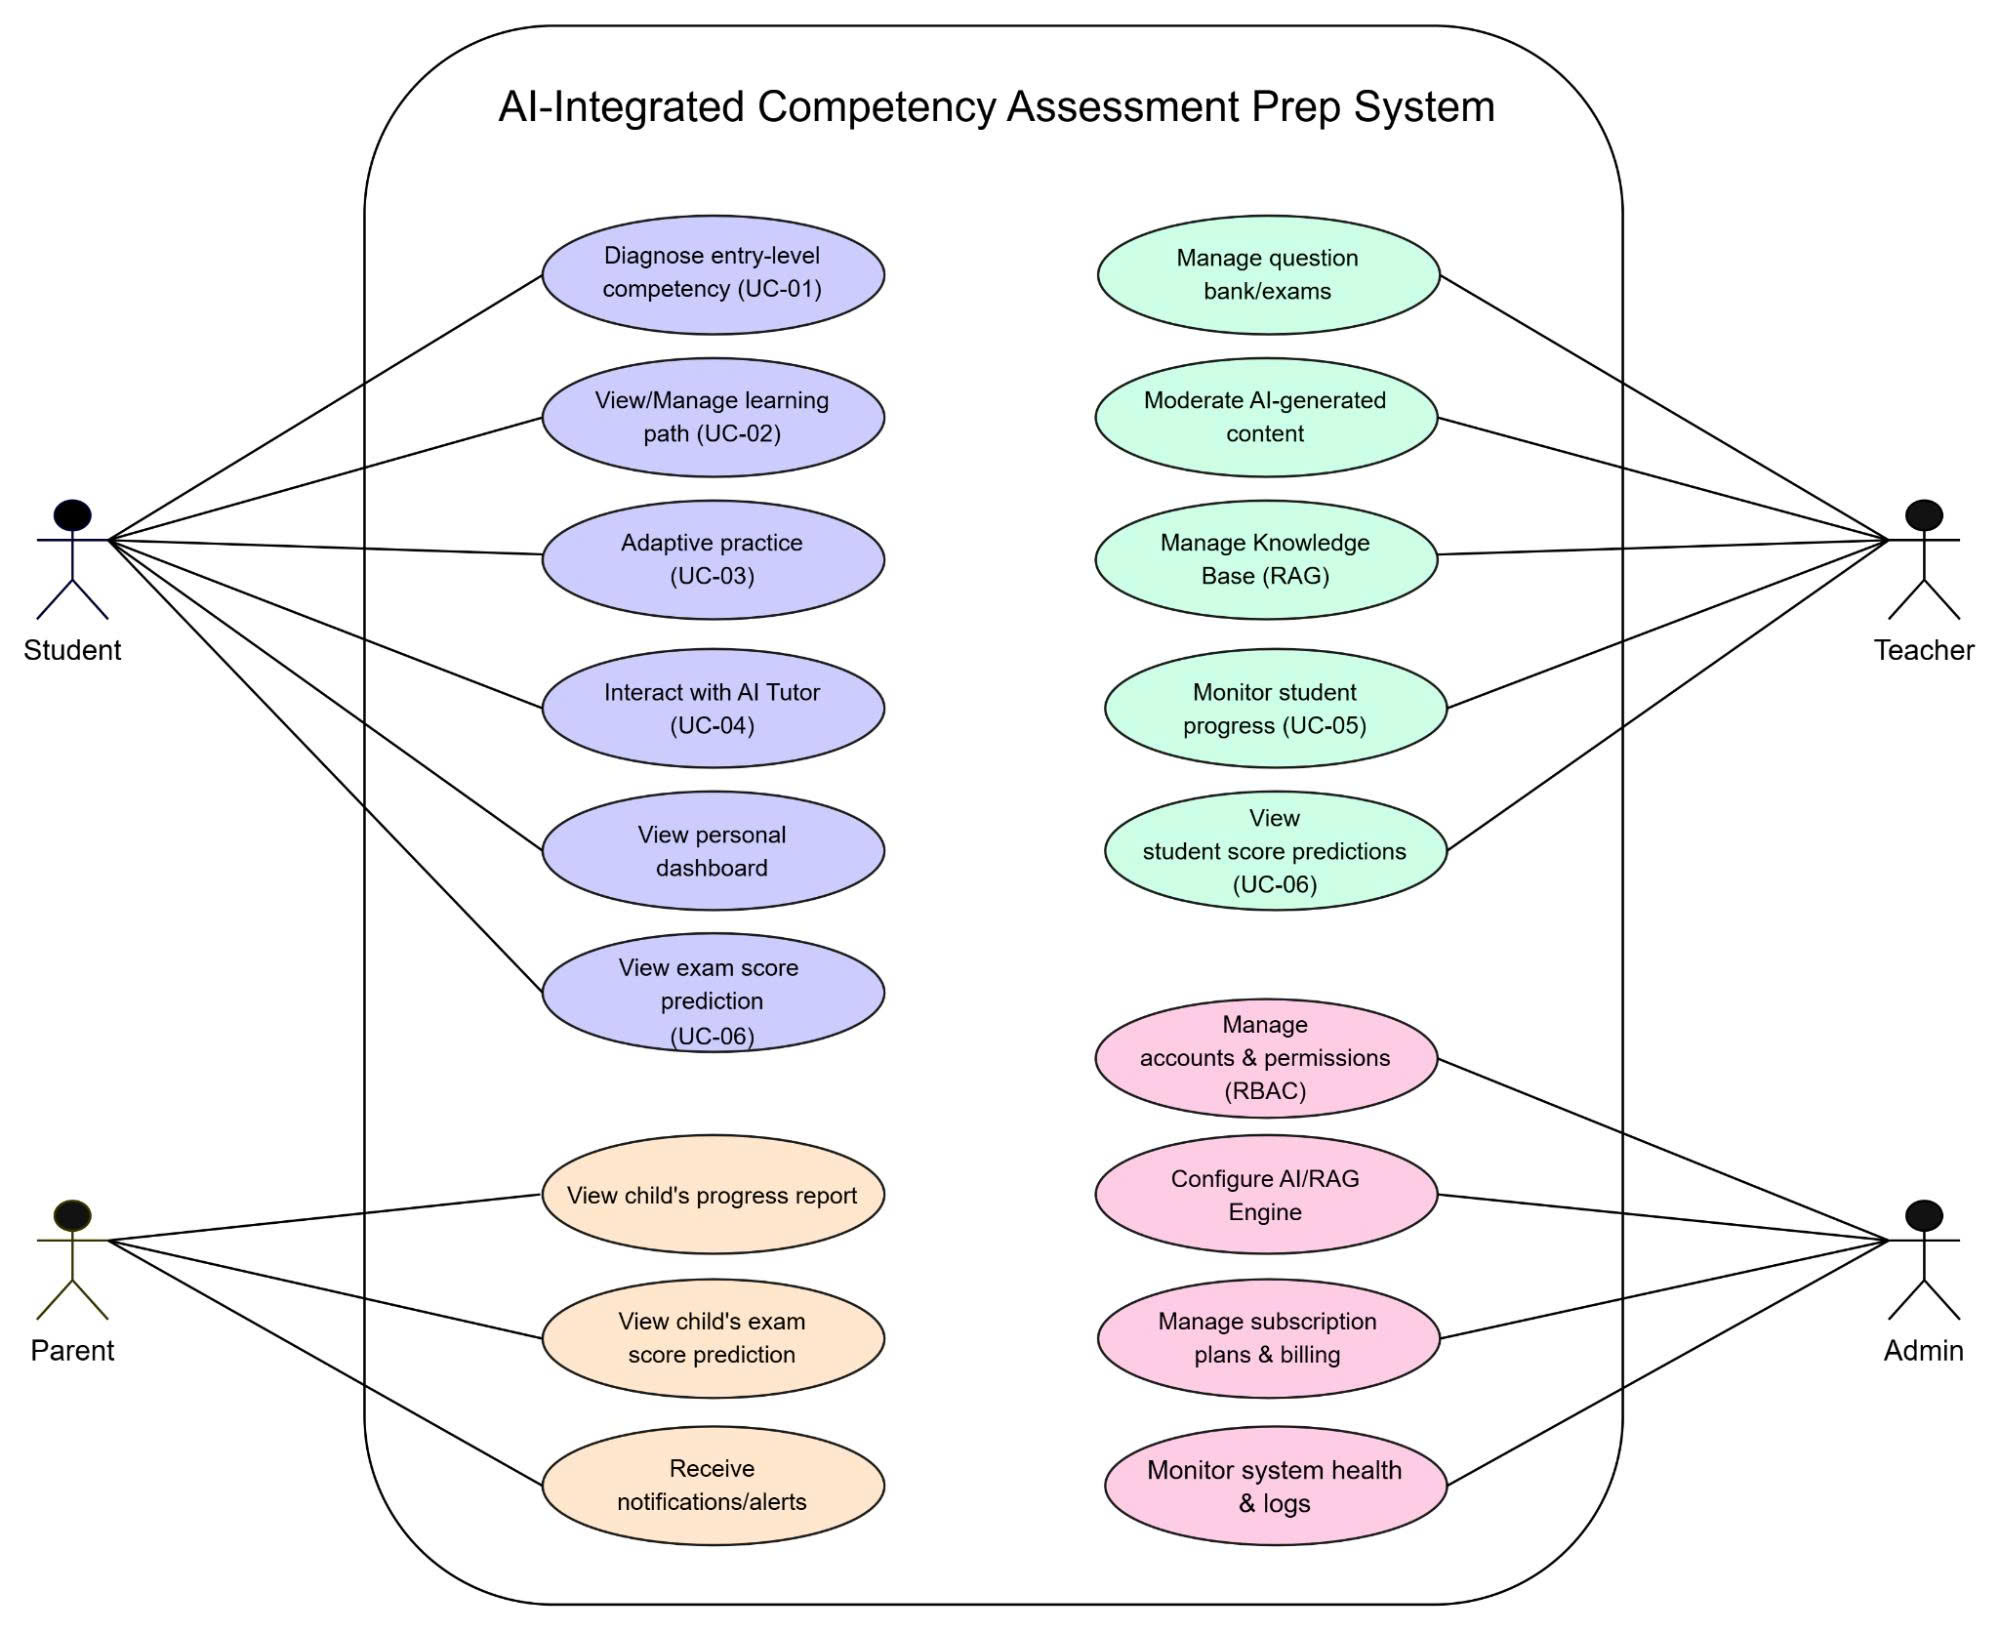
\includegraphics[width=0.9\textwidth]{figure_sdd_overall_use_case.png}
    \caption{Overall System Use Case Diagram}
    \label{fig:sdd_overall_use_case}
\end{figure}

\subsubsection{Student \& AI Interactive Use Case Diagram}
This diagram details the core interactive workflows for the Student actor, encompassing diagnostic assessment (UC-01), roadmap generation (UC-02), real-time adaptive practice loops (UC-03), RAG-powered AI Tutor interactions (UC-04), personal dashboards (UC-05), and predicted exam scores (UC-06).

\begin{figure}[H]
    \centering
    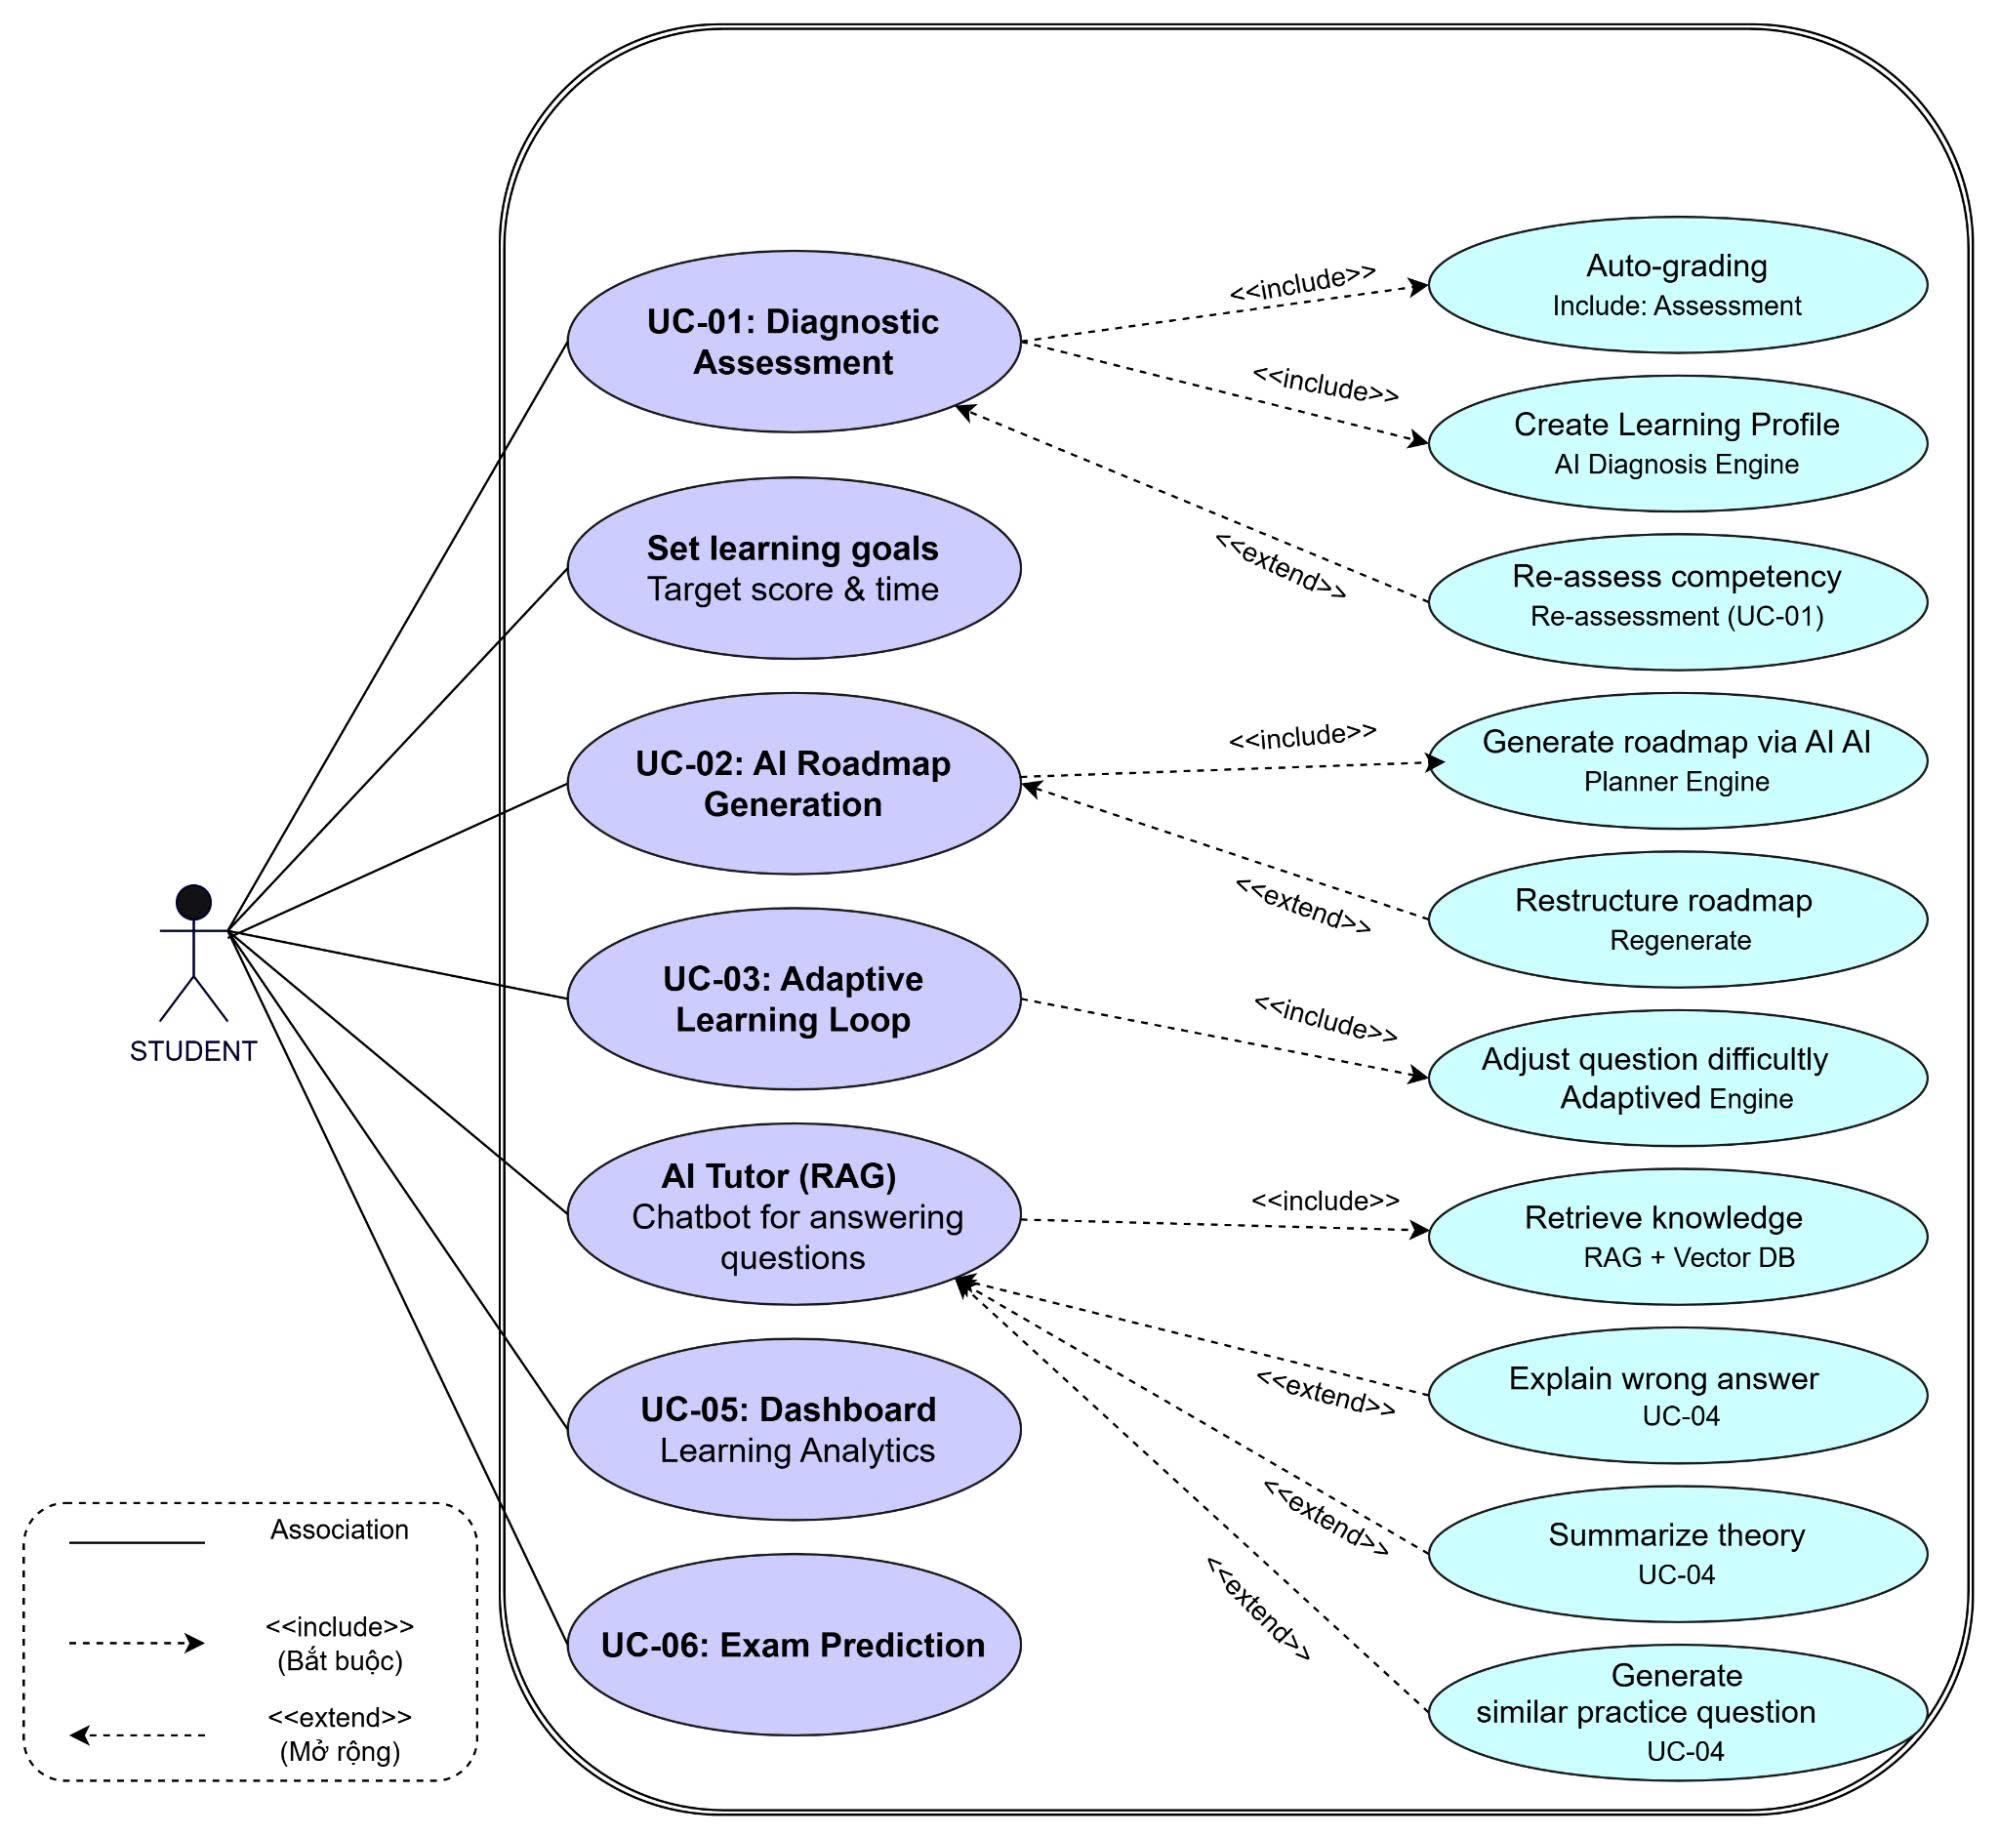
\includegraphics[width=0.9\textwidth]{figure_sdd_student_use_case.png}
    \caption{Student \& AI Interactive Use Case Diagram}
    \label{fig:sdd_student_use_case}
\end{figure}

\subsubsection{Teacher \& Admin Use Case Diagram}
This detailed diagram depicts administrative and academic management functions. System Administrators configure AI parameters, RBAC roles, and system security. Teachers manage standardized question banks, upload educational documents to the Vector Database, and moderate AI-generated responses (Human-in-the-loop).

\begin{figure}[H]
    \centering
    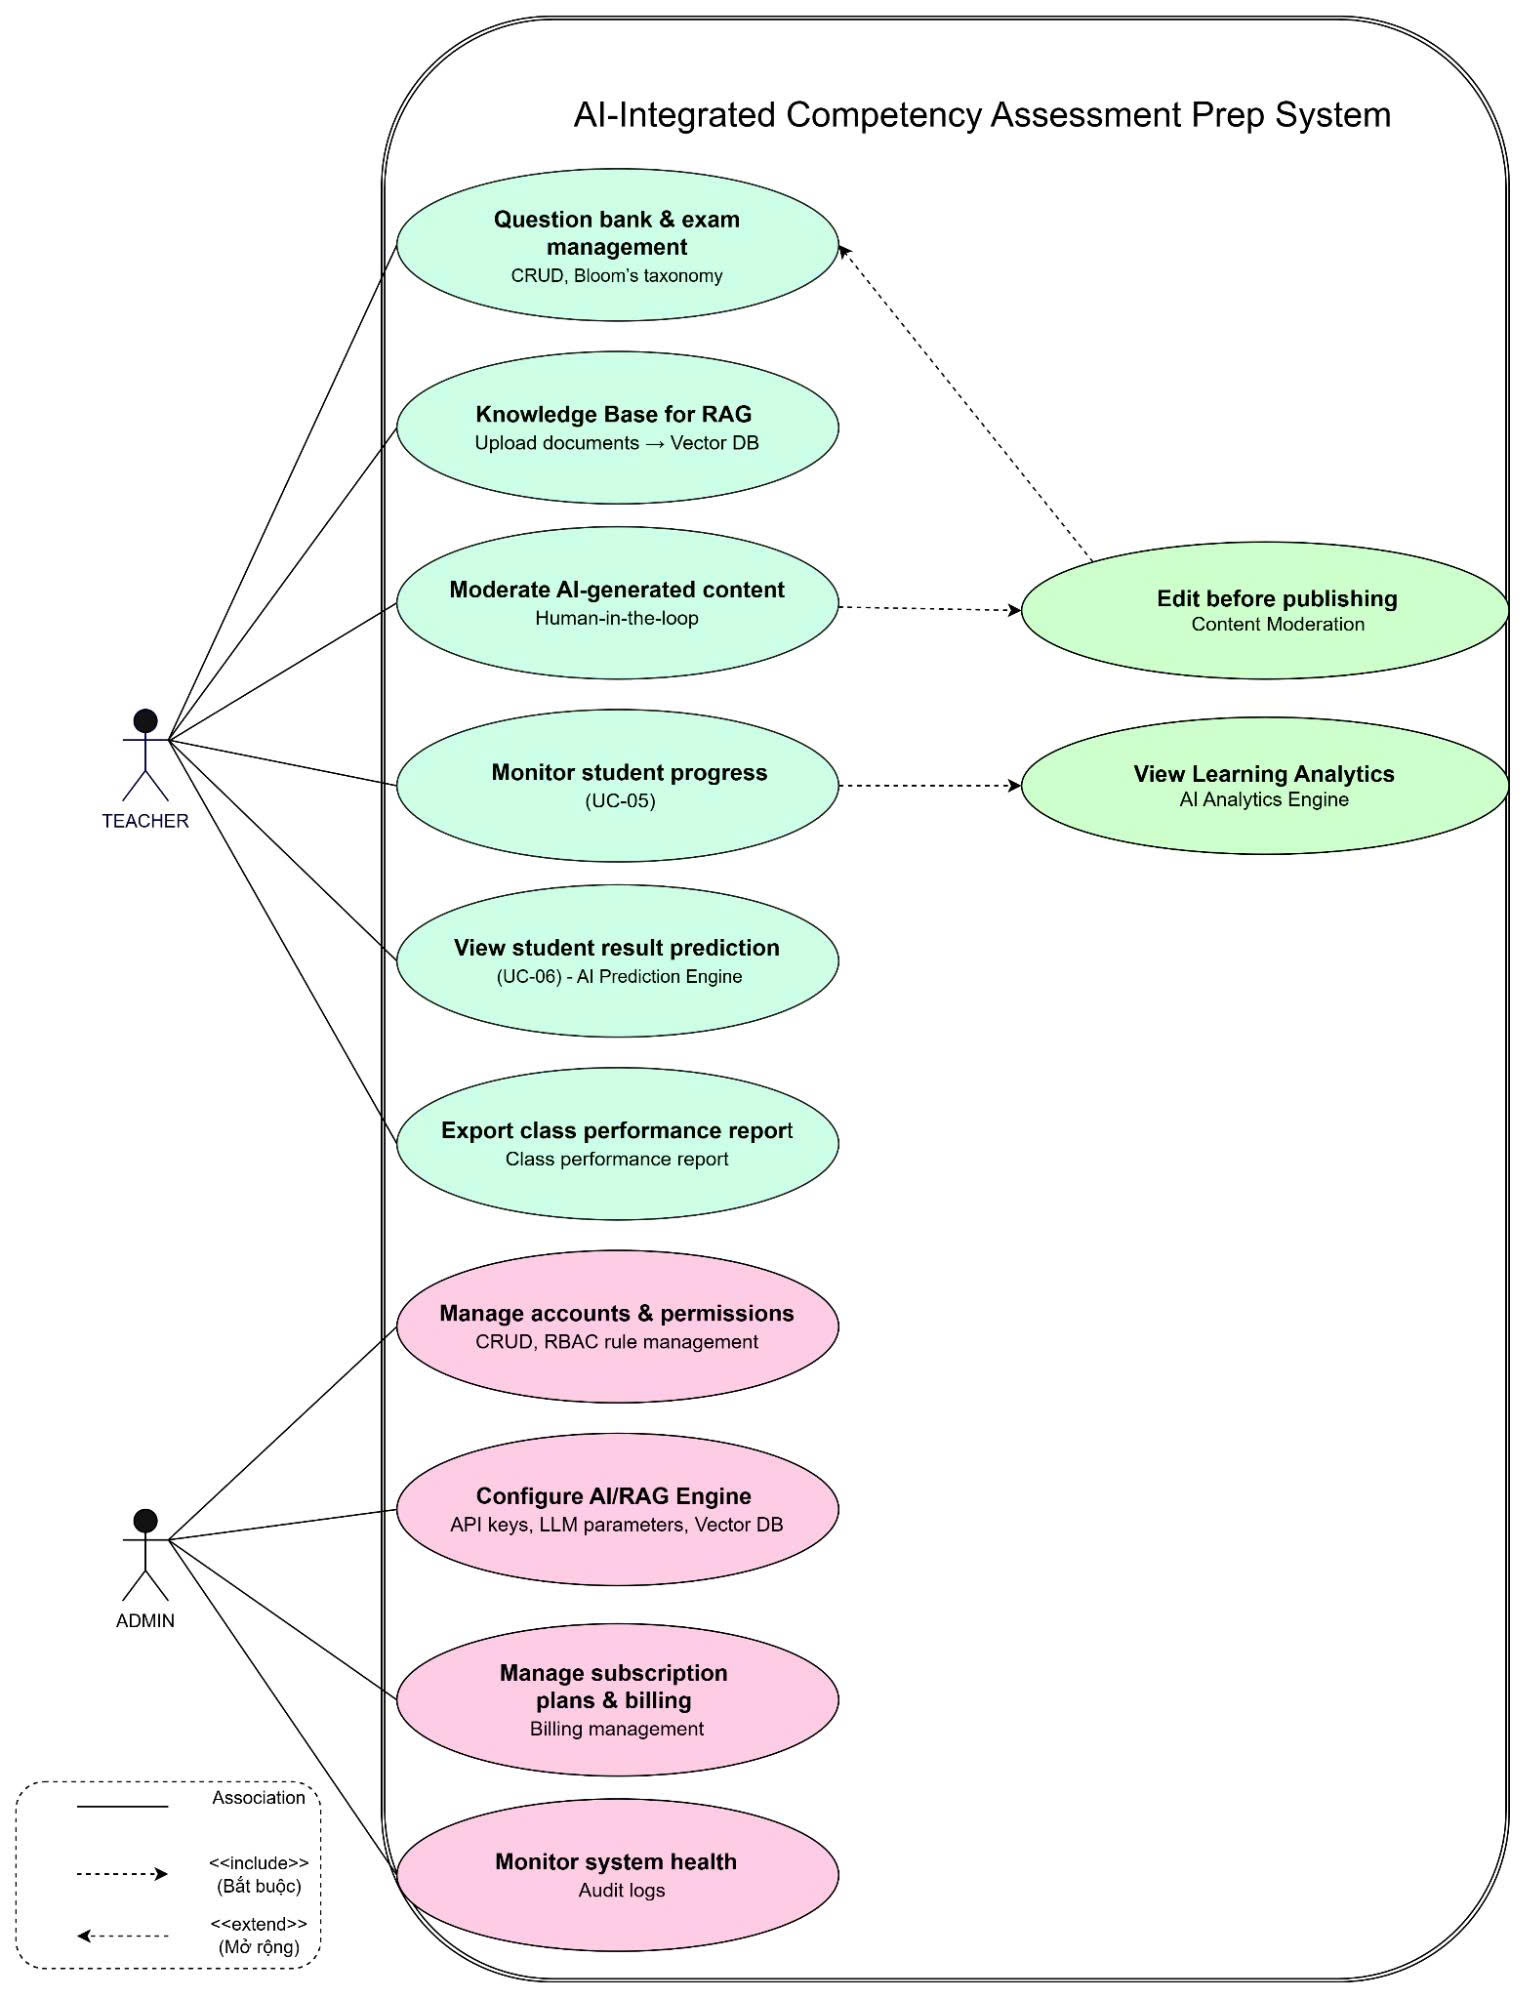
\includegraphics[width=0.9\textwidth]{figure_sdd_teacher_admin_use_case.png}
    \caption{Teacher \& Admin Use Case Diagram}
    \label{fig:sdd_teacher_admin_use_case}
\end{figure}

\subsubsection{Parent Use Case Diagram}
This diagram outlines the read-only monitoring functionalities for Parent accounts, including progress tracking, attendance/inactivity alerts, and automated performance reports.

\begin{figure}[H]
    \centering
    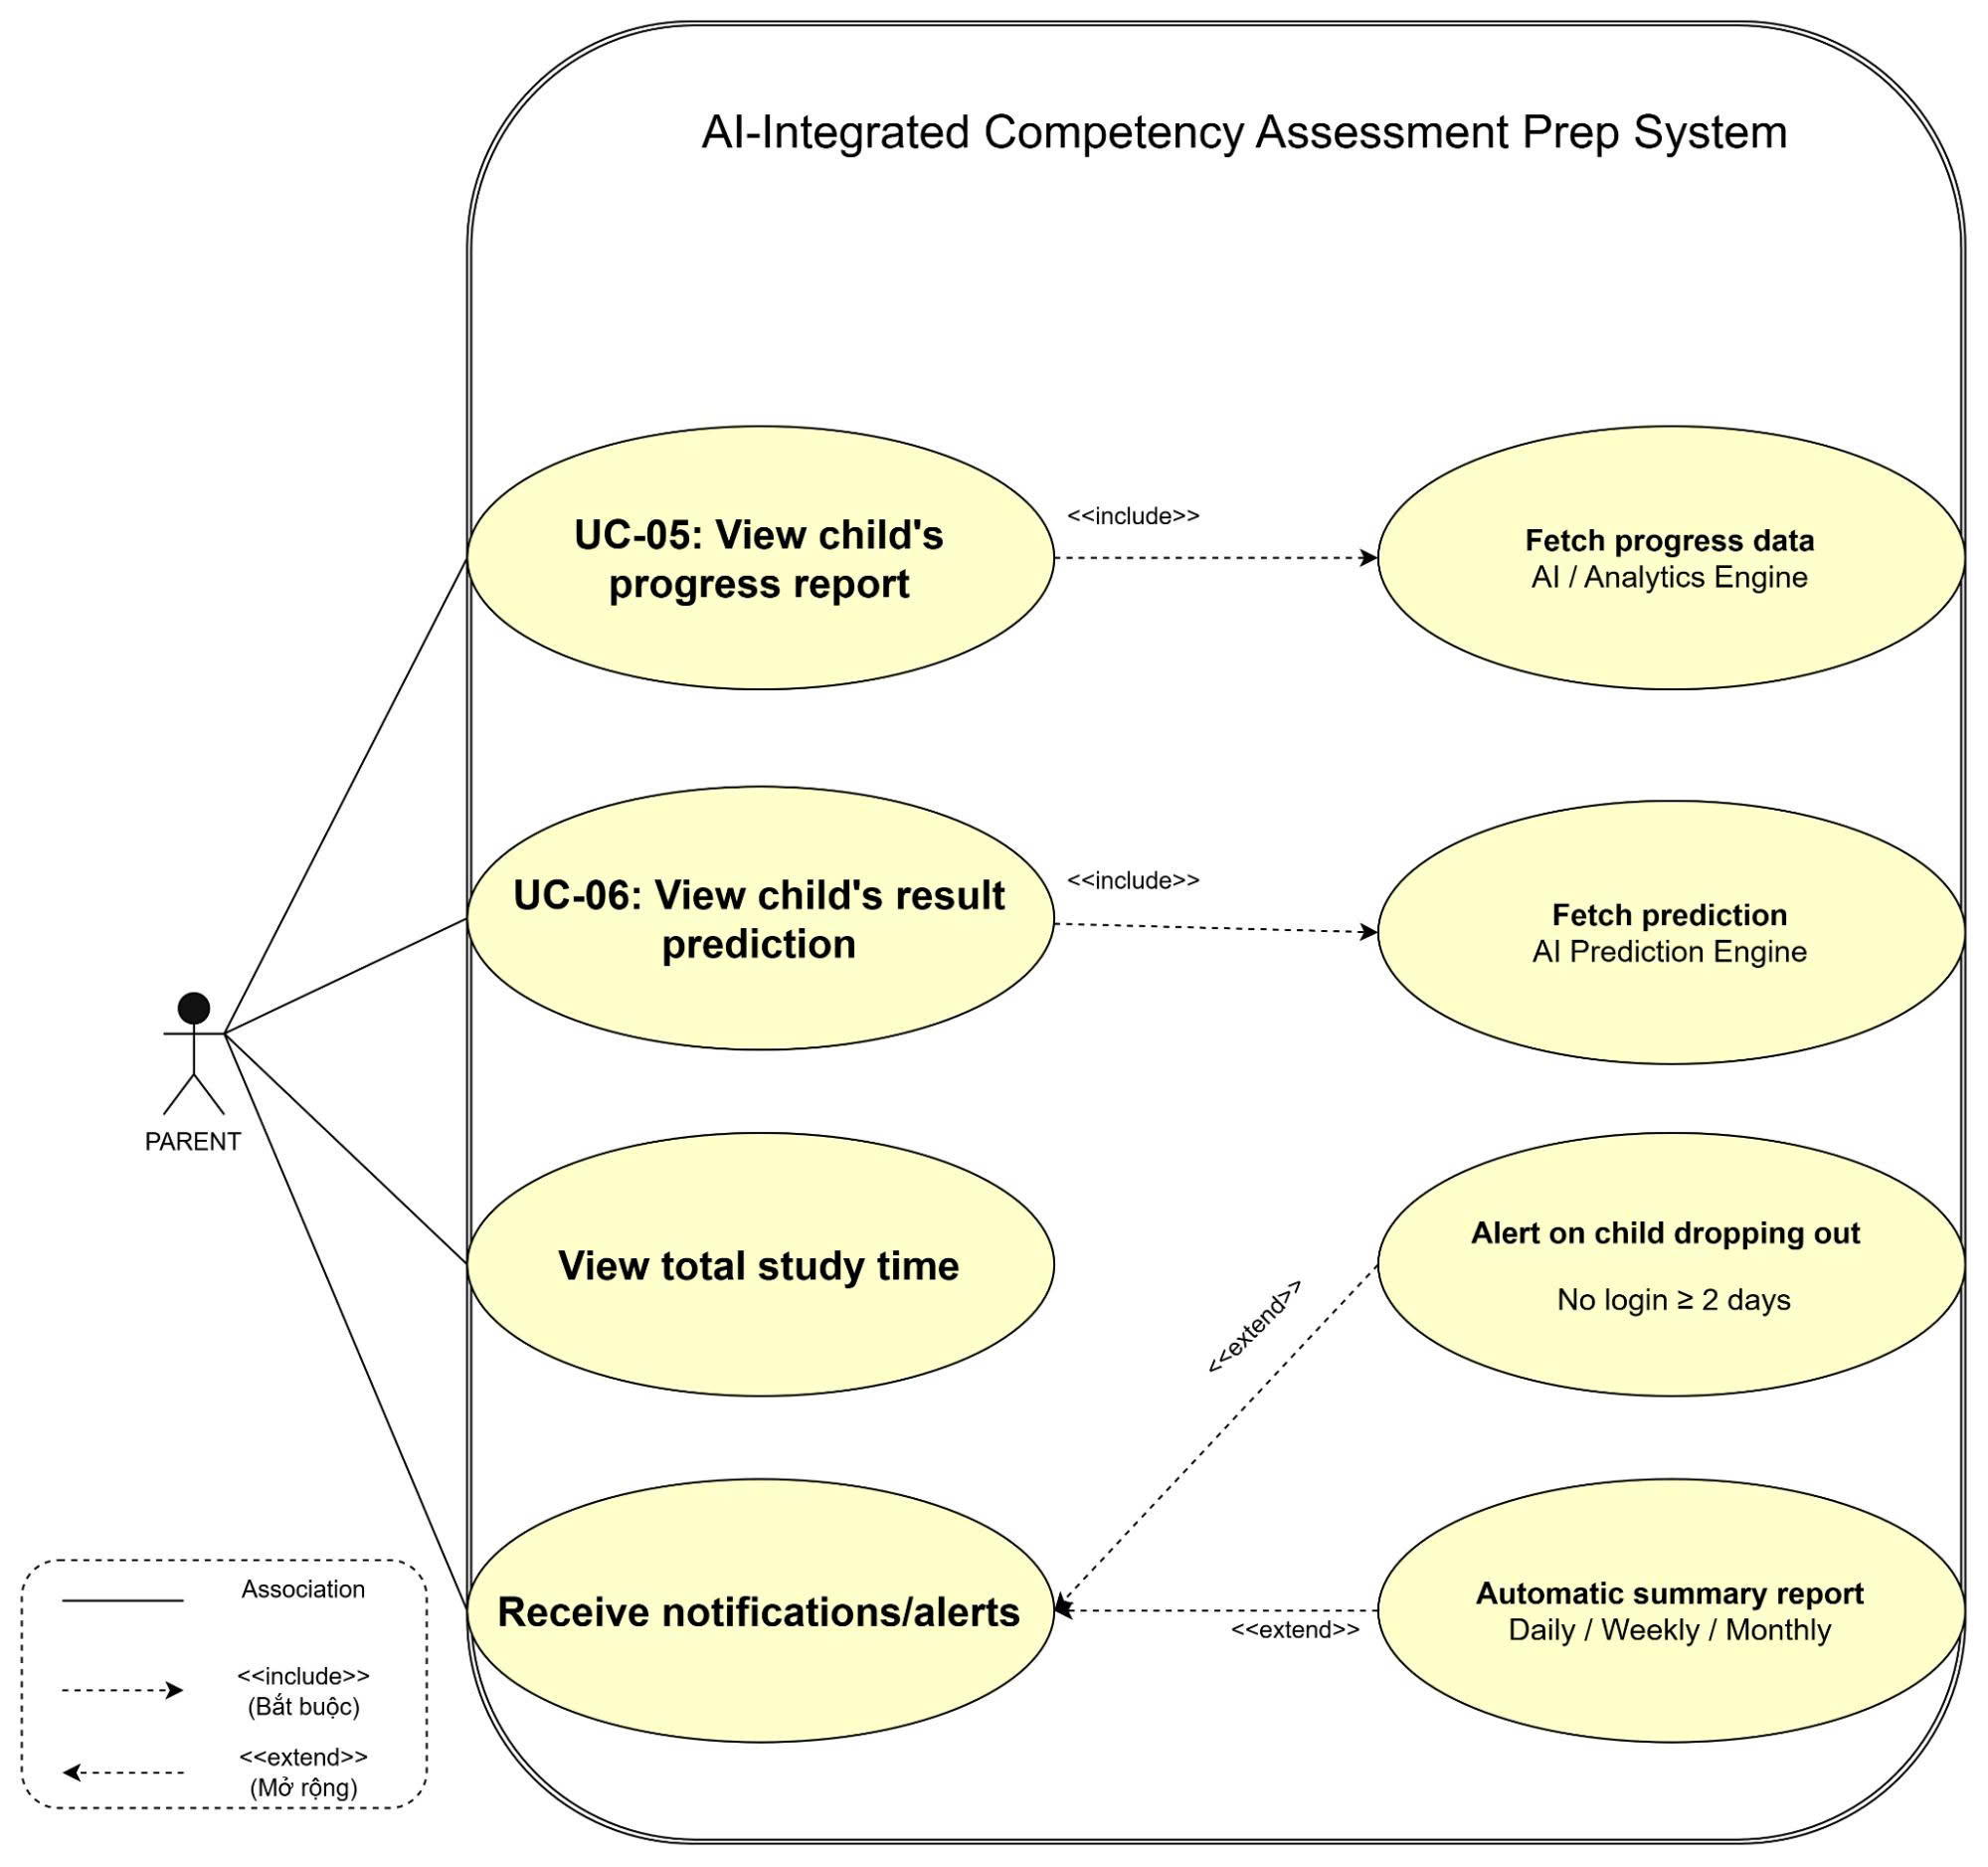
\includegraphics[width=0.82\textwidth]{figure_sdd_parent_use_case.png}
    \caption{Parent Use Case Diagram}
    \label{fig:sdd_parent_use_case}
\end{figure}

\subsection{Database Design (ERD \& Vector DB)}

\subsubsection{Relational Database Schema (ERD)}
The relational database manages operational data including Users, Roles, Question Banks, Diagnostic Sessions, Learning Profiles, and Roadmap Daily Tasks. Strict foreign key constraints and index optimizations ensure data integrity and fast response times ($< 3.0$s).

\subsubsection{Vector Database Architecture \& AI RAG Pipeline}
The system utilizes an in-memory / relational vector store for baseline semantic retrieval. Textbooks and solution documents are processed into chunks and stored in the \texttt{vector\_chunks} table:
\begin{itemize}[leftmargin=1.5em, itemsep=0.2em]
    \item \texttt{chunk\_id} (UUID, Primary Key): Unique identifier for each text chunk.
    \item \texttt{document\_id} (String, Foreign Key): Identifier of the original source document.
    \item \texttt{text\_content} (Text): Raw textual context extracted from documents.
    \item \texttt{embedding\_vector} (Array[Float]): Dense L2-normalized vector array.
    \item \texttt{chunk\_index} (Integer): Sequence position of the chunk in the document.
\end{itemize}

\subsubsection{AI RAG Processing Algorithms}
\begin{itemize}[leftmargin=1.5em, itemsep=0.2em]
    \item \textbf{Text Chunker (\texttt{text\_chunker}):} Splits source documents using a sliding window algorithm with a default \texttt{chunk\_size} of 100 words and an overlap of 20 words.
    \item \textbf{Vector Embedding \& L2 Normalization (\texttt{generate\_embedding}):} Converts plain text into numeric vectors and scales them to unit length ($\|v\|=1.0$) for optimized vector operations.
    \item \textbf{Cosine Similarity \& Top-K Retrieval (\texttt{retrieve\_relevant\_chunks}):} Computes angular similarity between user query vectors and chunk vectors to retrieve the Top-K ($K=3$) most relevant contexts for the AI Tutor.
\end{itemize}

\subsection{Sequence Diagrams \& Detailed Design}
Sequence diagrams describe the chronological object interactions across the Frontend, Backend API Gateway, IRT Engine, RAG Service, Vector DB, and LLM API for critical business flows:
\begin{itemize}[leftmargin=1.5em, itemsep=0.2em]
    \item \textbf{SD-01:} Real-time Item Response Adjustment during Adaptive Practice (UC-03).
    \item \textbf{SD-02:} RAG Context Retrieval and Streaming Response Generation for AI Tutor Chatbot (UC-04).
\end{itemize}

\begin{figure}[H]
    \centering
    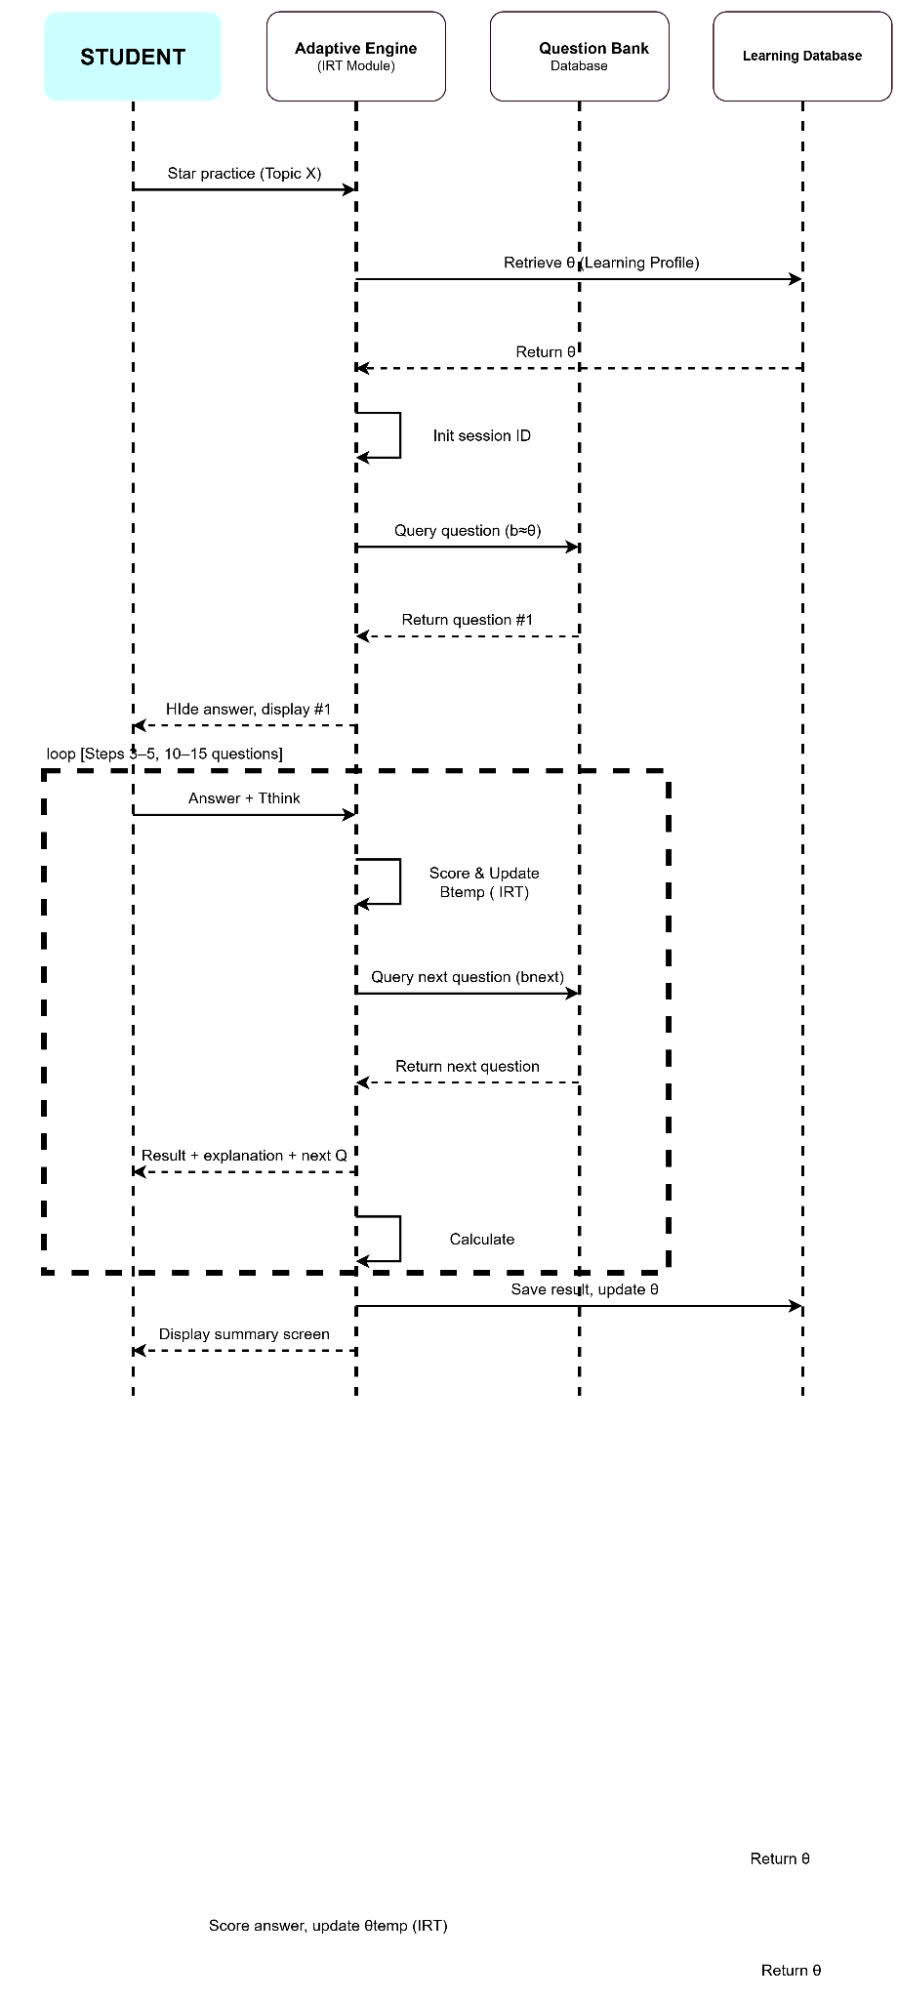
\includegraphics[width=0.9\textwidth,height=0.9\textheight,keepaspectratio]{figure_sd01_adaptive.png}
    \caption{SD-01: Real-time Item Response Adjustment during Adaptive Practice (UC-03)}
    \label{fig:sd01_adaptive}
\end{figure}

\begin{figure}[H]
    \centering
    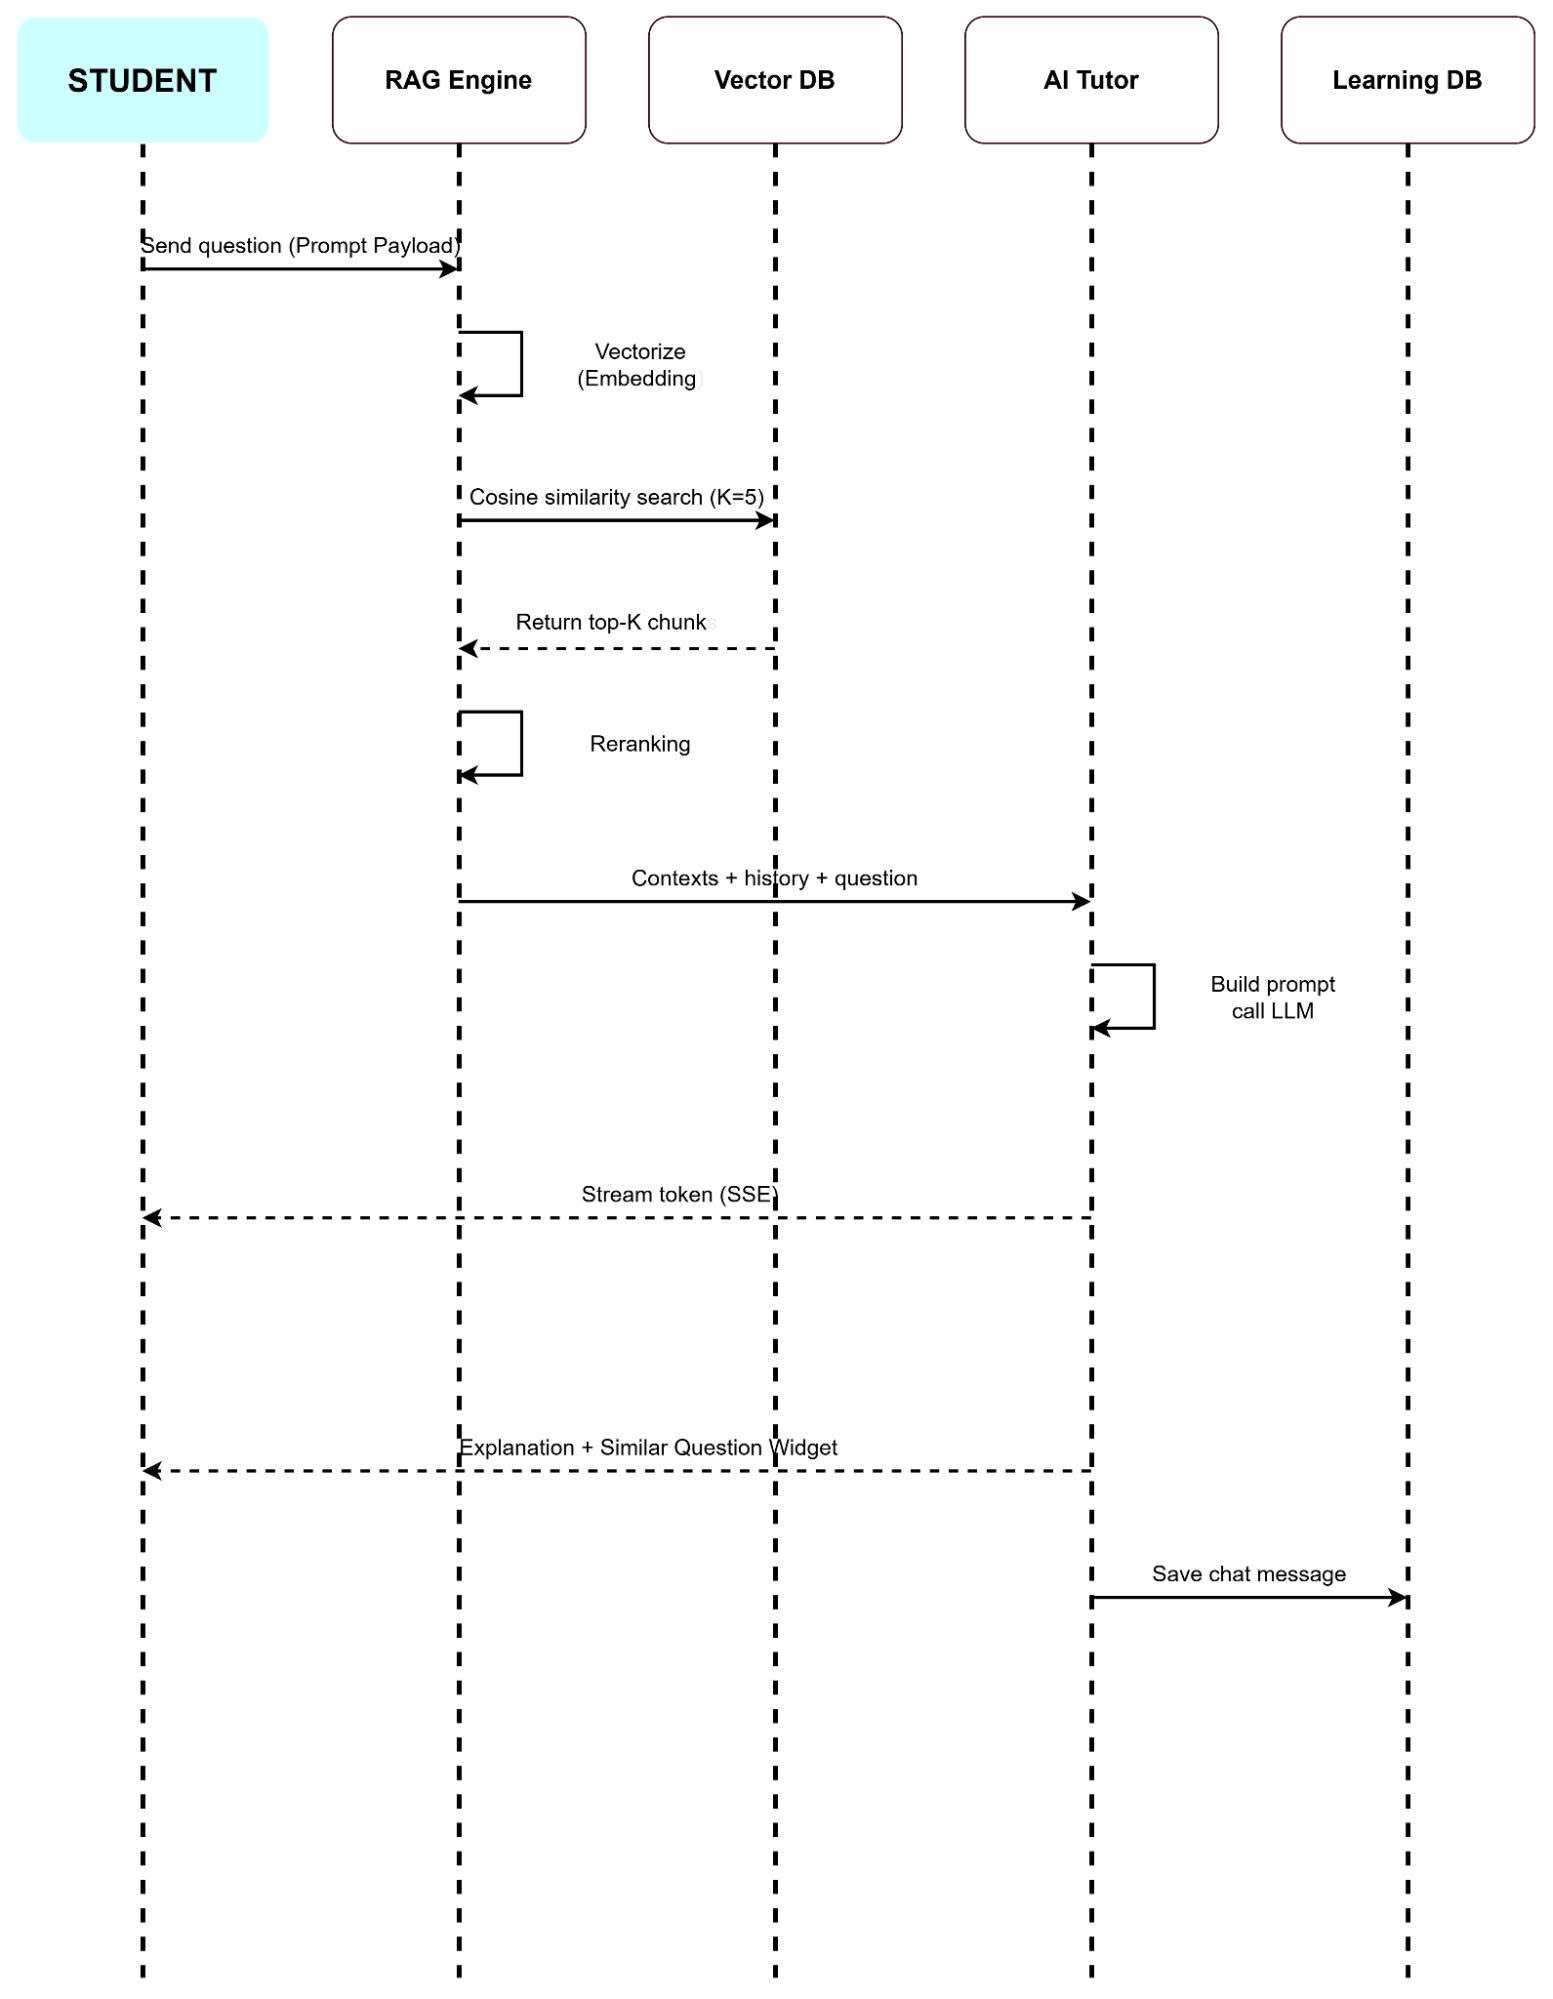
\includegraphics[width=0.85\textwidth,height=0.8\textheight,keepaspectratio]{figure_sd02_rag.png}
    \caption{SD-02: RAG Context Retrieval and Streaming Response Generation for AI Tutor Chatbot (UC-04)}
    \label{fig:sd02_rag}
\end{figure}

\section{System Implementation \& Testing}

\subsection{Implementation Tech Stack}
\begin{itemize}[leftmargin=1.5em, itemsep=0.2em]
    \item \textbf{Backend Core:} Python 3.10+, FastAPI framework, SQLAlchemy ORM (async/sync sessions), Pydantic v2 data validation schemas.
    \item \textbf{Security \& Authentication:} JWT Bearer Token Authentication (HS256), Bcrypt cryptographic password hashing, Role-Based Access Control (RBAC) dependency injection middleware.
    \item \textbf{Database \& Storage:} PostgreSQL / Supabase for relational operational persistence; in-memory vector embeddings with Cosine Similarity for RAG retrieval.
    \item \textbf{Artificial Intelligence Engine:} Google Gemini API (gemini-1.5-flash) integrated via asynchronous streaming with Socratic pedagogical system prompts.
    \item \textbf{Frontend Application:} React.js 19, Vite build tool, Material-UI (MUI v7), React Router v7, KaTeX math typesetting engine (rehype-katex, remark-math).
    \item \textbf{Automated Testing Suite:} Pytest testing framework with isolated SQLite test database fixtures and unittest.mock asynchronous stubs.
\end{itemize}

\subsection{System Features \& User Interface Walkthrough}

\subsubsection{Authentication \& Multi-Role Access Control (RBAC)}
\begin{itemize}[leftmargin=1.5em, itemsep=0.2em]
    \item \textbf{Functional Description:} Serves as the primary security gateway for the platform. It enforces distinct operational boundaries across the four primary system personas: Student, Teacher, Parent, and System Administrator.
    \item \textbf{User Workflow \& Validation Rules:}
    \begin{enumerate}[leftmargin=1.5em, itemsep=0.1em]
        \item Users access the unified authentication screen at \texttt{/login}.
        \item The form validates email formatting via RFC-compliant regex and mandates a minimum password length of 8 characters.
        \item Upon successful credential verification, the backend issues an \texttt{access\_token} (30-minute lifespan) and a \texttt{refresh\_token} (7-day lifespan).
        \item The frontend context automatically decodes user role claims and routes the client to the appropriate workspace (\texttt{/student}, \texttt{/teacher}, \texttt{/parent}, or \texttt{/admin}).
    \end{enumerate}
    \item \textbf{Underlying APIs:} \texttt{POST /api/v1/auth/register}, \texttt{POST /api/v1/auth/login}, \texttt{GET /api/v1/auth/me}.
\end{itemize}

\begin{figure}[H]
    \centering
    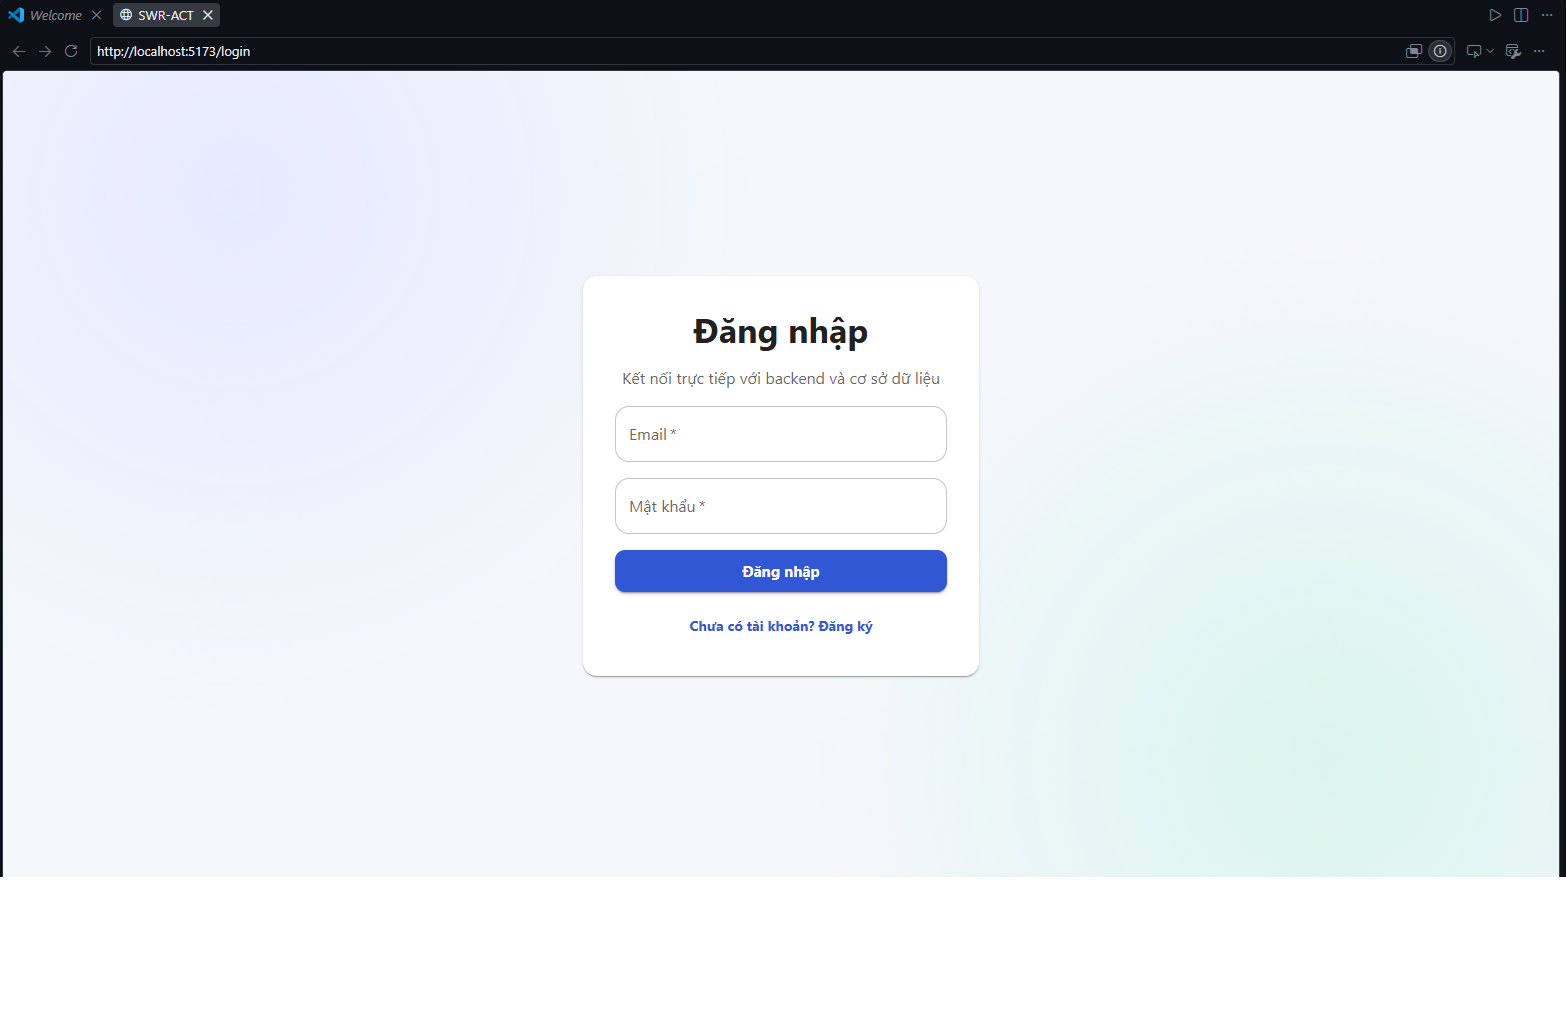
\includegraphics[width=1\textwidth]{figure_5_1_login.png}
    \caption{User Authentication and Role-Based Redirection Interface}
    \label{fig:ui_login}
\end{figure}

\subsubsection{Competency Diagnosis \& Baseline Assessment Module (UC-01)}
\begin{itemize}[leftmargin=1.5em, itemsep=0.2em]
    \item \textbf{Functional Description:} Evaluates the student's baseline academic capability across multiple knowledge domains (Mathematics, Logic Reasoning, Vietnamese Language) to identify existing knowledge gaps before generating a study plan.
    \item \textbf{User Workflow \& UI Components:}
    \begin{enumerate}[leftmargin=1.5em, itemsep=0.1em]
        \item The student initiates a diagnostic session via \texttt{/student/assessment}.
        \item The system loads 15 standardized competency evaluation items into an interactive examination room.
        \item A real-time countdown timer (15:00 minutes) and linear progress bar dynamically track examination progress.
        \item Mathematical expressions and equations are rendered natively using KaTeX.
        \item Upon submission (manual or auto-submitted upon timer expiration), the system calculates raw score metrics and presents a granular review showing selected options, correct keys, and comprehensive explanations.
    \end{enumerate}
    \item \textbf{Underlying APIs:} \texttt{GET /api/diagnostic/questions}, \texttt{POST /api/diagnostic/submit}.
\end{itemize}

\begin{figure}[H]
    \centering
    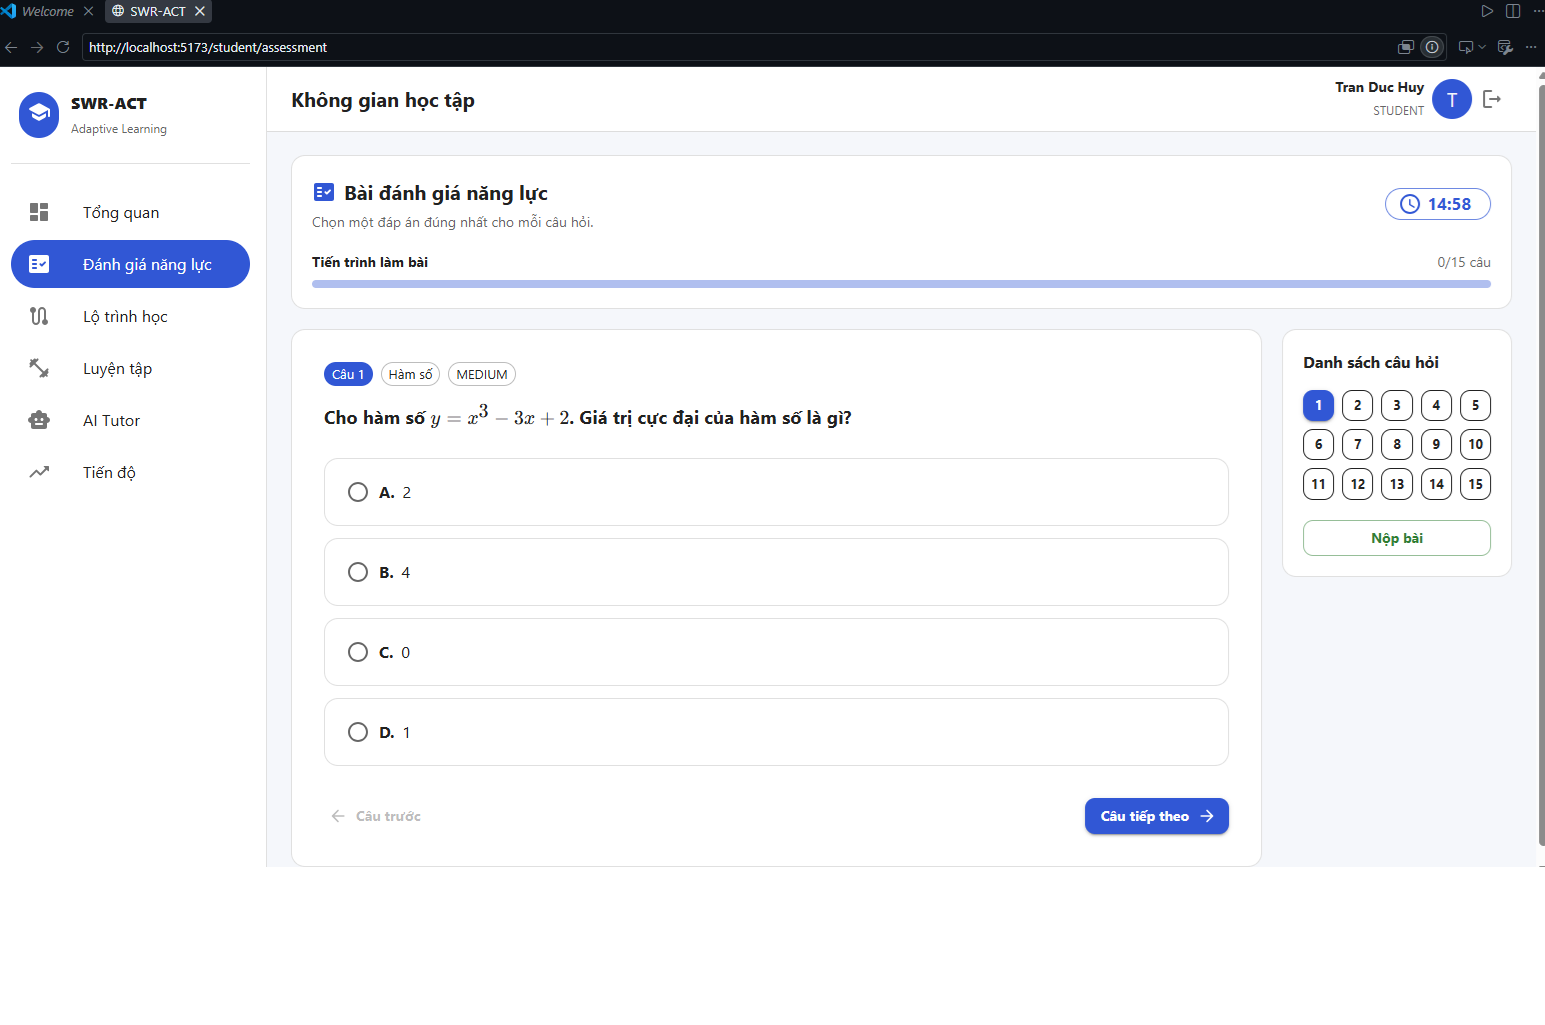
\includegraphics[width=1\textwidth]{figure_5_2_assessment.png}
    \caption{Diagnostic Assessment Exam Room with KaTeX Math Rendering and Countdown Timer}
    \label{fig:ui_assessment}
\end{figure}

\begin{figure}[H]
    \centering
    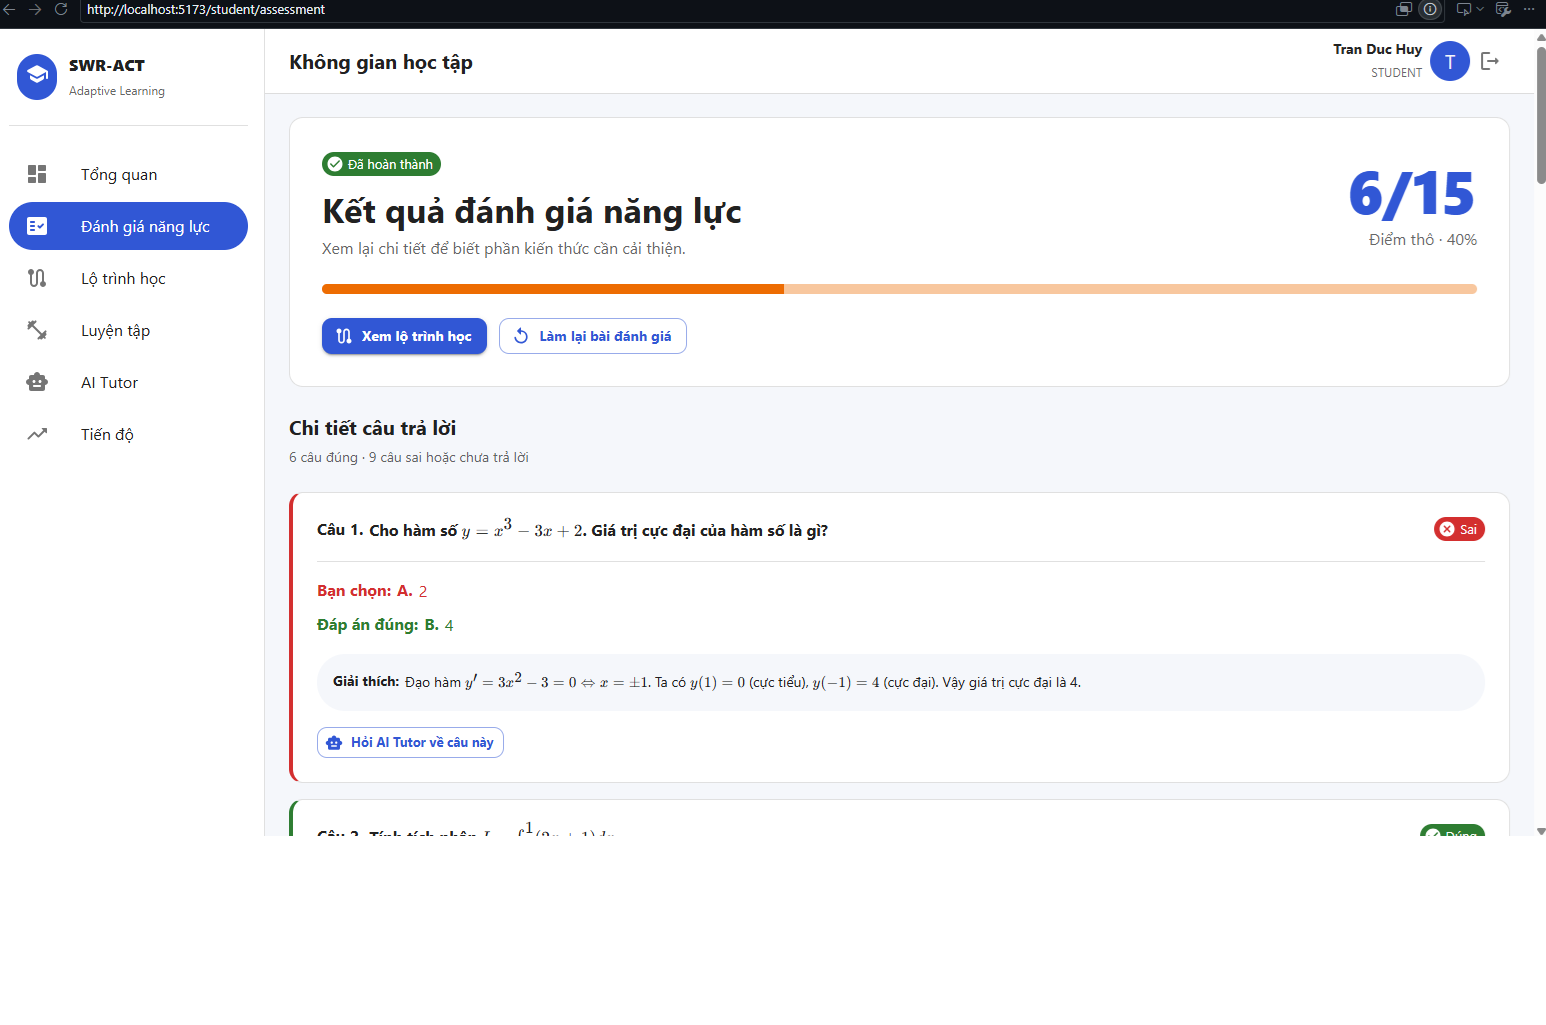
\includegraphics[width=1\textwidth]{figure_5_3_summary.png}
    \caption{Diagnostic Evaluation Summary and Detailed Explanations View}
    \label{fig:ui_diagnostic_summary}
\end{figure}

\subsubsection{Goal Setting \& Personalized Learning Roadmap Module (UC-02)}
\begin{itemize}[leftmargin=1.5em, itemsep=0.2em]
    \item \textbf{Functional Description:} Converts diagnostic test outcomes into actionable, daily study milestones customized to the student's target competency score and preparation timeframe.
    \item \textbf{User Workflow \& UI Components:}
    \begin{enumerate}[leftmargin=1.5em, itemsep=0.1em]
        \item The student accesses the roadmap screen at \texttt{/student/roadmap} and opens the Goal Setup Modal.
        \item Input constraints are validated in real-time:
        \begin{itemize}[leftmargin=1.2em]
            \item Target Score ($S_{\text{target}}$): Range 1 to 1200 points.
            \item Exam Date ($D_{\text{exam}}$): Must be a valid future date.
            \item Daily Study Time ($T_{\text{daily}}$): Range 0.5 to 12.0 hours/day.
        \end{itemize}
        \item The backend calculates total remaining preparation days and initializes a structured 4-phase learning trajectory stored in \texttt{study\_plans} and \texttt{plan\_tasks}.
    \end{enumerate}
    \item \textbf{Underlying APIs:} \texttt{POST /api/study-plan/init}.
\end{itemize}

\begin{figure}[H]
    \centering
    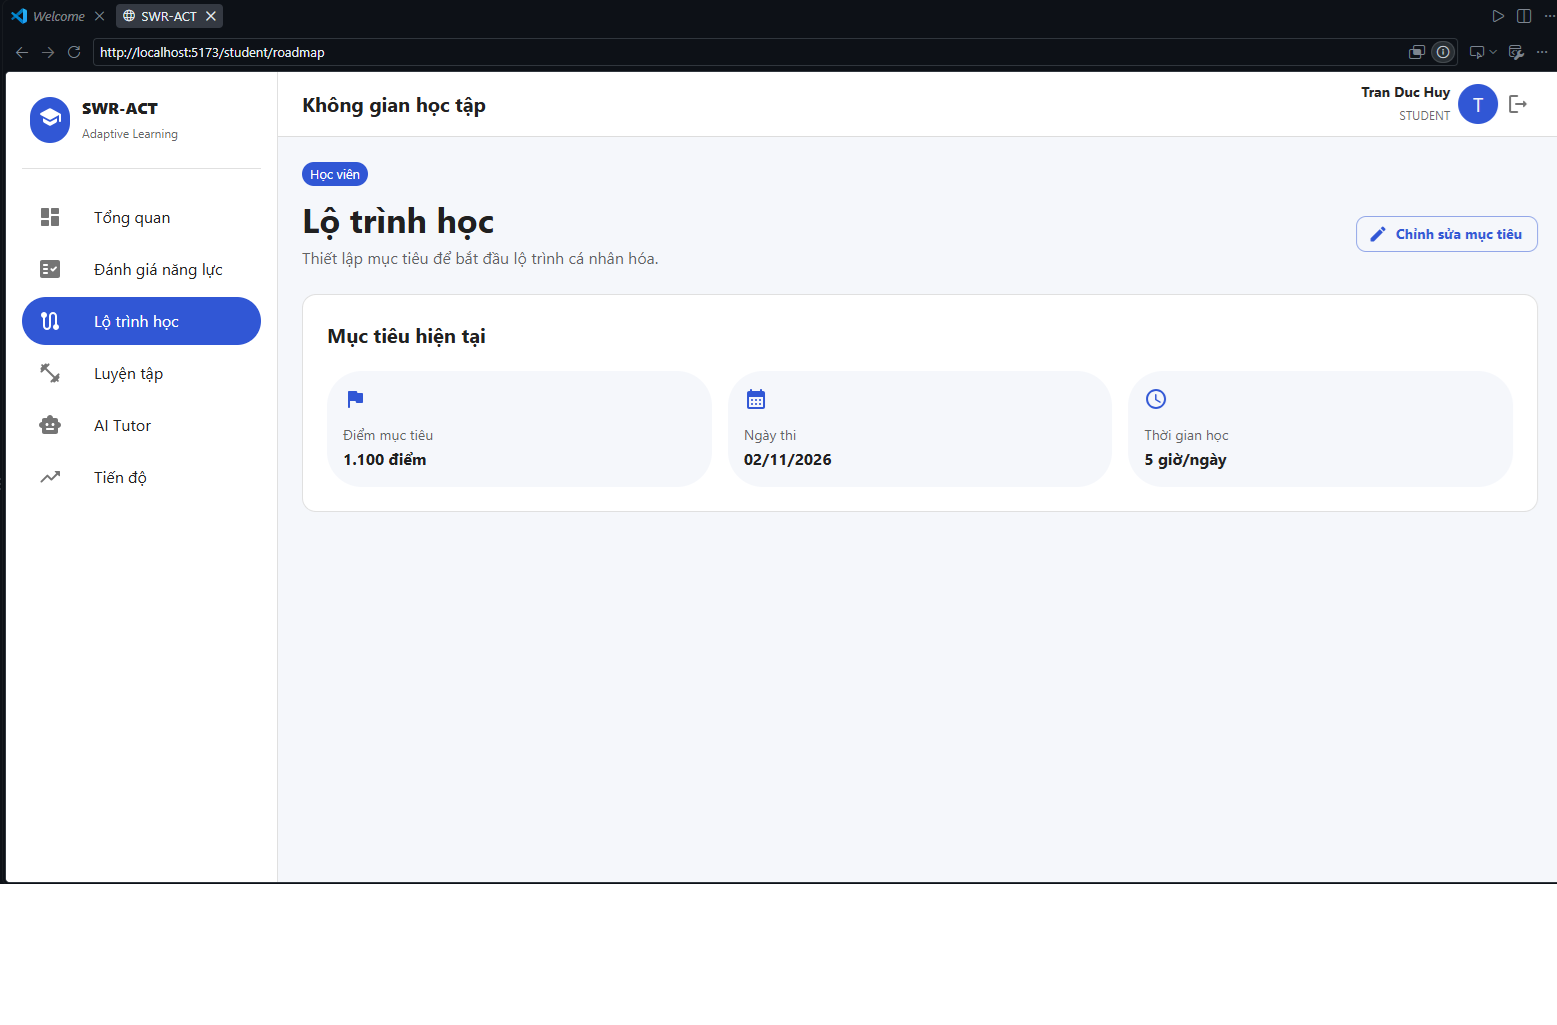
\includegraphics[width=1\textwidth]{figure_5_4_roadmap.png}
    \caption{Goal Setup Modal and Active Milestone Trajectory Dashboard}
    \label{fig:ui_roadmap}
\end{figure}

\subsubsection{Topic-Based Adaptive Practice Module (UC-03)}
\begin{itemize}[leftmargin=1.5em, itemsep=0.2em]
    \item \textbf{Functional Description:} Allows students to engage in targeted practice sessions filtered by specific subject areas, topic clusters, and difficulty tiers to reinforce weak competencies.
    \item \textbf{User Workflow \& UI Components:}
    \begin{enumerate}[leftmargin=1.5em, itemsep=0.1em]
        \item The student configures a session on the Practice page by selecting:
        \begin{itemize}[leftmargin=1.2em]
            \item Subject: Toan hoc , Logic , Tieng Viet
            \item Topic: Ham so , tinh phan , menh de , ...
            \item Difficulty: EASY, MEDIUM, HARD.
        \end{itemize}
        \item The system retrieves matched question items from the database.
        \item The exam room provides a numeric question navigator grid, allowing students to track answered/unanswered questions seamlessly.
        \item Post-submission results persist into \texttt{tests} and \texttt{user\_answers}, generating a performance breakdown with a dedicated ``Hoi AI cau nay'' (Ask AI Tutor) button next to every incorrect answer.
    \end{enumerate}
    \item \textbf{Underlying APIs:} \texttt{GET /api/practice/questions}, \texttt{POST /api/practice/submit}, \texttt{GET /api/practice/history}.
\end{itemize}

\begin{figure}[H]
    \centering
    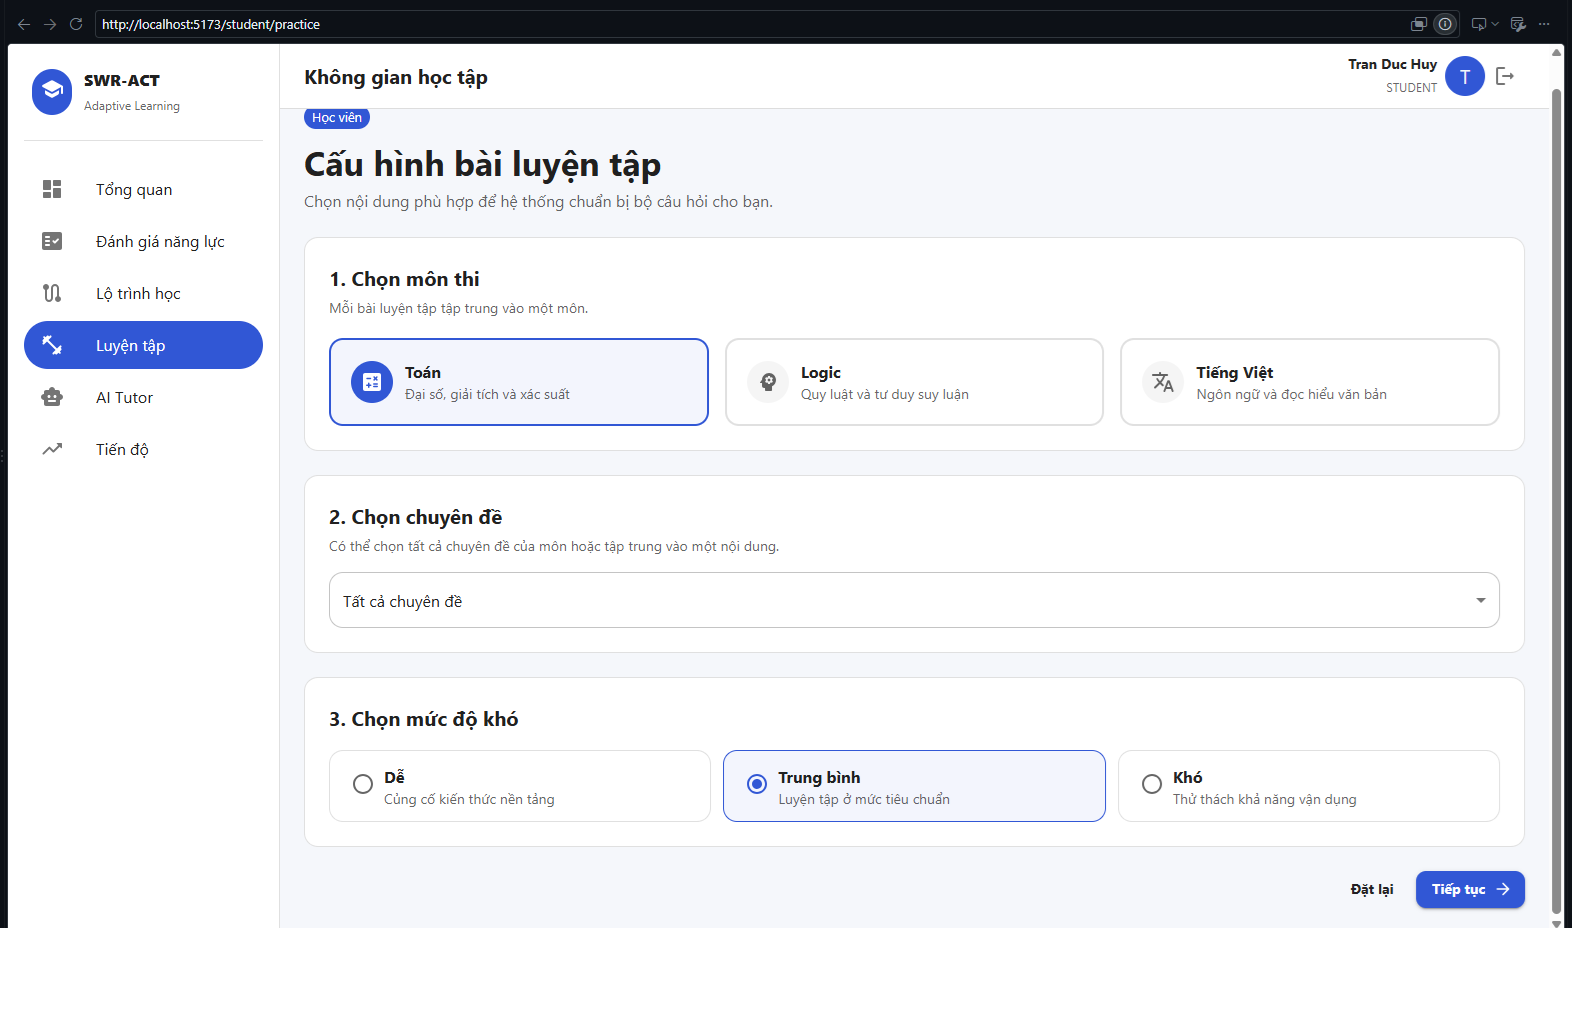
\includegraphics[width=1\textwidth]{figure_5_5_practice_config.png}
    \caption{Topic and Difficulty Configuration for Adaptive Practice Sessions}
    \label{fig:ui_practice_config}
\end{figure}

\begin{figure}[H]
    \centering
    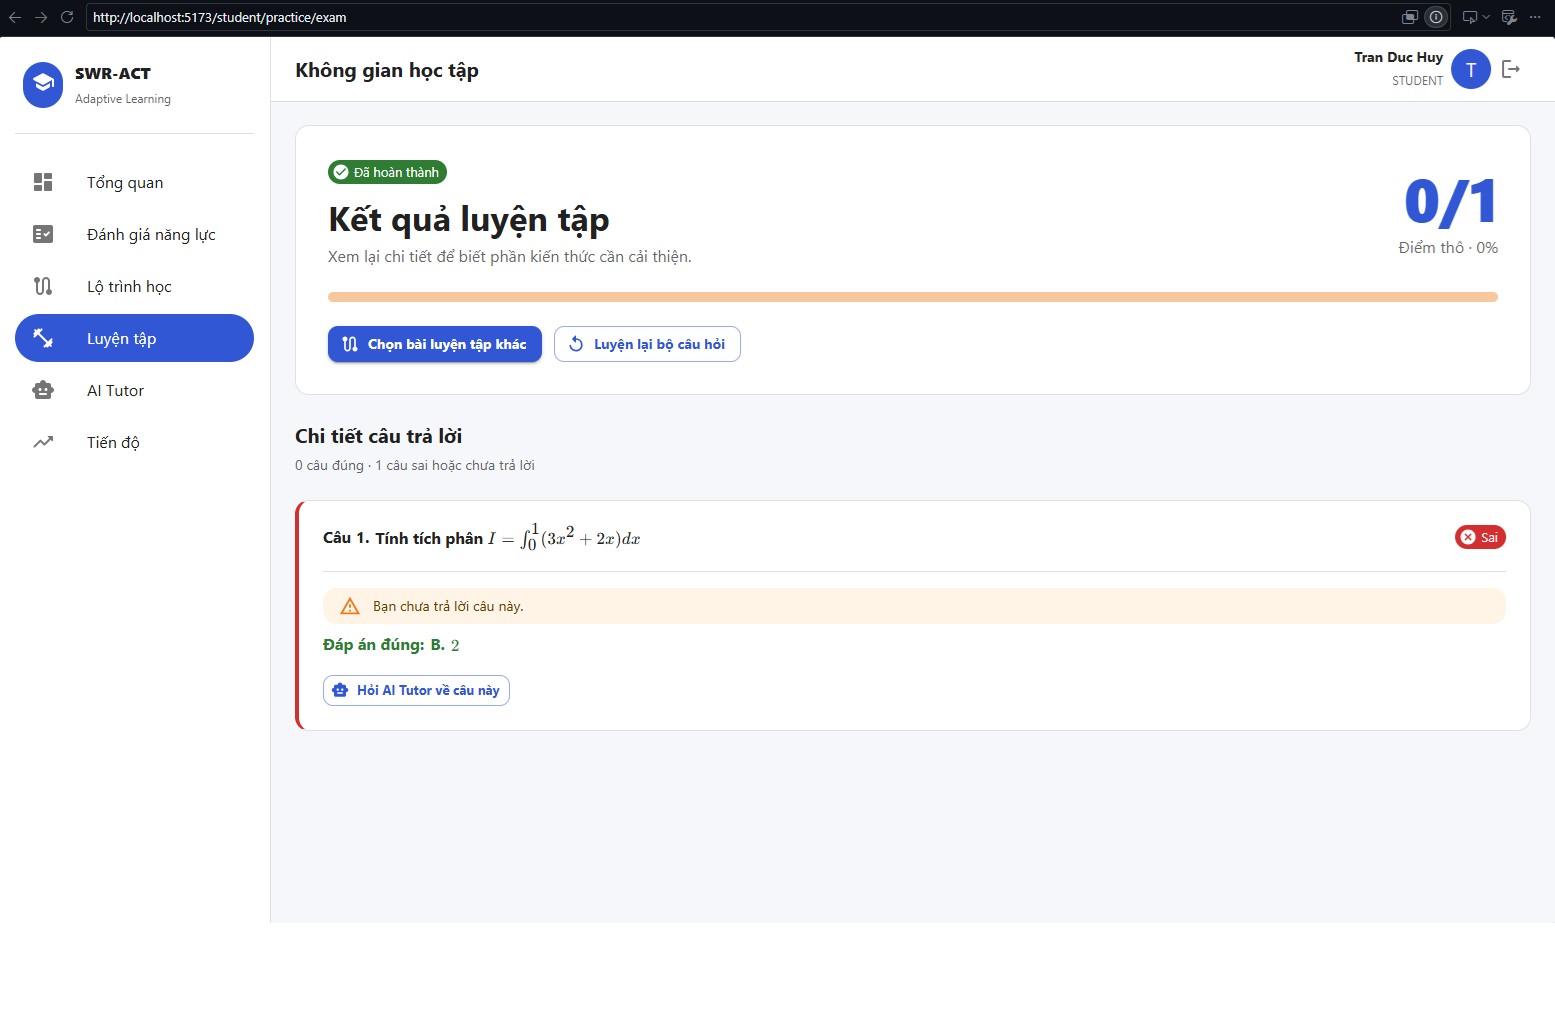
\includegraphics[width=1\textwidth]{figure_5_6_practice_result.png}
    \caption{Practice Result Breakdown with 'Ask AI Tutor' Integration Button}
    \label{fig:ui_practice_result}
\end{figure}

\subsubsection{Intelligent AI Tutor with RAG Integration (UC-04)}
\begin{itemize}[leftmargin=1.5em, itemsep=0.2em]
    \item \textbf{Functional Description:} Provides 24/7 Socratic pedagogical guidance. Instead of giving direct answers, the AI Tutor analyzes the student's selected wrong answer against the official explanation to guide their critical thinking process.
    \item \textbf{User Workflow \& UI Components:}
    \begin{enumerate}[leftmargin=1.5em, itemsep=0.1em]
        \item Clicking ``Hoi AI cau nay'' on an incorrect question seamlessly redirects the student to \texttt{/student/tutor} while automatically carrying the \texttt{question\_id} and problem metadata.
        \item The backend constructs a structured prompt combining the question statement, choices, correct key, official solution, and system pedagogical guardrails.
        \item The AI generates step-by-step hints and conceptual explanations formatted in Markdown and LaTeX.
    \end{enumerate}
    \item \textbf{Underlying APIs:} \texttt{POST /api/v1/rbac/tutor/ask}.
\end{itemize}

\begin{figure}[H]
    \centering
    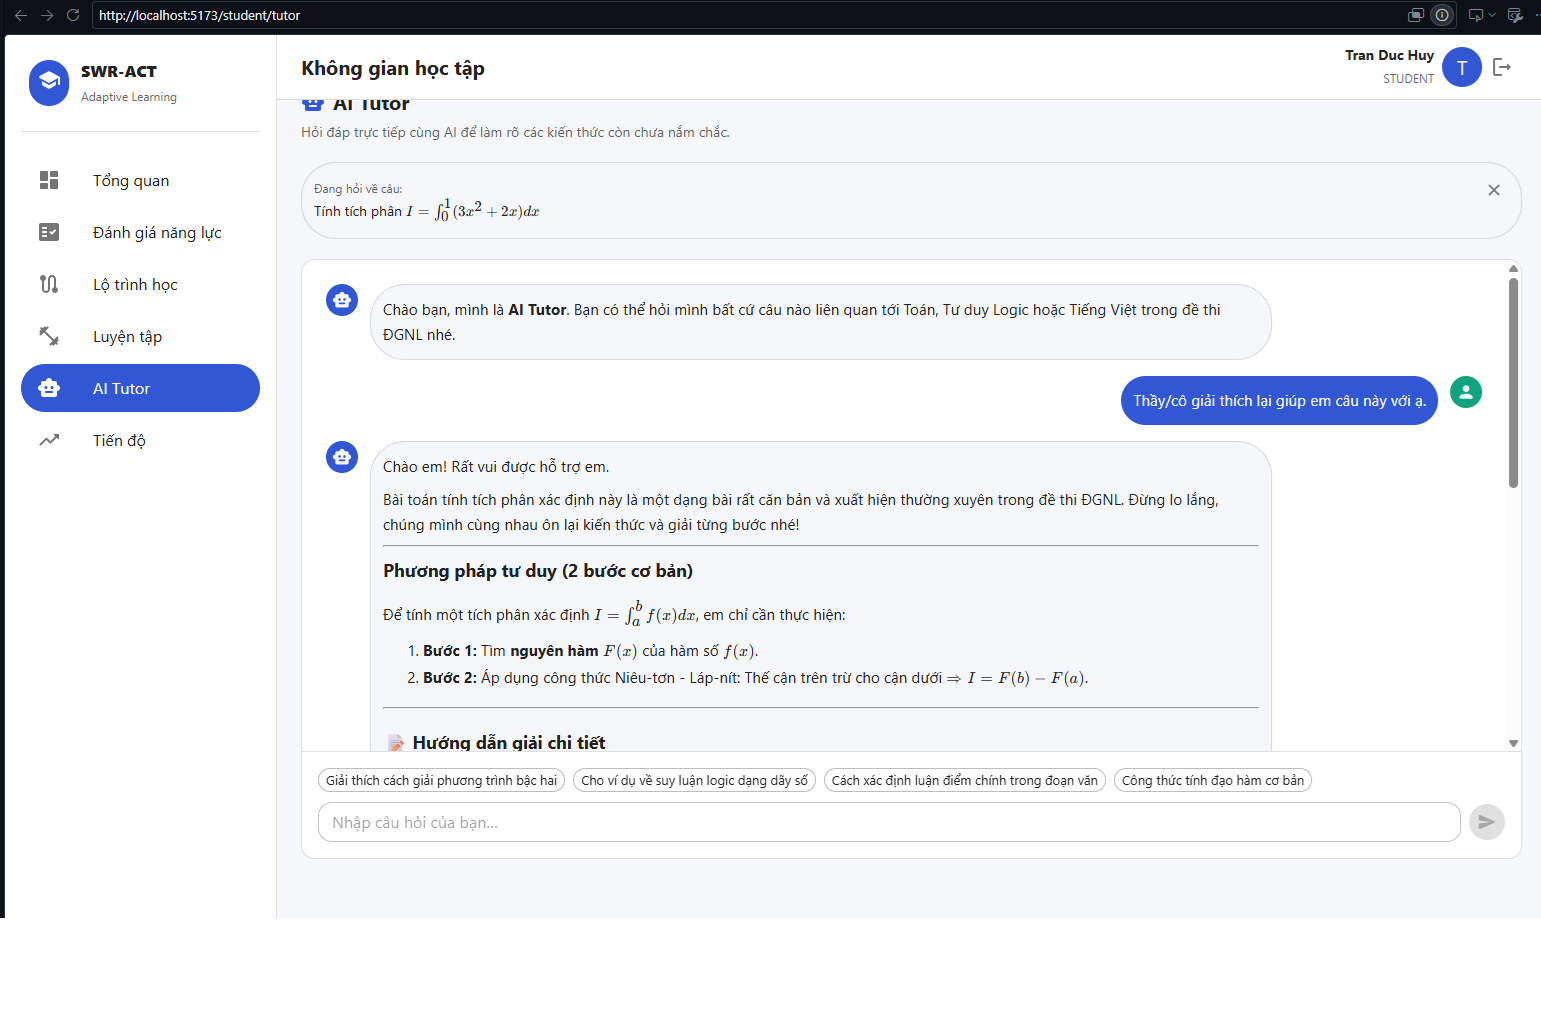
\includegraphics[width=0.82\textwidth]{figure_5_7_tutor.png}
    \caption{AI Tutor Pedagogical Explanation Interface with KaTeX Formulas}
    \label{fig:ui_tutor}
\end{figure}

\subsubsection{Student Overview \& Competency Progress Analytics Module (UC-05)}
\begin{itemize}[leftmargin=1.5em, itemsep=0.2em]
    \item \textbf{Functional Description:} Aggregates individual learning milestones and historical examination metrics into a unified progress dashboard. It delivers multidimensional competency profiling via radar charts and historical score progression curves to evaluate knowledge retention over time.
    \item \textbf{User Workflow \& UI Components:}
    \begin{itemize}[leftmargin=1.2em, itemsep=0.1em]
        \item \textit{Overview Dashboard (\texttt{/student}):} Displays real-time countdown widgets to the examination date, target score card ($S_{\text{target}}$), active daily study tasks retrieved via PlanTask, and recent practice test history logs.
        \item \textit{Competency Radar Chart (\texttt{/student/progress}):} Utilizes Recharts to render an interactive Polar Radar Chart mapping student accuracy across three core examination pillars: Mathematics, Logic Reasoning, and Vietnamese Language.
        \item \textit{Historical Score Trendline:} Renders a responsive Line Chart tracking daily test score percentages, paired with an algorithmic score prediction card ($S_{\text{predict}} \in [1, 1200]$) derived from the mean and observed standard deviation of completed tests.
    \end{itemize}
    \item \textbf{Underlying APIs:} \texttt{GET /api/study-plan/current}, \texttt{GET /api/practice/history}, \texttt{GET /api/analytics/progress}.
\end{itemize}

\begin{figure}[H]
    \centering
    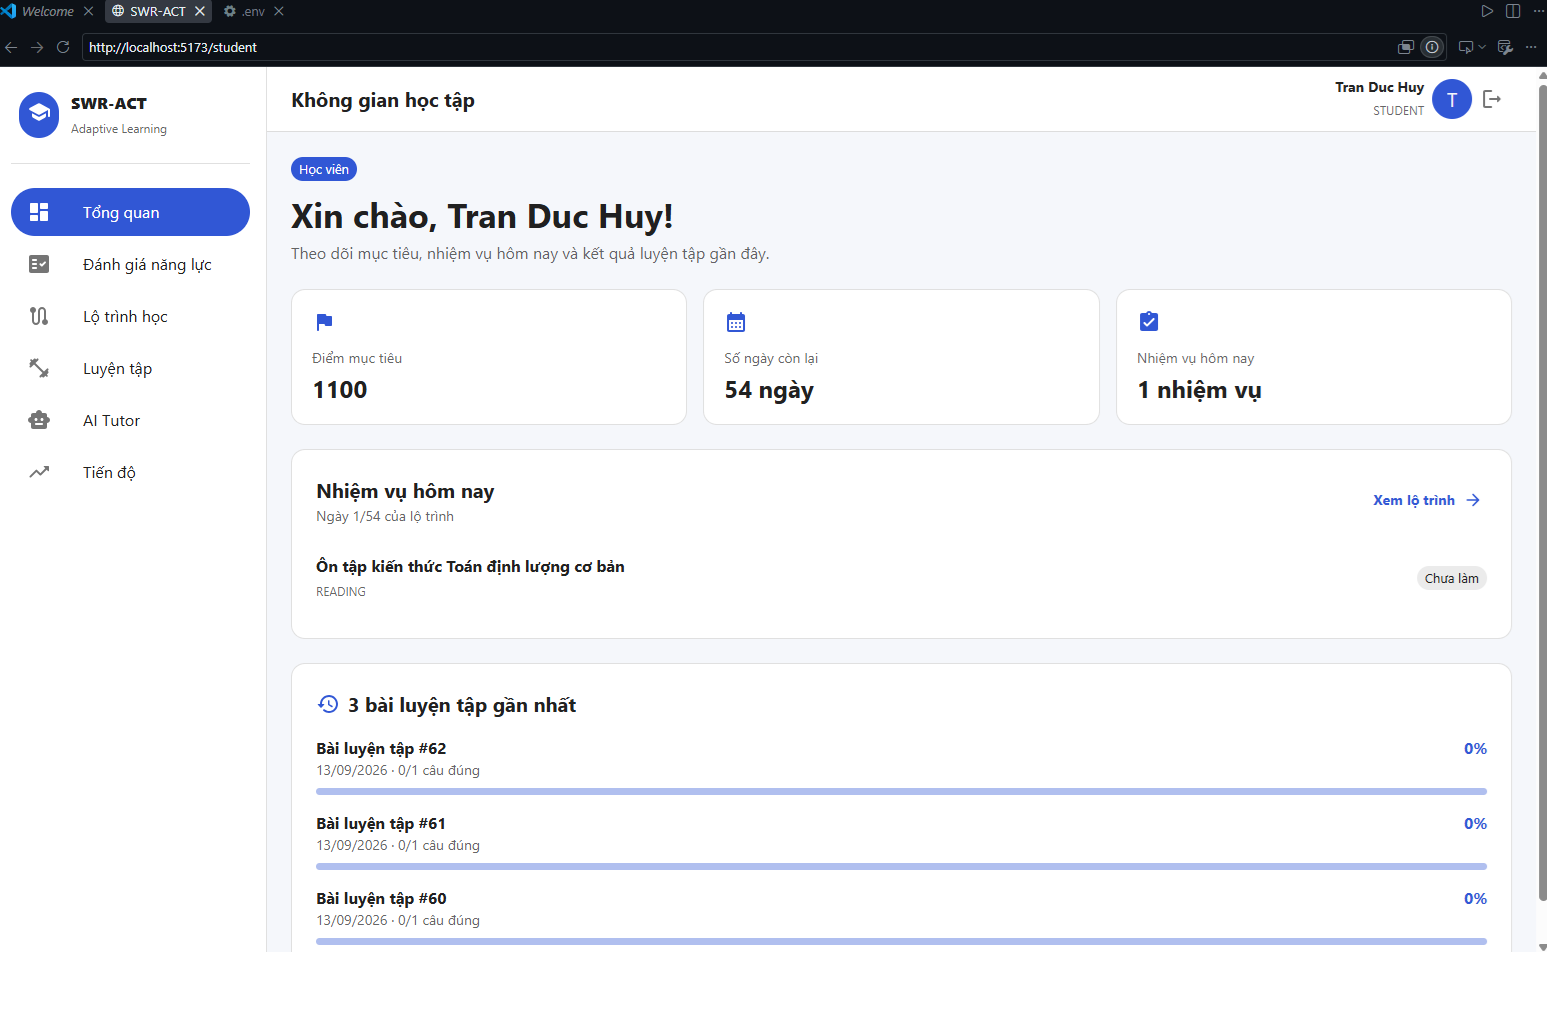
\includegraphics[width=1\textwidth]{figure_5_8_student_overview.png}
    \caption{Student Overview Dashboard and Daily Learning Tasks Tracking}
    \label{fig:ui_student_overview}
\end{figure}

\begin{figure}[H]
    \centering
    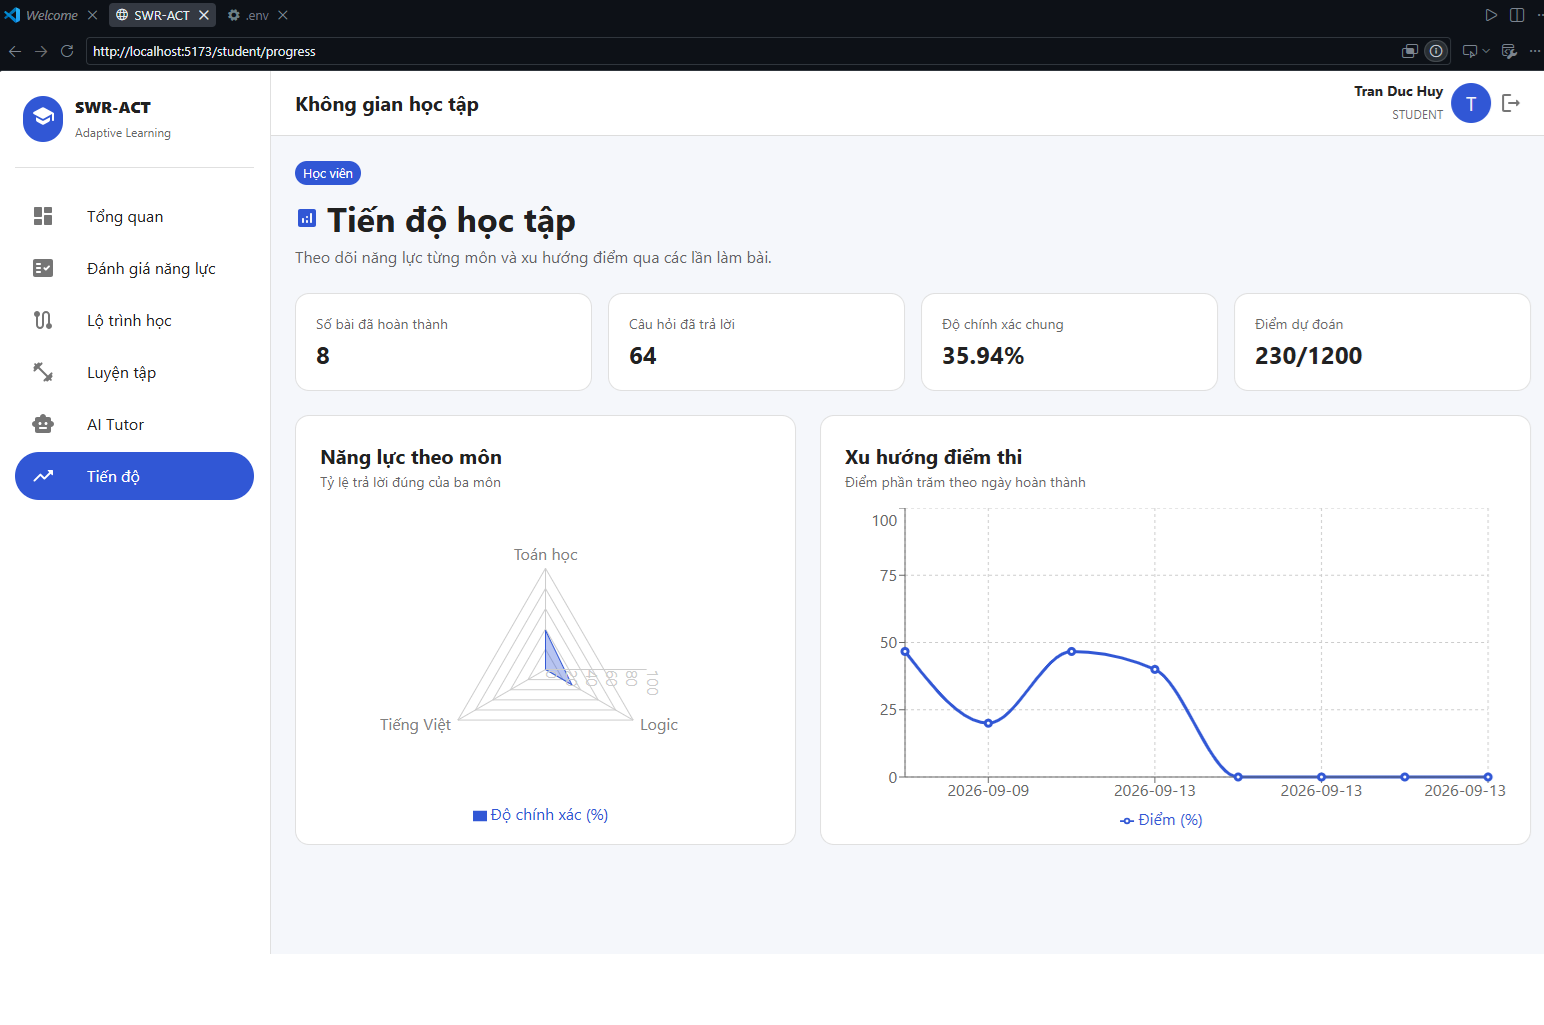
\includegraphics[width=1\textwidth]{figure_5_9_student_progress.png}
    \caption{Student Competency Analytics with Radar Accuracy and Historical Score Curves}
    \label{fig:ui_student_progress}
\end{figure}

\subsubsection{Teacher Portal: Question Bank Management System (CRUD) (UC-06)}
\begin{itemize}[leftmargin=1.5em, itemsep=0.2em]
    \item \textbf{Functional Description:} Grants pedagogical staff full administrative governance over the central question repository, enforcing multi-criteria search, pagination, and real-time mathematical validation before persistence.
    \item \textbf{User Workflow \& UI Components:}
    \begin{itemize}[leftmargin=1.2em, itemsep=0.1em]
        \item \textit{Central Data Table (\texttt{/teacher/questions}):} Renders a responsive question bank table protected by TEACHER and ADMIN RBAC guards. Supports dynamic keyword search on question stems, subject filters, topic selectors, and difficulty chips (EASY, MEDIUM, HARD).
        \item \textit{Interactive Question Modal Form:} Empowers instructors to execute Create, Read, Update, and Delete (CRUD) operations. The form provides decoupled inputs for four choices (A, B, C, D), correct key designation, and detailed pedagogical rationale.
        \item \textit{Real-Time KaTeX Math Preview:} Features an integrated live preview toggle powered by MathMarkdown, ensuring complex mathematical equations, matrices, and LaTeX notation render without formatting errors prior to database submission.
    \end{itemize}
    \item \textbf{Underlying APIs:} \texttt{GET /api/teacher/questions}, \texttt{POST /api/teacher/questions}, \texttt{PUT /api/teacher/questions/\{id\}}, \texttt{DELETE /api/teacher/questions/\{id\}}.
\end{itemize}

\begin{figure}[H]
    \centering
    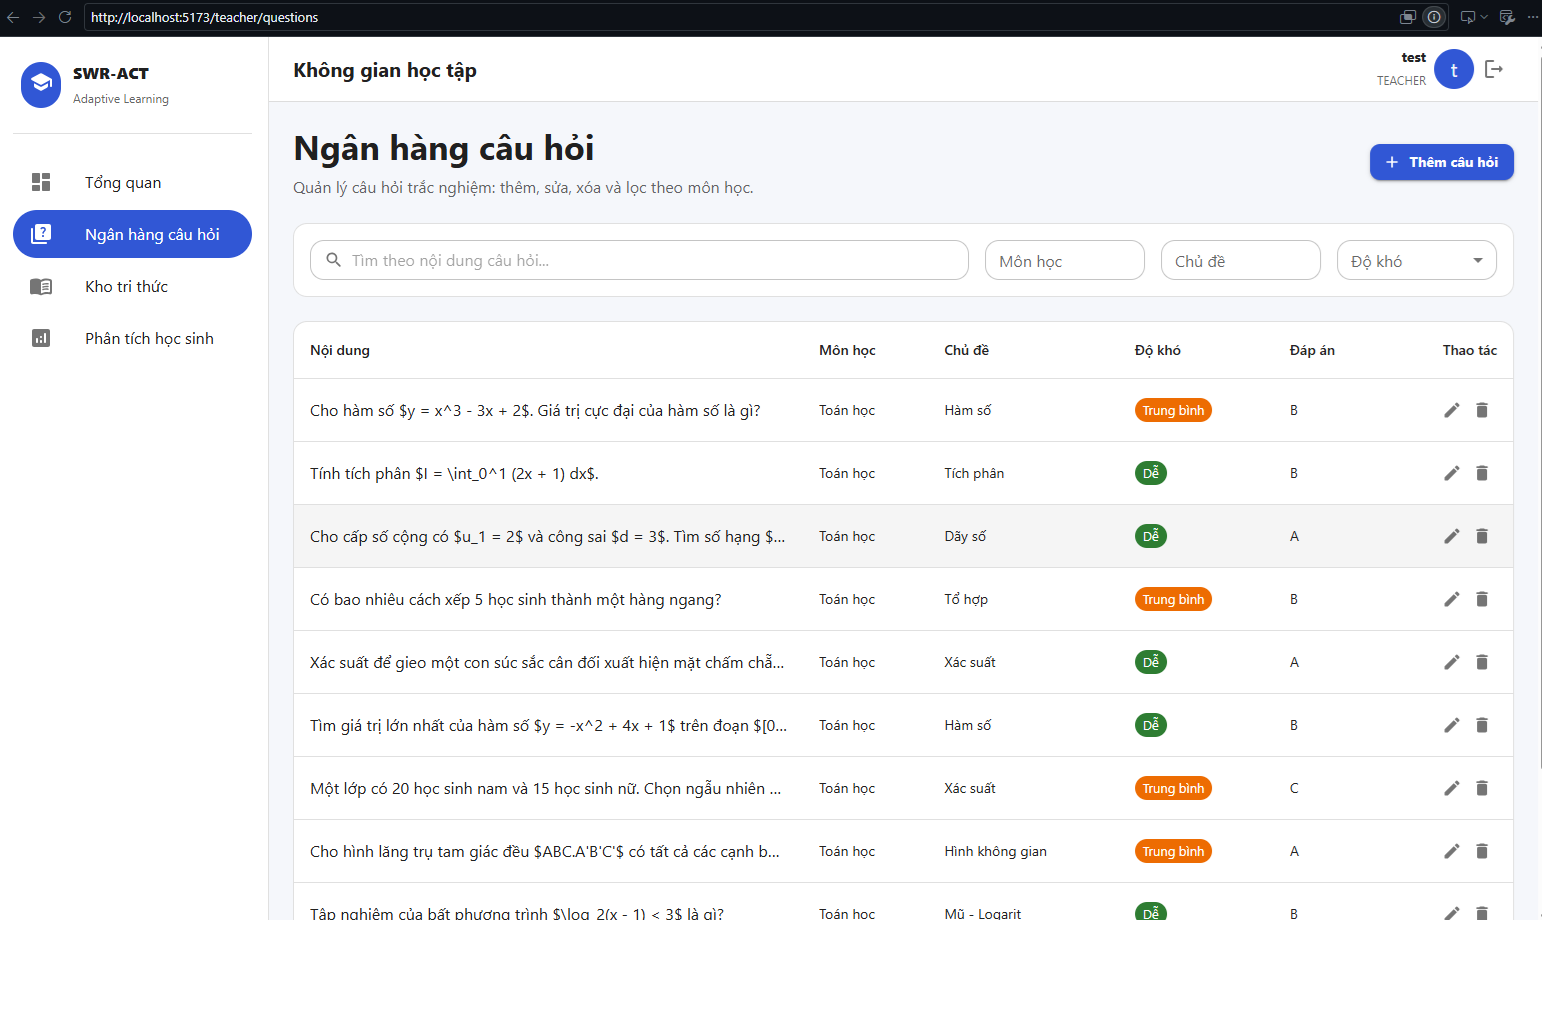
\includegraphics[width=0.82\textwidth]{figure_5_10_question_bank.png}
    \caption{Teacher Question Bank Data Table with Filter and Pagination Controls}
    \label{fig:ui_question_bank}
\end{figure}

\begin{figure}[H]
    \centering
    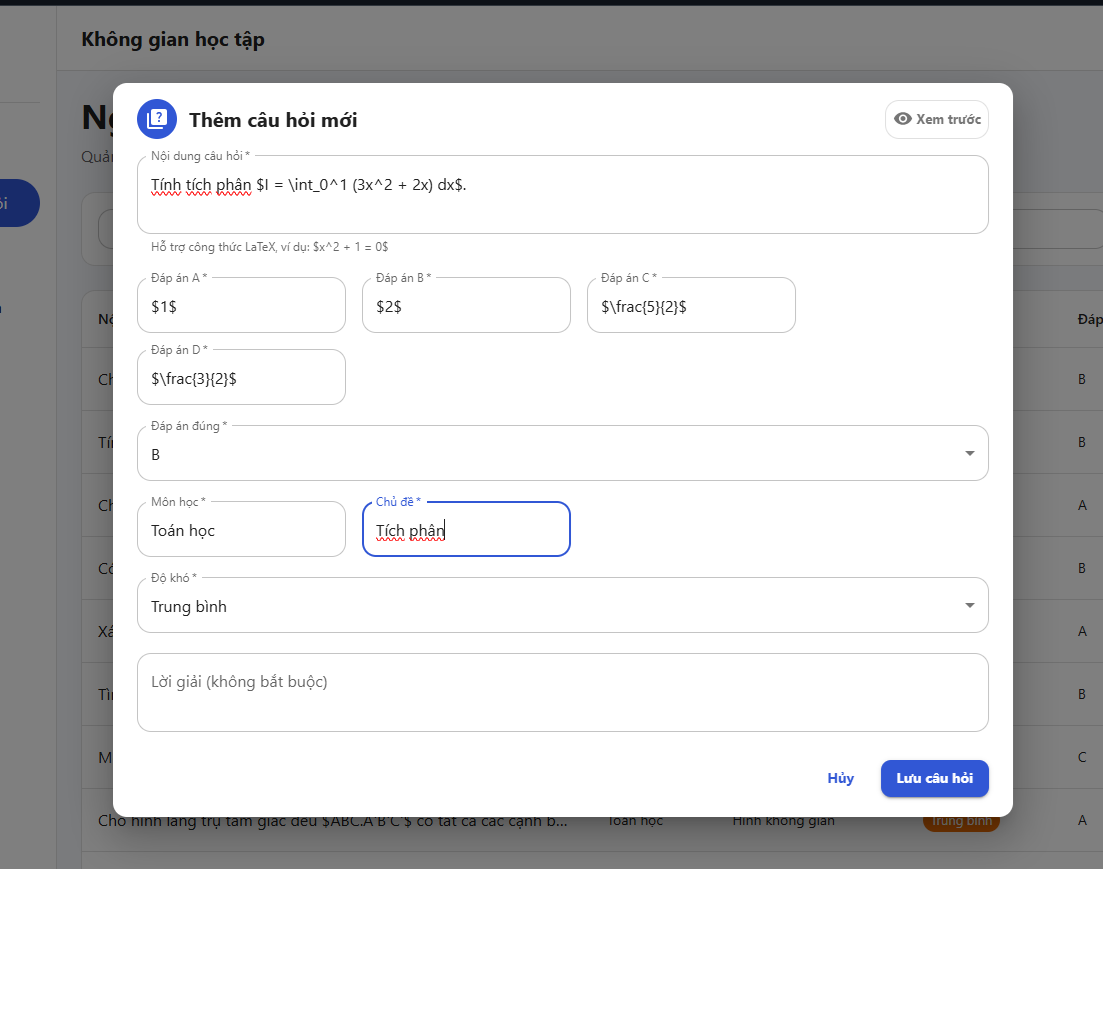
\includegraphics[width=1\textwidth]{figure_5_11_question_modal.png}
    \caption{Question Modal Interface featuring Real-Time KaTeX Math Rendering Preview}
    \label{fig:ui_question_modal}
    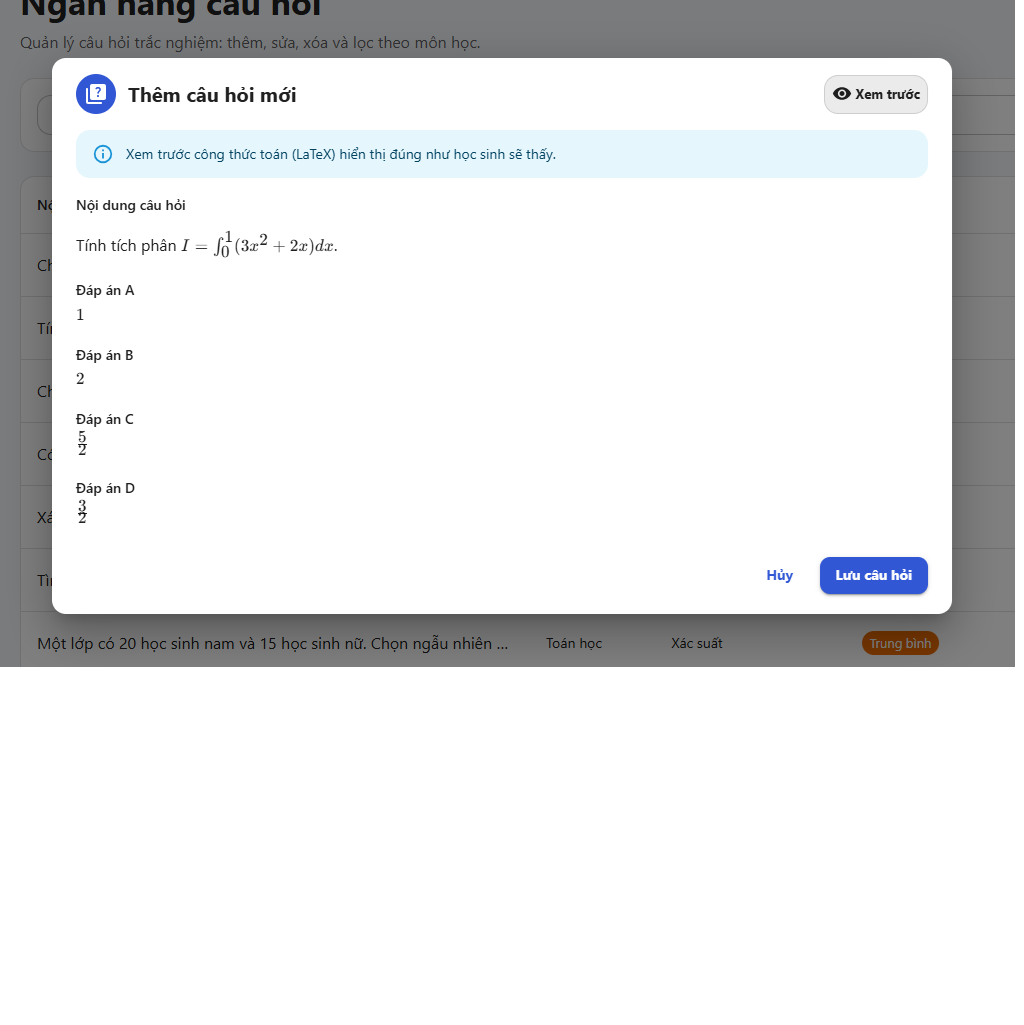
\includegraphics[width=1\textwidth]{figure_5_11_question_modal_2.png}
\end{figure}

\subsubsection{Teacher Portal: Class-Wide Performance Analytics (UC-07)}
\begin{itemize}[leftmargin=1.5em, itemsep=0.2em]
    \item \textbf{Functional Description:} Provides high-level cohort telemetry for instructors, summarizing student engagement, test completion volumes, and subject-level academic proficiencies across the entire student population.
    \item \textbf{User Workflow \& UI Components:}
    \begin{itemize}[leftmargin=1.2em, itemsep=0.1em]
        \item \textit{Cohort Metric Cards (\texttt{/teacher/analytics}):} Summarizes primary system KPIs including Total Enrolled Students (\texttt{role = STUDENT}) and Total Completed Submissions (\texttt{status = COMPLETED}).
        \item \textit{Subject-Level Proficiency Distribution:} Visualizes normalized mean scores across knowledge domains, highlighting general performance baselines to assist teachers in adjusting classroom curriculum.
    \end{itemize}
    \item \textbf{Underlying APIs:} \texttt{GET /api/teacher/analytics/overview}.
\end{itemize}

\begin{figure}[H]
    \centering
    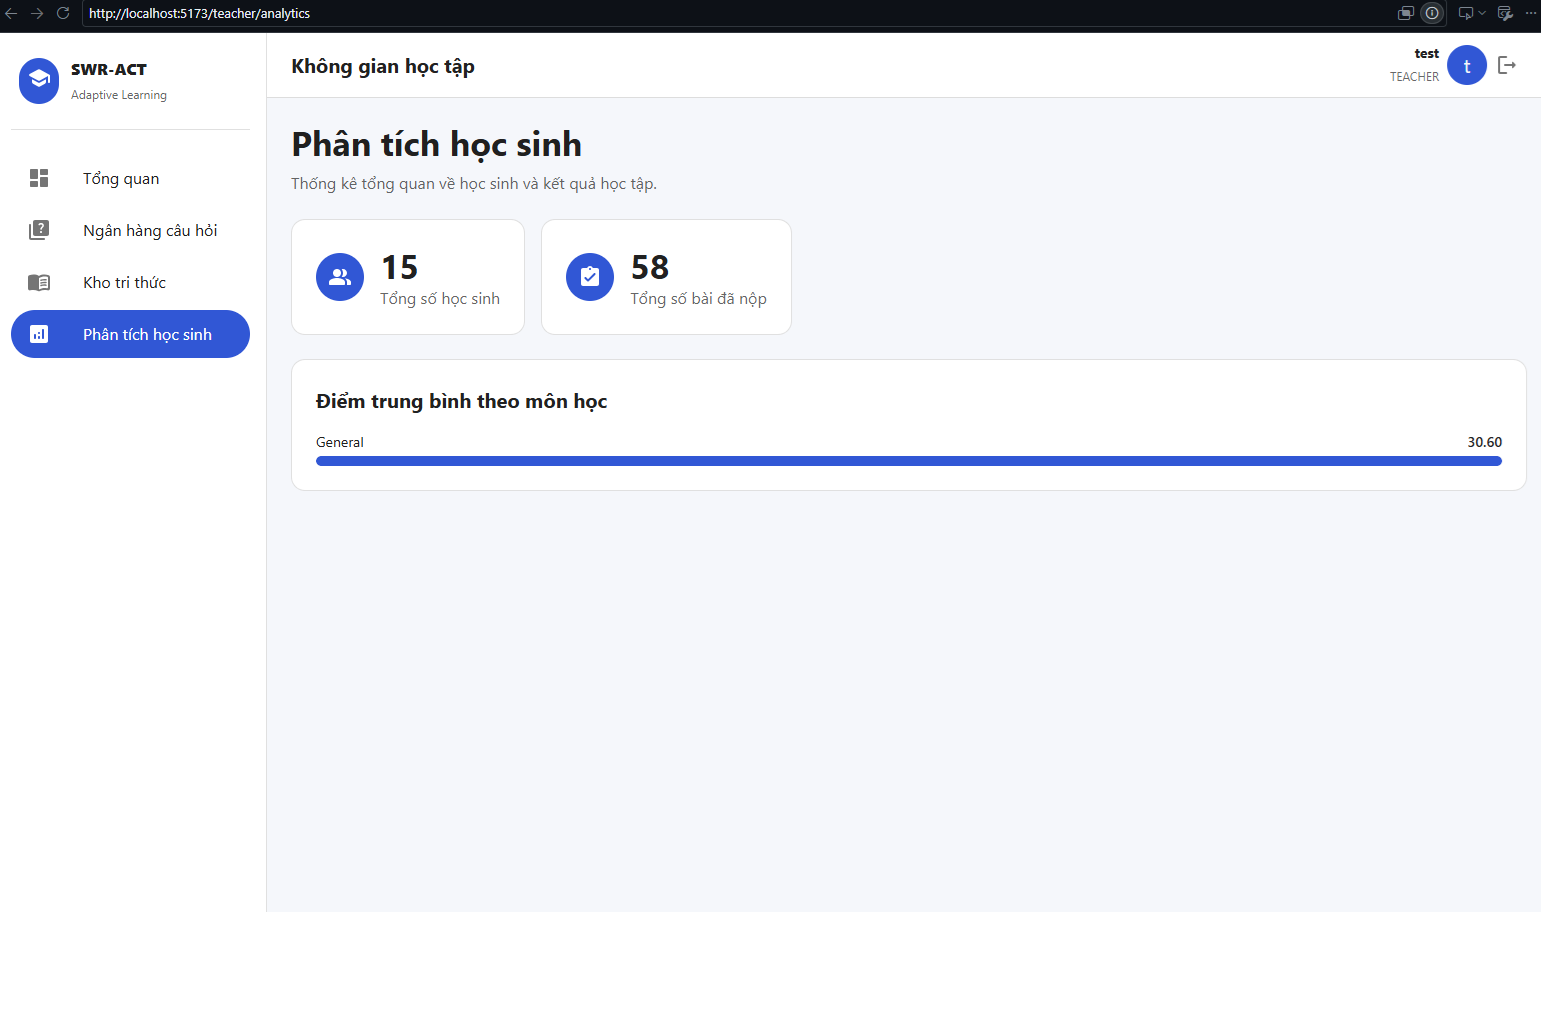
\includegraphics[width=1\textwidth]{figure_5_12_teacher_analytics.png}
    \caption{Teacher Class Performance Overview and Subject Score Distribution}
    \label{fig:ui_teacher_analytics}
\end{figure}

\subsubsection{Parent Portal Subsystem}
\begin{itemize}[leftmargin=1.5em, itemsep=0.2em]
    \item \textbf{Functional Description \& System Architecture:} The Parent Portal module is designed to provide guardians with direct, transparent visibility into their children's academic trajectory and competency preparation for the National High School Graduation and Competency Assessment exams (DGNL). Secured under strict Role-Based Access Control (\texttt{UserRole.PARENT}), this subsystem queries relational mappings in the \texttt{student\_parents} table and performs analytical aggregations against \texttt{study\_plans}, \texttt{tests}, and \texttt{user\_answers}.
    \item \textbf{Key Features Include:}
    \begin{itemize}[leftmargin=1.2em, itemsep=0.1em]
        \item \textit{Academic Goal Tracking \& Countdown:} Dynamically extracts the active study plan target score ($S_{\text{target}} \in [1, 1200]$) and calculates remaining preparation days until target completion.
        \item \textit{Multi-Subject Competency Radar:} Renders a balanced radar chart illustrating student proficiency across core domains: Mathematics, Logical Thinking, and Vietnamese Language.
        \item \textit{Performance Trajectory \& Prediction:} Visualizes chronological exam scores accompanied by dynamic upper/lower bound confidence intervals for real exam performance forecasting.
    \end{itemize}
\end{itemize}

\begin{figure}[H]
    \centering
    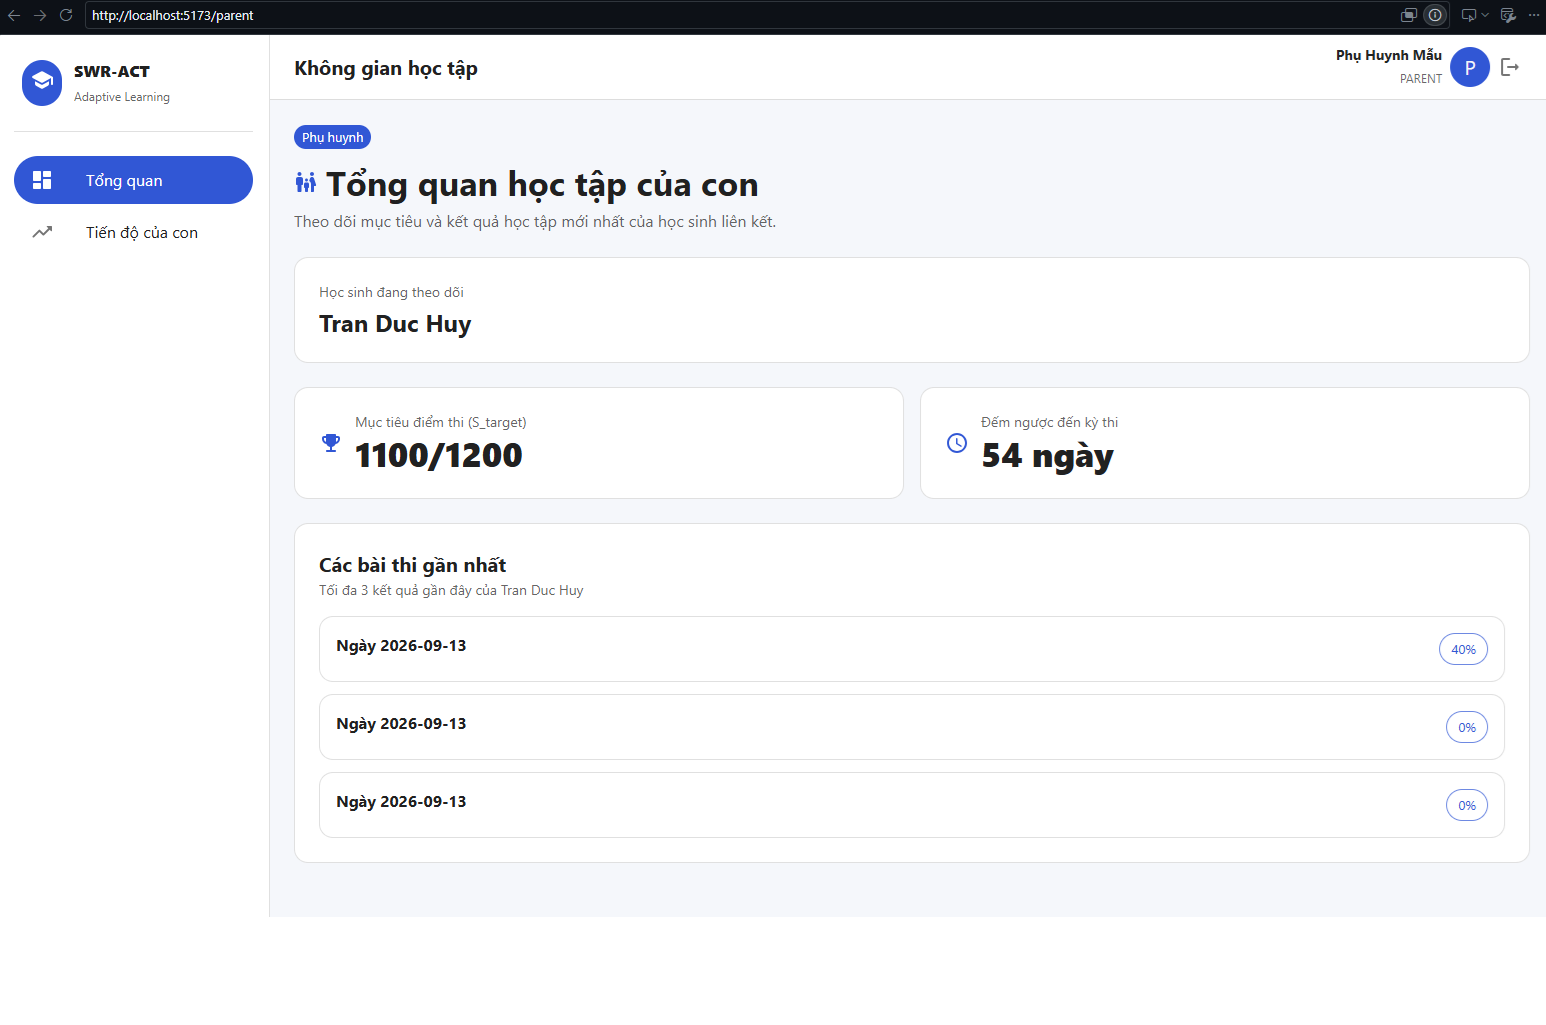
\includegraphics[width=1\textwidth]{figure_5_13_parent_overview.png}
    \caption{Parent Portal Overview Dashboard}
    \label{fig:ui_parent_overview}
\end{figure}

\begin{figure}[H]
    \centering
    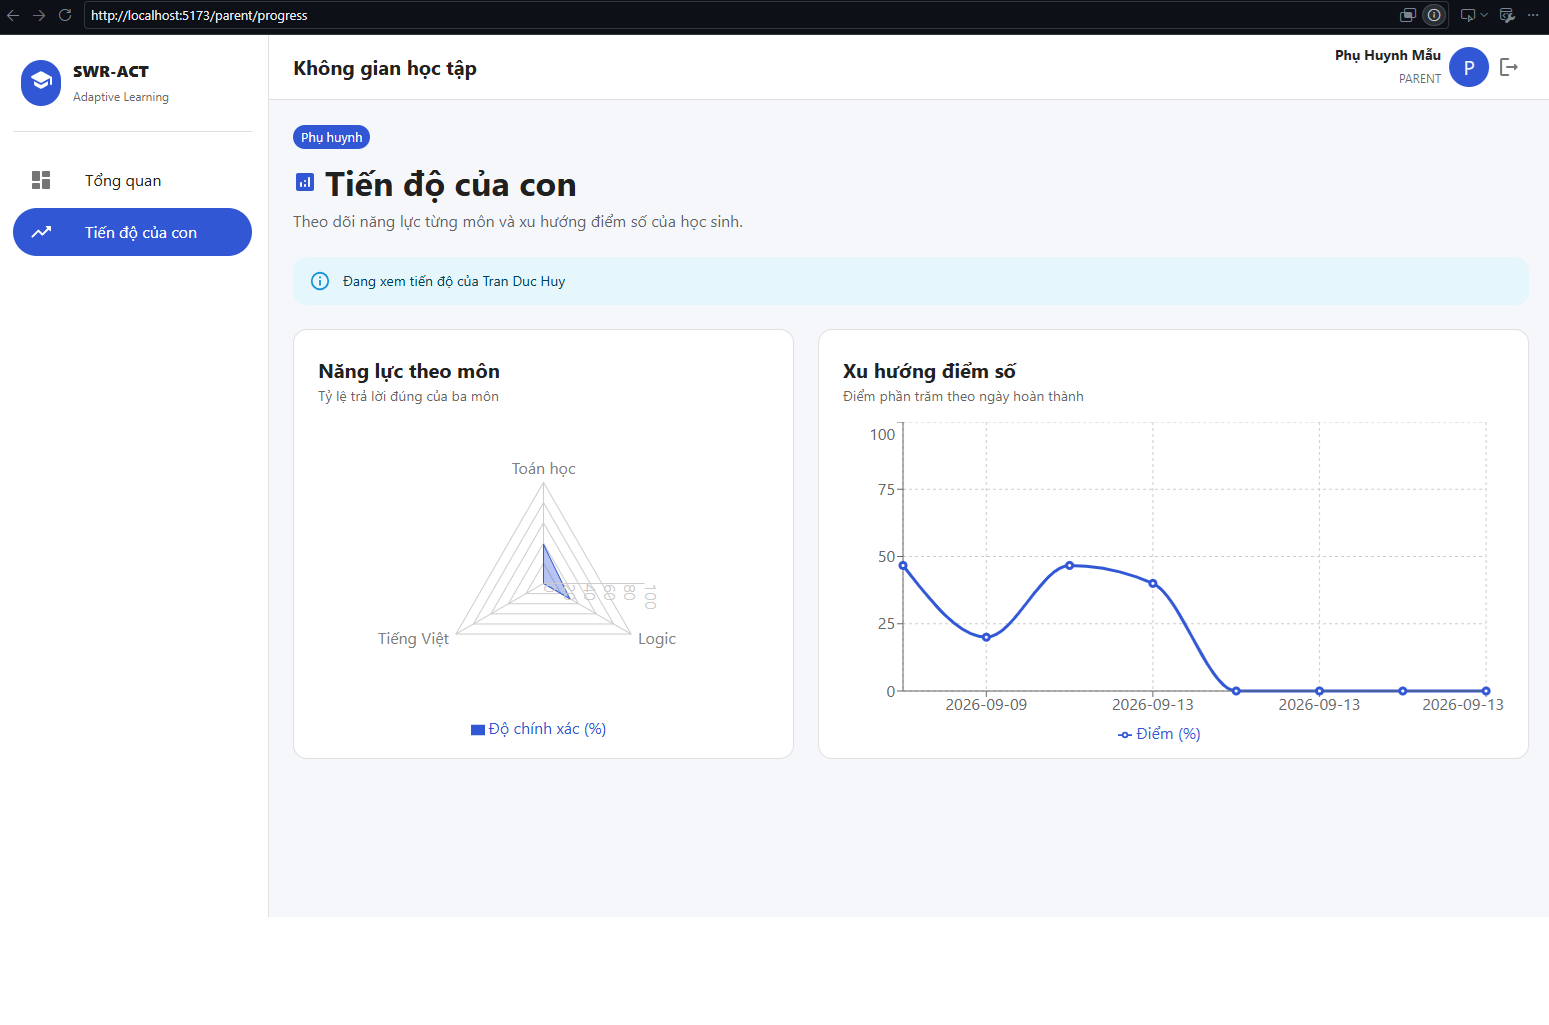
\includegraphics[width=1\textwidth]{figure_5_14_parent_progress.png}
    \caption{Parent Portal Progress Tracking with Multi-Subject Visualizations}
    \label{fig:ui_parent_progress}
\end{figure}

\subsubsection{Teacher Overview \& Knowledge Base (RAG)}
\begin{itemize}[leftmargin=1.5em, itemsep=0.2em]
    \item \textbf{Functional Description \& RAG Retrieval Pipeline:} The Teacher Management Subsystem equips instructional staff with macroscopic telemetry and semantic knowledge retrieval verification tools. Protected under \texttt{require\_roles(UserRole.TEACHER, UserRole.ADMIN)}, this module couples aggregate administrative data with the core Retrieval-Augmented Generation (RAG) semantic pipeline.
    \item \textbf{Key Features Include:}
    \begin{itemize}[leftmargin=1.2em, itemsep=0.1em]
        \item \textit{Systemic Metrics Telemetry:} Delivers dynamic counter statistics on total question bank inventory, active student enrollment, and cumulative test submissions categorized by subject area.
        \item \textit{Semantic Knowledge Base (RAG Verification):} Connects to the \texttt{/api/v1/rag/query} pipeline. Educators provide reference pedagogical texts and query prompts; the backend executes sliding-window chunking, generates normalized embeddings, and returns top-ranked relevant passages scored by Cosine Similarity ($S_c \in [-1.0, 1.0]$).
        \item \textit{Interoperability \& Shared Engine:} Maintains backward-compatible authorization policies ensuring both educators (\texttt{TEACHER}) and learners (\texttt{STUDENT}) leverage the identical inference engine without RBAC collisions.
    \end{itemize}
\end{itemize}

\begin{figure}[H]
    \centering
    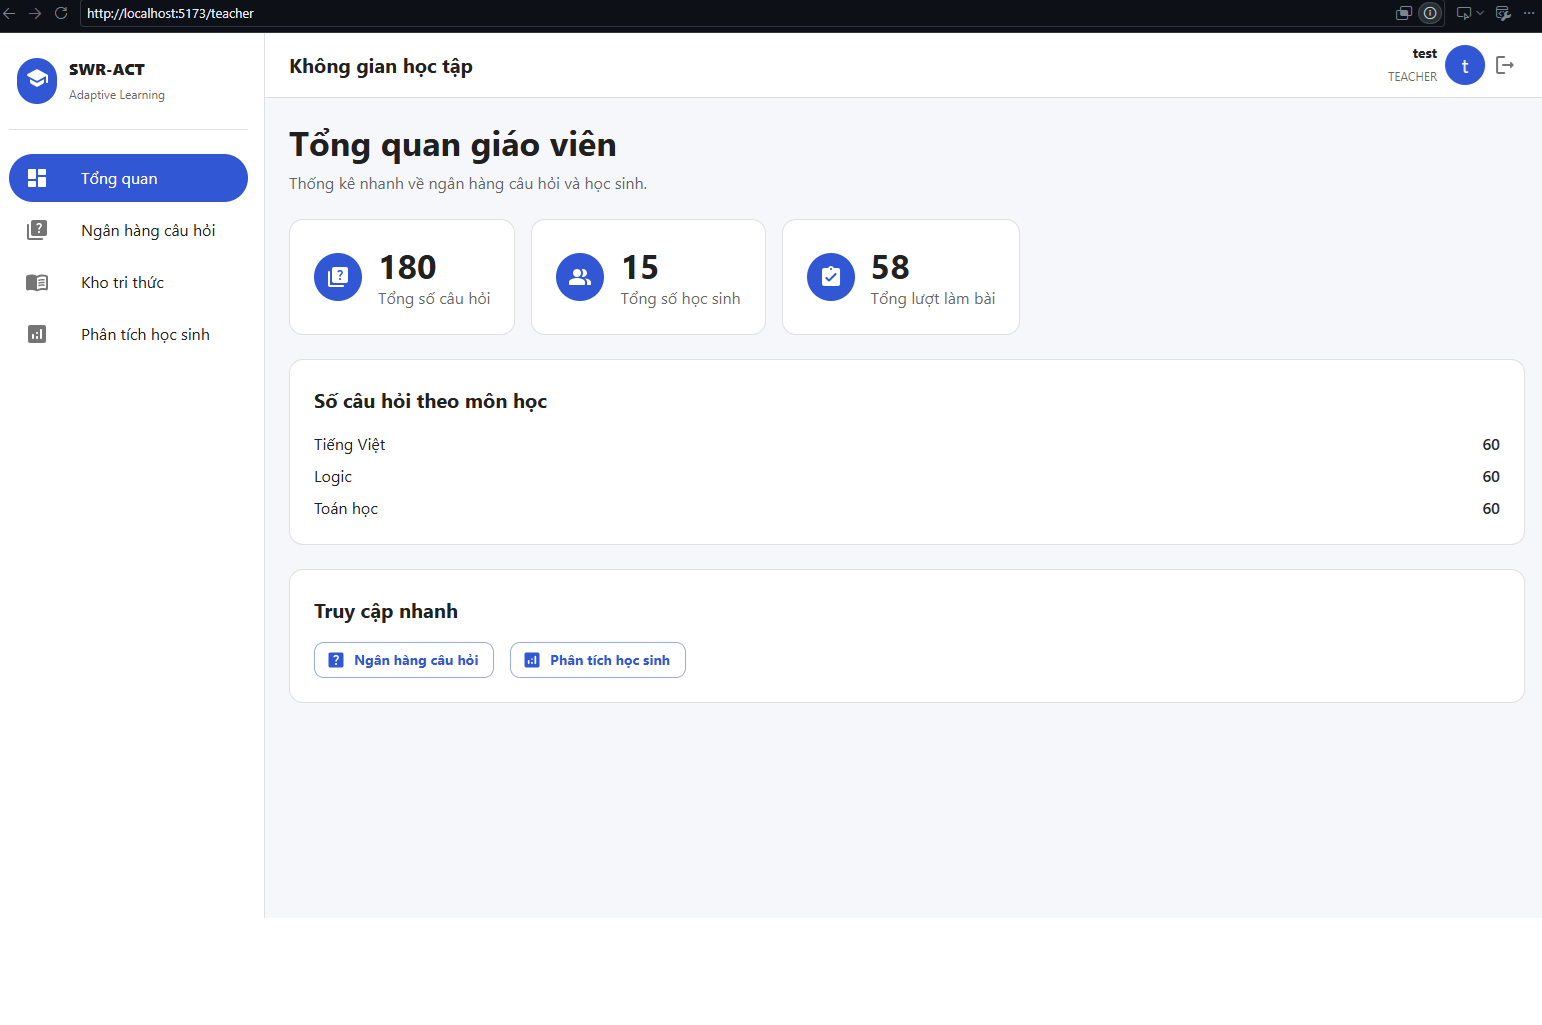
\includegraphics[width=1\textwidth]{figure_5_15_teacher_overview.png}
    \caption{Teacher Overview Analytics Dashboard}
    \label{fig:ui_teacher_overview}
\end{figure}

\begin{figure}[H]
    \centering
    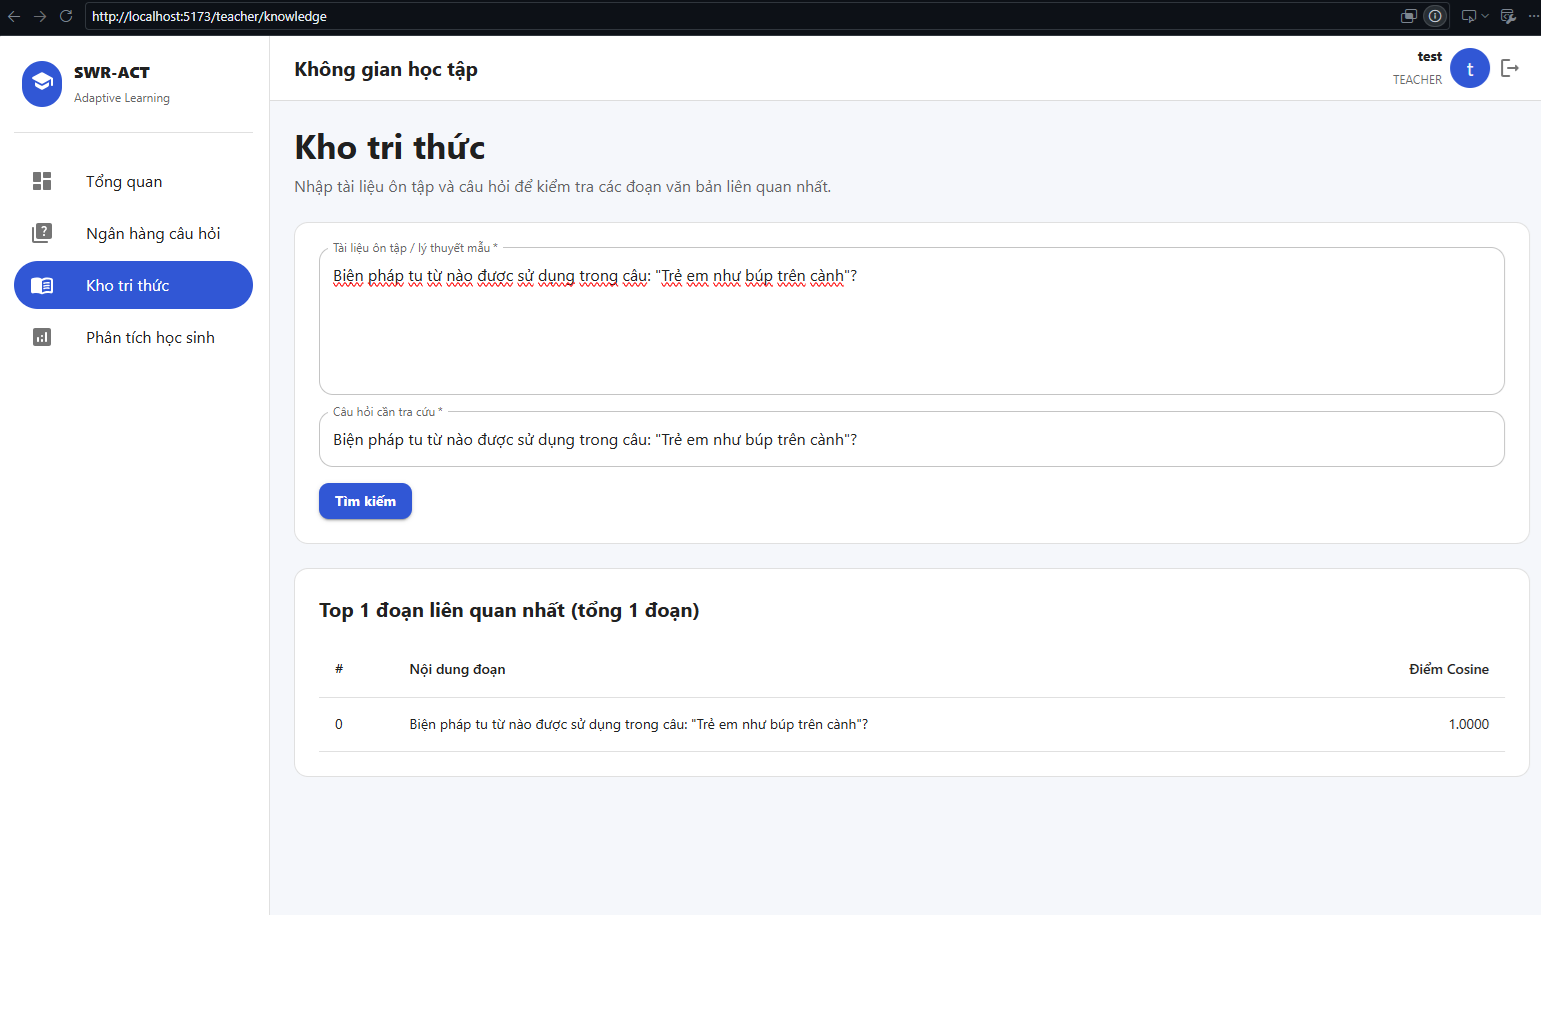
\includegraphics[width=1\textwidth]{figure_5_16_teacher_rag.png}
    \caption{Teacher Knowledge Base Semantic Retrieval Verification Interface}
    \label{fig:ui_teacher_rag}
\end{figure}

\subsection{Automated Unit \& Integration Testing Results}
To verify overall system stability, regression resilience, and ensure strict compliance across all core modules (Authentication, 4-Role RBAC, RAG Pipeline, Adaptive Practice, Diagnostic Assessment, Learning Roadmaps, Analytics Engine, Teacher Management, and Parent Portal Monitoring), an automated test suite was constructed and executed via Pytest.

\begin{itemize}[leftmargin=1.5em, itemsep=0.2em]
    \item \textbf{Test Execution Result:} 56/56 Tests Passed (100\% Pass Rate).
    \item \textbf{Total Execution Time:} $\sim$8.06s seconds.
    \item \textbf{Test Environment:} Isolated SQLite Database engine with transactional session rollback fixtures and Asynchronous Mocking Stubs (\texttt{unittest.mock.AsyncMock}).
\end{itemize}

\begin{figure}[H]
    \centering
    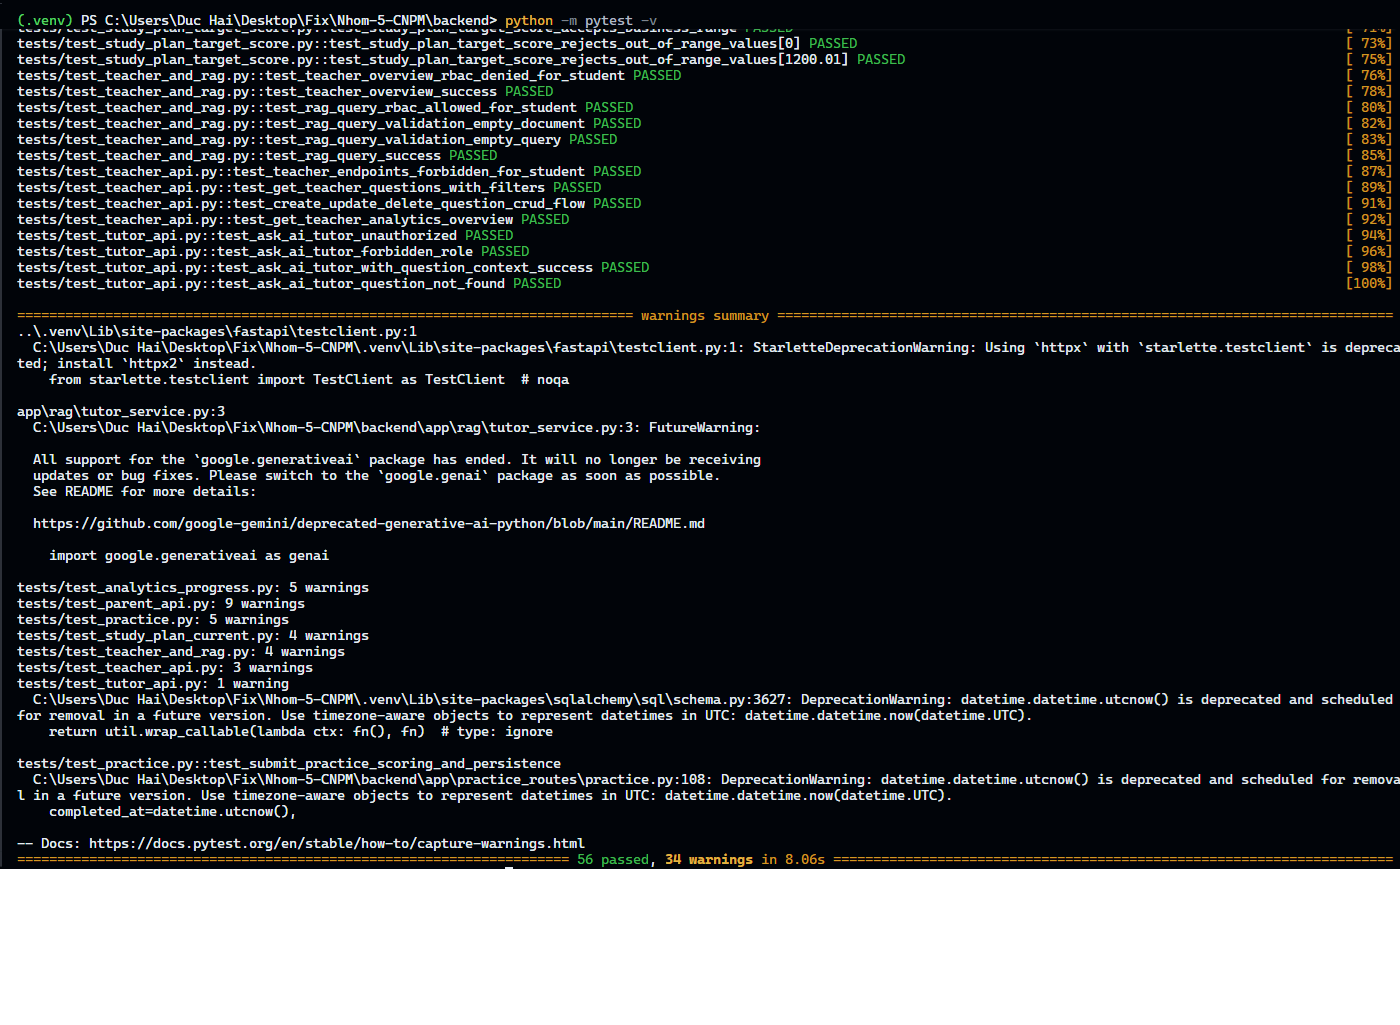
\includegraphics[width=1\textwidth]{figure_pytest_terminal.png}
    \caption{Automated Pytest Execution Results across 13 Test Suites (56/56 Passed)}
    \label{fig:pytest_terminal}
\end{figure}

\subsubsection*{Verified Modules \& Test Suites Summary}
\begin{enumerate}[leftmargin=1.5em, itemsep=0.2em]
    \item \textbf{Integration \& Auth Suite} (\texttt{tests/test\_integration.py} - Passed 8/8 tests): Validates user schema mapping, student registration, duplicate email handling (HTTP 409 Conflict), login token generation, user profile inspection (\texttt{/me}), refresh token rotation, inactive user access locking, and full 4-role RBAC authorization matrix enforcement.
    \item \textbf{JWT Contract Suite} (\texttt{tests/test\_jwt\_contract.py} - Passed 4/4 tests): Verifies access token claims (\texttt{sub}, \texttt{role}, \texttt{type}, \texttt{jti}, \texttt{exp}), refresh token lifespan integrity, rejection of expired cryptographic signatures, and Bcrypt password verification.
    \item \textbf{RAG Pipeline Suite} (\texttt{tests/test\_rag.py} - Passed 3/3 tests): Tests text chunking sliding window algorithm (chunk size = 100, overlap = 20), L2 vector normalization (magnitude = 1.0), and Cosine Similarity Top-K semantic retrieval.
    \item \textbf{Standalone RBAC Suite} (\texttt{tests/test\_rbac\_standalone.py} - Passed 7/7 tests): Validates isolated dependency injection permission guards and verifies HTTP 403 Forbidden enforcement on unauthorized role requests.
    \item \textbf{SDD Compliance Suite} (\texttt{tests/test\_sdd.py} - Passed 1/1 test): Validates architectural documentation and API contract consistency against the Software Design Document.
    \item \textbf{Study Plan \& Goal Suite} (\texttt{tests/test\_study\_plan\_target\_score.py} - Passed 4/4 tests): Verifies database \texttt{NUMERIC(7,2)} precision for target scores up to 1200 points and enforces business validation constraints on out-of-range inputs.
    \item \textbf{Practice Module Suite} (\texttt{tests/test\_practice.py} - Passed 5/5 tests): Tests practice question querying with subject/topic/difficulty filters, STUDENT role enforcement, automated score calculation, test persistence, and completed practice history retrieval.
    \item \textbf{AI Tutor API Suite} (\texttt{tests/test\_tutor\_api.py} - Passed 4/4 tests): Verifies HTTP 401 on unauthenticated access, HTTP 403 on invalid roles (PARENT), HTTP 404 on missing questions, and successful context-aware AI tutor response generation with mocked Gemini API calls.
    \item \textbf{Active Study Plan Suite} (\texttt{tests/test\_study\_plan\_current.py} - Passed 3/3 tests): Validates retrieval of the student's currently active study roadmap (\texttt{/api/study-plan/current}), returns structured daily tasks (\texttt{PlanTask}), and enforces HTTP 404 handling when no active roadmap exists.
    \item \textbf{Student Analytics \& Progress Suite} (\texttt{tests/test\_analytics\_progress.py} - Passed 3/3 tests): Verifies competency accuracy calculations broken down by academic subjects (Toán học, Logic, Tiếng Việt), historical daily score tracking, and predicted exam score range generation ($S_{\text{predict}} \in [1, 1200]$).
    \item \textbf{Teacher Management API Suite} (\texttt{tests/test\_teacher\_api.py} - Passed 4/4 tests): Validates teacher-exclusive RBAC permissions (rejecting student access with HTTP 403), full CRUD question bank operations (Create, Read with pagination/filters, Update, Delete), and system-wide student performance analytics overview.
    \item \textbf{Teacher Overview \& RAG Retrieval Suite} (\texttt{tests/test\_teacher\_and\_rag.py} - Passed 6/6 tests): Validates the \texttt{GET /api/teacher/overview} endpoint for aggregate question counts, student counts, and attempt analytics; enforces RBAC restriction (HTTP 403 for students on teacher overview); validates the semantic RAG pipeline (\texttt{/api/v1/rag/query}) for both TEACHER and STUDENT roles (HTTP 200 OK); and verifies input validations on empty query/document payloads.
    \item \textbf{Parent Portal API Suite} (\texttt{tests/test\_parent\_api.py} - Passed 4/4 tests): Validates unauthenticated request rejection (HTTP 401 Unauthorized); verifies RBAC enforcement against student access (HTTP 403 Forbidden); handles edge cases for parent accounts without linked children; and verifies successful data aggregation on \texttt{GET /api/parent/overview} and \texttt{GET /api/parent/progress} including subject accuracy radar metrics, daily exam scores, and score predictions.
\end{enumerate}

\end{document}